\documentclass[
	12pt,
	a4paper,
	abstract,
	bibliography=totoc,
	chapterprefix,
	headings=openright,
	numbers=endperiod,
	parskip=half,
	twoside,
]{scrreprt}

\usepackage[T1]{fontenc}
\usepackage[utf8]{inputenc}

\usepackage{libertinus}
\usepackage[varqu,scaled=0.95]{inconsolata}
\usepackage{newtxmath}

\usepackage[english]{babel}

% Use less space for the page number
\usepackage[margin=2.5cm,footskip=36pt]{geometry}
\usepackage{graphicx}
\usepackage[htt]{hyphenat}
\usepackage{listings}
% insert for rust syntax highlighting for listings
\usepackage{listings-rust}
\lstset{language=Rust}
% ---------
% inserted for better handling of references
%\usepackage{natbib}
% ---------
% insert for positioning of figures
\usepackage{float}
% ---------
\usepackage{microtype}
\usepackage{subcaption}
% Required for listings's upquote
\usepackage{textcomp}
\usepackage{upquote}
\usepackage{xcolor}

\usepackage[hyphens]{url}
\usepackage[hidelinks,pagebackref]{hyperref}
\usepackage[capitalise,noabbrev]{cleveref}

\usepackage[color=ovgu-orange]{todonotes}

\usepackage{lipsum}

\graphicspath{{./figures/}}

\definecolor{ovgu-blue}{HTML}{0068B4}
\definecolor{ovgu-darkgray}{HTML}{606060}
\definecolor{ovgu-lightgray}{HTML}{C0C0C0}
\definecolor{ovgu-orange}{HTML}{F39100}
\definecolor{ovgu-purple}{HTML}{7A003F}
\definecolor{ovgu-red}{HTML}{D13F58}

\lstset{
	basicstyle=\ttfamily,
	commentstyle=\color{ovgu-darkgray},
	keywordstyle=\color{ovgu-blue},
	numberstyle=\ttfamily\color{ovgu-darkgray},
	stringstyle=\color{ovgu-purple},
	rulecolor=\color{ovgu-lightgray},
	frame=single,
	numbers=left,
	language=C,
	breaklines=true,
	breakatwhitespace=true,
	postbreak=\hbox{$\hookrightarrow$ },
	showlines=true,
	showstringspaces=false,
	upquote=true,
	tabsize=4,
	gobble=0,
	captionpos=b,
	abovecaptionskip=\medskipamount,
}

\renewcommand*{\backref}[1]{}
\renewcommand*{\backrefalt}[4]{%
\ifcase #1%
{\color{ovgu-darkgray}(\color{ovgu-red}Not~cited\color{ovgu-darkgray})}%
\or%
{\color{ovgu-darkgray}(Cited~on~page~#2)}%
\else%
{\color{ovgu-darkgray}(Cited~on~pages~#2)}%
\fi%
}

\titlehead{\centering
\includegraphics[width=0.66\textwidth]{OVGU-INF}}

\subject{Bachelor/Master Thesis}
\title{Title}

\author{
Author\\
{\large\href{mailto:christian.grueneberg@st.ovgu.de}{\nolinkurl{christian.grueneberg@st.ovgu.de}}}
}

\date{\today}

\publishers{
First Reviewer:\\
Prof. Dr. Michael Kuhn

\medskip

Second Reviewer:\\
Johannes Wünsche

\medskip

Supervisor:\\
Johannes Wünsche
}

\begin{document}

% \frontmatter
\pagenumbering{roman}

\maketitle

\begin{abstract}

% abstract als letztes schreiben, fast kurz die Arbeit zusammen um schnell einen Überblick zu geben
% enthält den wesentlichen Inhalt und die kurz zusammengefasst das Ergebnis der Arbeit
% stellt heraus was der eigene Anteil war/ist
% ca 1 Seite

-> write this last after everything else

\end{abstract}

\tableofcontents

% \mainmatter
\cleardoubleoddpage
\pagenumbering{arabic}

\chapter{Introduction}
\label{cha:introduction}

% Was ist das Problem und warum ist es wichtig.
% stellt heraus warum der Leser sich dafür interessieren sollte
% die Motivation hinter der Arbeit
% beinhaltet auch was ist neu, was habe ich neues zum Thema beigetragen
% was sind die Ergebnisse,
% es wird auch kurz dargestellt wie vorgeganngen wurde
% der Aufbau der Arbeit wird kurz vorgestellt

% 5%-19% 2-4 Seiten

% possible structure
\section{Memory Hierarchy}
Since the invention of integrated circuits in 1959, CPU performance has grown faster than main memory performance.
\cref{fig:processor memory gap} shows the improvement in processor performance and DRAM performance since the 1980s.
This leads to the "processor-memory performance gap", also known as the "memory wall" problem \cite{wulf1995hitting}.
One of the reasons for this is that in the semiconductor industry, CPU and memory are separate domains and have been optimized for different goals.
CPUs have been optimized for higher clock frequency, whereas DRAM and hard disks have been optimized primarily for higher memory capacity \cite{cpu-mem-gap}.
Even though the rates of increase in single-core performance have slowed down and thus the performance gap between processor and memory is growing more slowly, the use of multi-core processors has increased the bandwidth requirements so that the main memory must support more memory accesses.

\begin{figure}[ht]
	\centering
	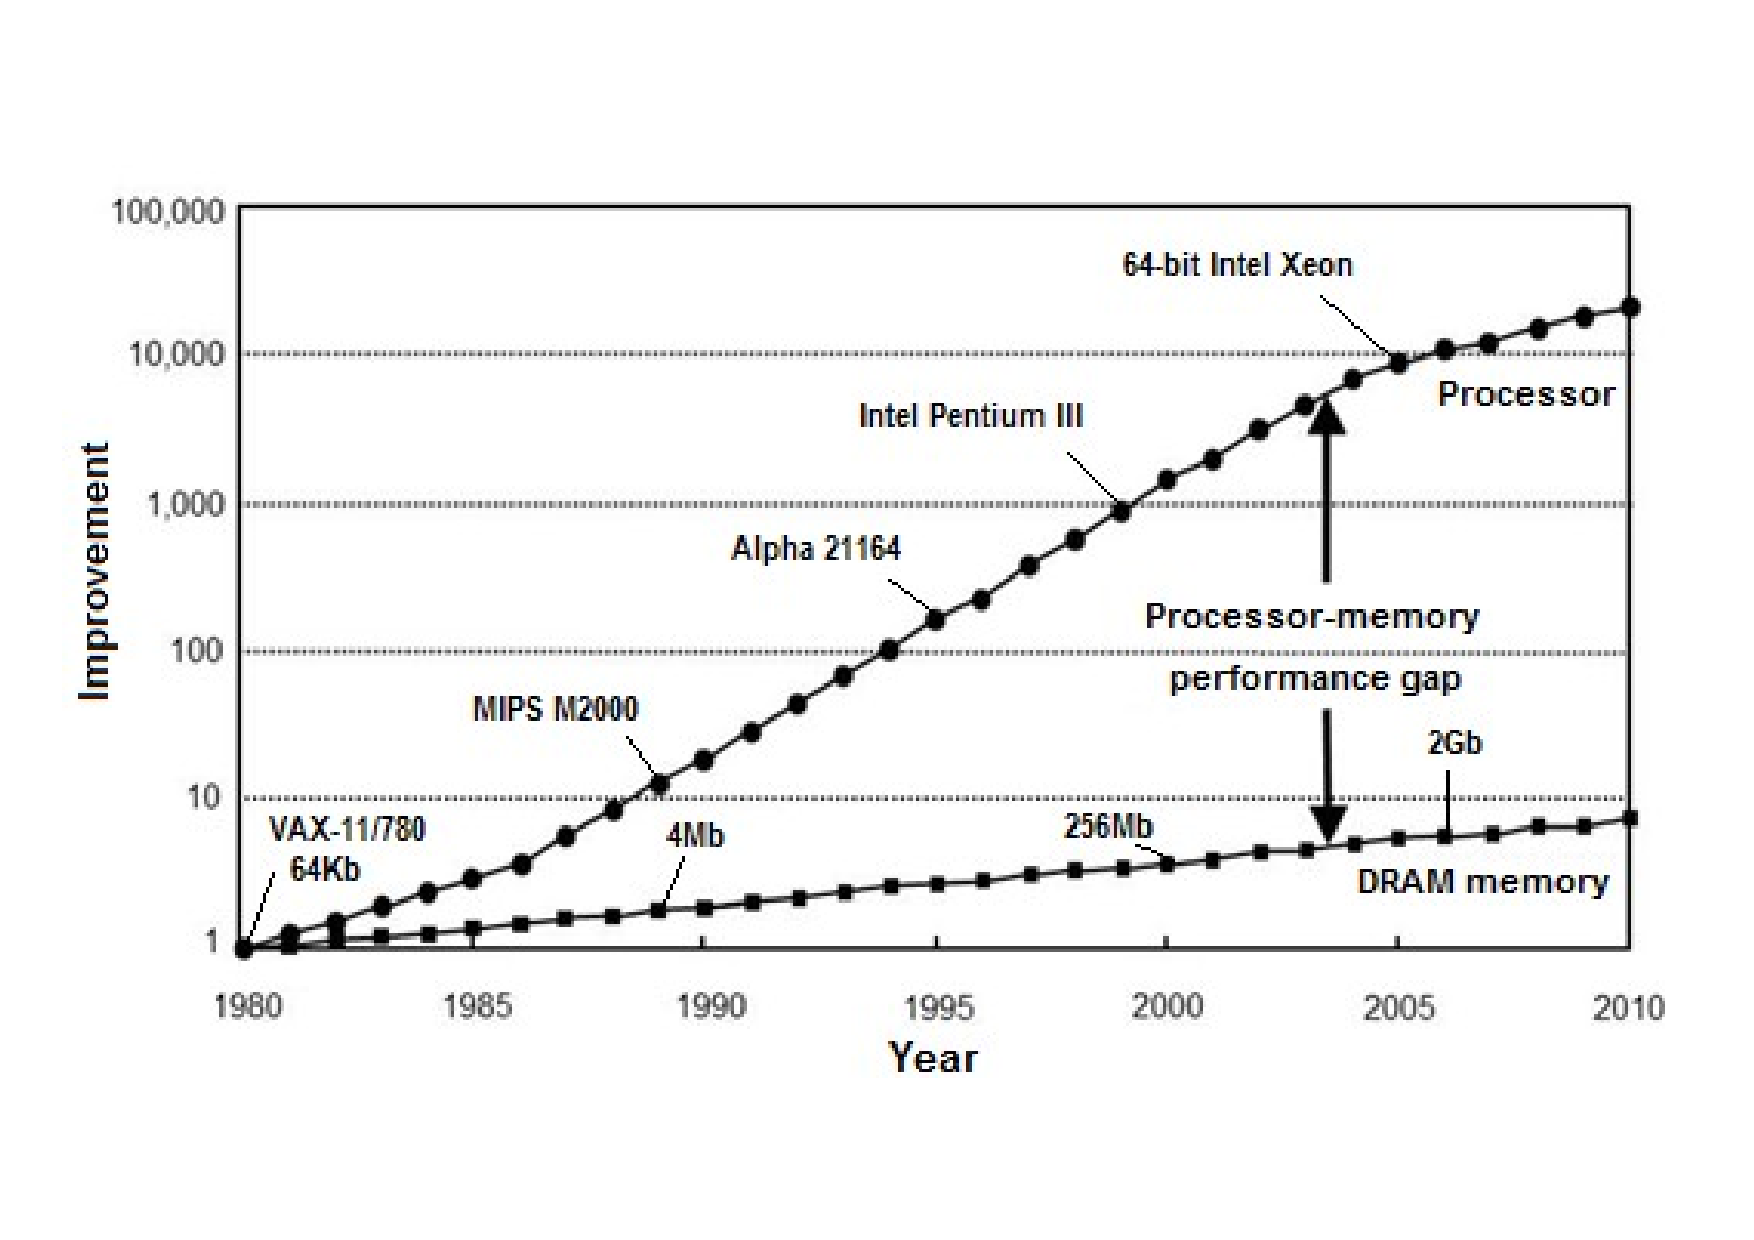
\includegraphics[scale=0.45]{processor_memory_gap.pdf}
	\caption{Processor-Memory gap, figure from \cite{cpu-mem-gap}}
		\label{fig:processor memory gap}
\end{figure}


To reduce the processor-memory performance gap, memory is built up hierarchically, as shown in \cref{fig:memory hierarchy}.
The memory is ordered from fast, expensive and low capacity, which is close to the processor, to progressively slower, cheaper and higher capacity, which is further away from the processor.
The goal of the memory hierarchy is to develop systems that have enough fast memory, CPU cache and DRAM to not slow down the CPU significantly and on the other hand, have as much memory capacity as necessary provided by using hard disks, solid state disk or flash memory without excessive costs.

\begin{figure}[ht]
	\centering
	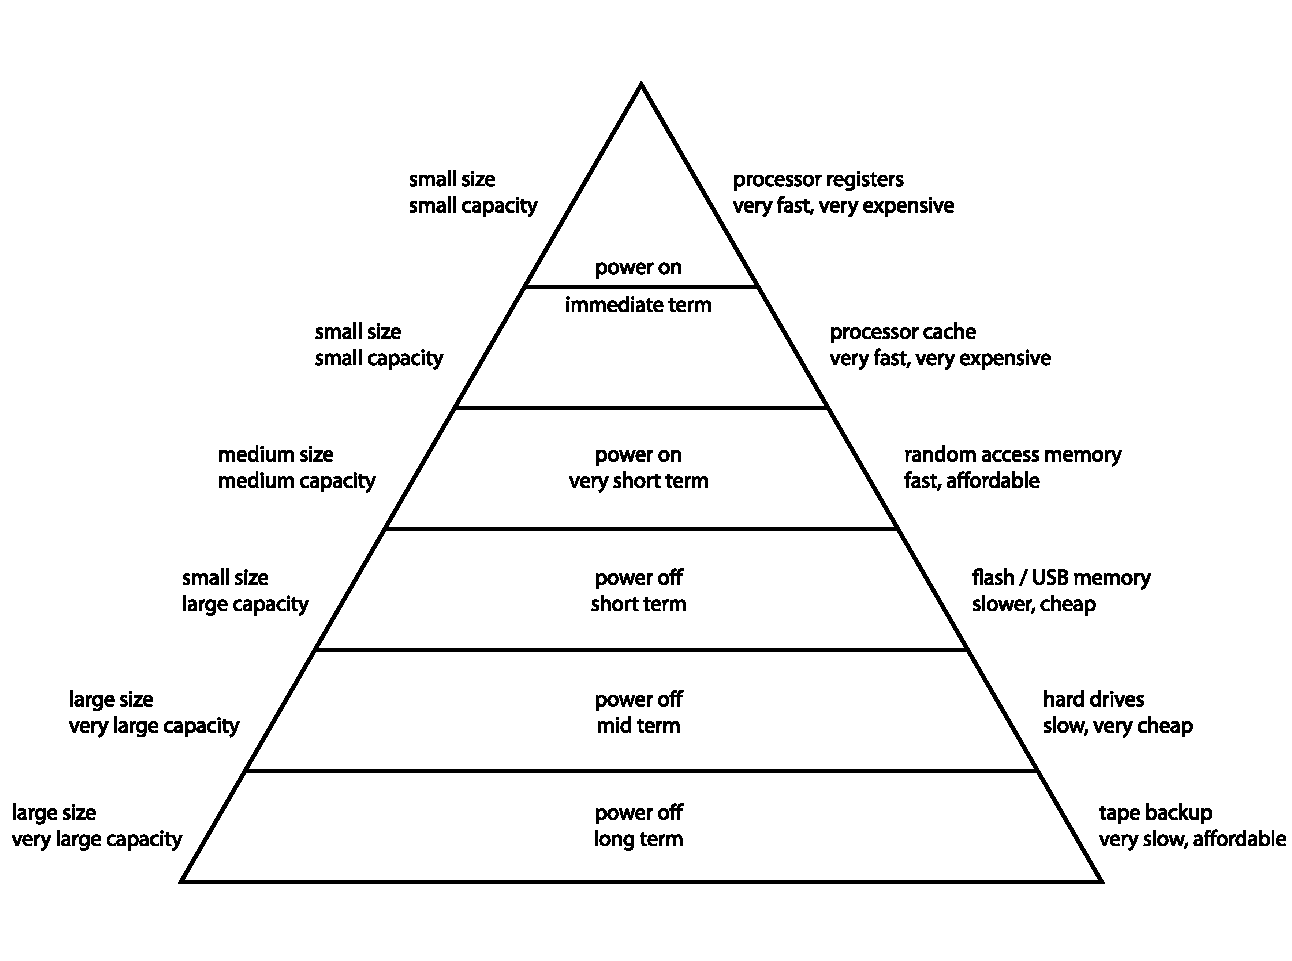
\includegraphics[scale=0.6]{ComputerMemoryHierarchy.pdf}
	\caption{Memory Hierarchy}
		\label{fig:memory hierarchy}
\end{figure}
\todo[inline]{check how to cite online sources, it is from wikipedia https://upload.wikimedia.org/wikipedia/commons/9/9d/ComputerMemoryHierarchy.png}

\section{Caching}
\label{sec:caching}
%Due to the use of a memory hierarchy, caching is used in several places, as shown in table \ref{tab:caching hierarchy} and can either be handle in hardware like the L1 and L2 cache of a cpu-core, in software like a web cache or a combination of both.

Closely related to the memory hierarchy is caching.
Caching refers to a fast and smaller primary memory in front of a larger but slower secondary memory, so that requested data can be served faster from the primary memory instead of fetching the data from the slower memory, which improves latency and throughput and also reduces cost by using less faster memory.
Caching can also mean that data from a remote memory is stored in a local memory for faster access, such as web cache.
The idea of caching is based on the assumption of temporal and spatial locality.
Temporal locality means that a datum accessed in the past is likely to be accessed again, and
spatial locality means that when a datum is accessed, a nearby datum in memory is also likely to be accessed.
To take advantage of spatial locality, blocks of data are considered instead of single datum as seen in \cref{tab:caching hierarchy}.

If we include caching in the memory hierarchy so that each faster memory caches the slower memory below it, we also have a caching hierarchy as shown in \cref{tab:caching hierarchy}.
Caching can be done exclusively in hardware, as is the case with the CPU's L1 and L2 caches, or exclusively in software, as with the Web cache, or in a combination of both, as with the virtual memory of an operating system.
% think that should be formulated differently
Caching is an on going research topic and researches came up with various solution for the different use cases.

\begin{table}[ht]
	\centering
	\begin{tabular}{|p{3cm}|p{3cm}|p{3cm}|p{2cm}|p{3cm}|}
		\hline
		\textbf{Cache Type} & \textbf{What Cached} & \textbf{Where Cached} & \textbf{Latency in cycles} & \textbf{Managed By}\\
		\hline
		Registers & 4-byte word & CPU registers & 0 & Compiler \\
		\hline
		TLB & Address translation & On-Chip TLB & 0 & Hardware \\
		\hline
		L1 cache & 32-byte block & On-Chip L1 & 1 & Hardware \\
		\hline
		L2 cache & 32-byte block & On-Chip L2 & 10 & Hardware \\
		\hline
		Virtual Memory & 4-KB page & Main Memory & 100 & Hardware + OS \\
		\hline
		Buffer Cache & Parts of files & Main Memory & 100 & OS \\
		\hline
		Network buffer cache & Parts of files & Local disk & 10,000,000 & AFS/NFS client \\
		\hline
		Browser cache & Web pages & Local disk & 10,000,000 & Web browser \\
		\hline
		Web cache & Web pages & Remote server disks & 1,000,000,000 & Web proxy server \\
		\hline
	\end{tabular}
	\caption{Caching Hierarchy \cite{7569243}}
	\label{tab:caching hierarchy}
\end{table}

When the cache is full and a cache miss occurs, we have to decide which cache entry tor remove in order to move the requested block into the cache.
This is one of the main problems of caches. If we displace a cache entry that we will need in the near future, we will have an additional cache miss, which we want to avoid.
To decide which cache entry to remove, heuristics, the cache replacement policies, are used.

The advantage of caching is that the latency and bandwidth or both are increased.
But there are also drawbacks.
If we use caching we have redundant data copies in each cache, which on the one hand means increased power consumption.
Each extra copy and move of data consumes additional power.
And on the other hand, if we have redundant data, there is an additional effort to keep the data consistent.
For example, when a cache entry is modified, we need to write the data back to the original location, and we need to prevent multiple tasks from writing to a cache entry at the same time.

\section{Hierarchical Storage Management}

%- some similarities to caching
%- uses migration policies similar to caching policies
%- but instead of copies in faster memory like caching did
%  the data is moved completely
%- data can moved up and downwards the memory hierarchy

Hierarchical storage management (HSM), also known as tiered storage, is a data management method that moves data between levels of the storage hierarchy.
The data is automatically migrated between the storage media based on policies.
Frequently used data is moved up the memory hierarchy to faster and more expensive 
storage media and infrequently used data is moved down to slower but cheaper storage media
 \cite{lugar2001hierarchical}.
Thus, HSM is a trade-off between latency and bandwidth on the one hand 
and cost and capacity on the other.

HSM has some similarities to caching.
Both move data to faster storage based on policies and both have the same goal to improve I/O 
and reduce cost.
But there are fundamental differences between them.
Caching copy the data that is moved to the faster storage and use the copy instead of the original data. 
The original data still continues to reside on the slower storage.
So if the copy in cache is changed, the changes must be written back to the original data.
HSM on the other hand actually moves the data to the faster storage.
Thus, no write back is necessary.

\section{Contribution}
% check if contribution or contributions is right
- new is direct comparison of clock based cache replacement algorithms\\

\section{Outline}
- description of the structure of the following work\\

% 5-10%, ca. 2-5 Seiten 

\chapter{Background}
\label{cha:background}

% darstellen der nötigen Informationen und Arbeiten um die weitere Arbeit verstehen zu können
% nicht zu weit ausschweifen
% 10-20%, ca. 4-10 Seiten

- next chapter gives a short overview of topics necessary to understand the following work\\
- \ref{caching}

\section{$B^{\varepsilon}$-tree}
\label{sec:tree}

% own section for $B^{\varepsilon}$-tree
%The $B^{\varepsilon}$-tree is a write-optimized version of the B-tree, which are widely used for filesystems or databases, with better performance for insert, range queries and key-value updates \cite{bender2015introduction}.
%Unlike the B-tree, the $B^{\varepsilon}$-tree has a buffer for each node, where changes to the subtree associated with the node are stored and
%only when the buffer overflows, the changes are written to the nodes of the subtree, which reduces the number of write operations and the data fragmantation.

The idea for the $B^{\varepsilon}$-tree was introduced by \cite{brodal2003lower} in a study of the trade off between insertions and queries for comparison-based external memory dictionaries.

The basis for $B^{\varepsilon}$-trees is the B-tree, which has good performance on queries but suffers from poor performance on small writes, as shown in \cite{bender2015introduction}, 
because the entire node must be updated for each small write.
However, if we reduce the node size to optimize for small writes, sequential read performance suffers because many smaller nodes have to be fetched from disk instead of fewer but larger ones.

To optimize for both cases, the $B^{\varepsilon}$-tree adds a buffer to each internal node of size $B - B^{\varepsilon} $ with $ 0 \leq \varepsilon < 1$ as shown in \cref{fig:structure B-epsilon-tree}.

\begin{figure}[ht]
	\centering
	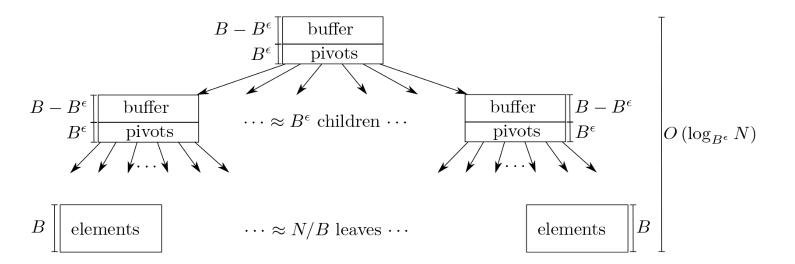
\includegraphics[scale=0.6]{B-epsilon_structure.png}
	\caption{Structure $B^{\varepsilon}$-tree from \cite{bender2015introduction}}
		\label{fig:structure B-epsilon-tree}
\end{figure}

As new data is inserted into the $B^{\varepsilon}$-tree, the data is written to the buffer of the root node as "insert message".
Only when the root node's buffer is full, a batch of messages is flushed down the tree, preferably to the node with the most pending messages. 
If a node needs to be split, the buffer is also split between the new nodes.
When the insert message arrives at a leaf node, the data is added to the leaf.

This behavior leads to better insertion performance than B-trees, since insertion always occurs at the root, no searching for the correct insertion point is required, and  
the actual writing of data is delayed in batches only when enough changes have accumulated in a buffer.
On deletion a "tombstone message" will be insert into the tree and will be flushed down the tree to a leaf, like an insertion message.

For queries, in the $B^{\varepsilon}$-tree, we also need to check buffer on the way to the leaf nodes to see if there are any relevant messages.
These messages must be processed, but that does not mean they are flushed down immediately, this can happen later.

So the $B^{\varepsilon}$-trees achieves similar asymptotic I/O cost for queries but is better for insertions compared to B-trees.
\todo[inline]{write a bit more detailed about this}

\section{Copy on Write}
\label{sec:copy on write}

- should be mentioned because it important part of haura and $B^{\varepsilon}$-tree\\
- used for easy creation of snapshots \\
- described in \cite{patterson1995informed}\\

\section{Haura}
\label{sec:haura}

Haura is a research storage stack written primarily in Rust.
Unlike traditional file systems, Haura runs in user space rather than kernel space.
Also, Haura uses a key-value and object interface rather than the usual POSIX interface.
It can be used either directly by an application, in which case Haura runs in the process context of the application, or
use JULEA as a wrapper for Haura.
JULEA then runs the Haura instance detached from the user applications, which means that the user application can be terminated or new applications can be created as long as JULEA is running, resulting in more flexibility compared to direct use.

\todo[inline]{insert schemes from Haura docu for better understanding}
\todo[inline]{insert link to Haura docu as source}

The development of Haura started to compare $B^{\varepsilon}$-tree to ZFS and ext4 filesystem \cite{wiedemann2018modern}, where the Haura stack
achieved an improved write performance especially for small random write workloads and better sequential throughput.
Then Haura would be extended by \cite{hoppner2021design} to support multiple storage levels
The work of \cite{hoppner2021design} extended Haura with an object storage interface and the support of multiple storage levels while preserving the benefits of the $B^{\varepsilon}$-tree.

As pointed out by \cite{wunsche2022data} the advantage of Haura is that all levels which a relevant to implement and optimize a storage stack a combined in a single code base, so that it is easy change subsystems and test different approaches.
Haura is structured in layers as shown in \cref{fig:structure Haura}.

\begin{figure}[ht]
	\centering
	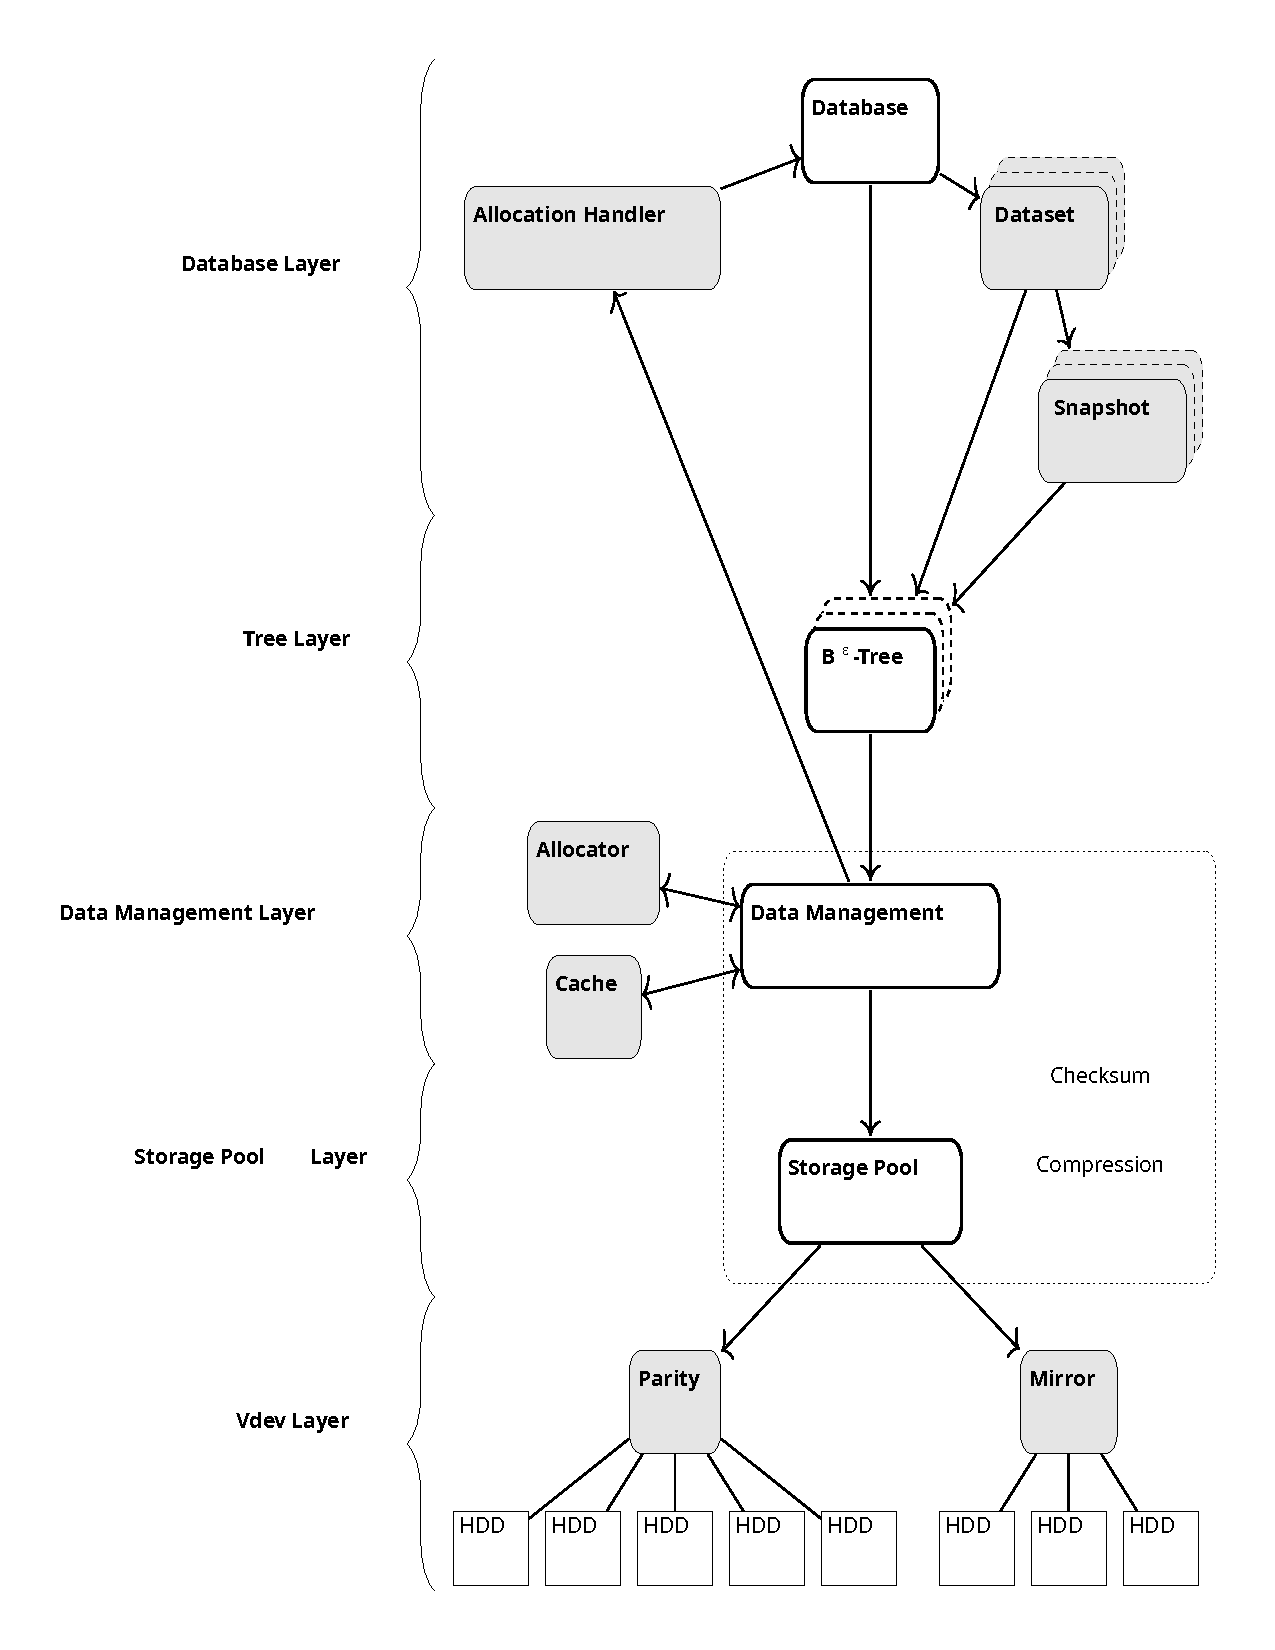
\includegraphics[scale=0.4]{overview_haura_level.pdf}
	\caption{Structure Haura \cite{wiedemann2018modern}}
		\label{fig:structure Haura}
\end{figure}



At the top is the \emph{Database Layer} which manages multiple datasets and snapshots. Each dataset provide a key-value interface, snapshots only read-only key-value interface. Also for each dataset exists an own $B^{\varepsilon}$-tree and  a root tree which saves the allocation bitmaps and metadata.

The next layer, the \emph{Tree Layer} manages the $B^{\varepsilon}$-trees.
The \emph{database layer} sends messages to the $B^{\varepsilon}$ trees consisting of key-value or key-message pairs that the $B^{\varepsilon}$ trees process. A message for key-message pair can contain arbitrary data or apply arbitrary code on data.
Key-value pairs are stored in leave nodes and key-message nodes are stored in inner nodes of the tree.
Each node is an object for the \emph{Data Management Layer} and is tracked individually.

The \emph{Data Management Layer}(DML) manages objects for the \emph{Tree Layer} and \emph{database layer} which means cache objects in memory, 
track modifications to objects and write-back modified objects.
Main part of the DML is the Data Management Unit (DMU).
The DMU is shared by all trees and ensures that no irregular state can be reached.
It takes care of critical disk management such as block allocation.
In addition, the DMU manages the cache, which is the main topic of this work.

The \emph{Storage Pool Layer} is an abstraction over the used storage hardware.
Furthermore the storage is divided in to tiers from \emph{Fastest}, \emph{Fast}, \emph{Slow} to \emph{Slowest}.
The user can decide how the used hardware falls into these tiers. Also, not all tiers need to be used.

The last layer, the \emph{Vdev Layer}, is responsible for actually reading and writing data from the disks.
Single disk, multiple disks or RAID-like configurations can be used.

\section{Cache Replacement Policies}
\label{sec:cache replacement policies}

- introduction text needed
- make reference to introduction, mentioned caching there

\subsection{Optimal Cache Replacement Policy}
The theoretically optimal cache replacement policy is Bélády's algorithm (also known as OPT or clairvoyant algorithm) \cite{belady1966study}.
This algorithm always evicts the cache entry whose next use is furthest in the future.
The problem is that this information is usually not available during runtime, but only after an application has ended.
Even though this optimal algorithm is not used in any real system, it is useful for theoretical comparison with other 
Cache replacement algorithm.
Furthermore, many improved cache replacement strategies attempt to approximate the optimal cache replacement strategy.
Next, I will present three early developed cache replacement policies that are still in use, but also form the basis for further improved policies.


\subsection{FIFO}
% could be mention the time complexity

First in, First out (FIFO) is a very simple cache replacement policy.
All cache entries are stored in a queue based on a single linked list.
Each time a cache entry needs to be evicted, the entry that has been in the cache the longest is removed.
This is the entry at the front of the queue, and any new entry is inserted at the back of the queue. Both operations have a constant O(1) time complexity.
So before a cache entry will be evicted, it has to go through the entire queue.

The advantages of FIFO are that it is simple and easy to implement.
Also no further metadata needs to be saved for each entry so that on each cache hit we do not need to update the queue.
This is advantageous when multiple tasks can access the cache, because then 
we don't need locks to managed the access.
Furthermore, the absents of metadata and additional data structures make FIFO better suited for cases where strict size constraints must be met. 
We will see later that other cache replacement algorithms have ghost queues or multiple queues that can shrink and grow. So the size 
of a FIFO cache is predictable, or rather, there is a minimal memory overhead for FIFO compared to other replacement strategies.

However, the assumption that the entry with the longest time in the cache is always the best candidate for removal is far too 
simplistic and often more advanced cache replacement algorithms significantly outperform FIFO \cite{van1992lru}.
One reason for this is that it does not distinguish between frequently or recently accessed entries that should remain in the cache, and new entries that are rarely accessed again. Ever entry is treated equally. This can lead to many unnecessary evictions.
Another disadvantage is that FIFO suffer from the Bélády's anomaly \cite{10.1145/363011.363155} which means that an increased cache can lead to an increased cache miss rate, Least-Recently-Used replacement policy for example doesn't suffer from the Bélády's anomaly.
%thrashing could be insert as disadvantage 

\subsection{Least Recently Used}
Another widely used cache replacement policy is Least Recently Used(LRU).
It dates back to at least 1965 \cite{denning1980working} and is probably even older.
The idea of LRU is that whenever an entry needs to be evicted, the entry that has not been accessed for the longest time is evicted.

All cache entries are stored in a priority queue, usually implemented as double linked list, sorted by there last access time.
Each new entry is insert at the front of the priority queue and the entry at the back of the priority queue is always selected for eviction.
In case of a cache hit, the entry that is in the priority queue is placed at the front of the queue.
In general, it is too costly to keep track of the last access time, and only approximate values, such as age bits, are used instead.

Compared to FIFO, LRU performs equal or better \cite{van1992lru}.
The reason for this is that in many cases the access distribution is skewed, so that a small number of cache entries are accessed more frequently than the others.
As a result of this, the entries that are frequently accessed are pushed to the top of the priority queue and thus are rarely evicted from the cache.

One disadvantage, compared to FIFO is, that we have the overhead of additional metadata, the access time or the approximation of it, for each cache entry.
Thus, LRU requires more memory to store the same number of cache entries.
Furthermore, cache hits also cause additional overhead. 
This is because a cache hit changes the order of priority queue.
Especially in cases where multiple tasks use the cache, this must happen behind a lock to ensure consistency.
This can lead to additional waiting times for multiple tasks that have to wait until the cache hit has been processed.

Another disadvantage is that LRU does not use frequency information.
Thus, an entry that has been accessed frequently but not recently could be evicted for a entry that has been accessed infrequently but recently.
An example for that is are looping or scanning pattern, like iterating over an array or searching a file.
Then a burst of often only once accessed entries, can lead to the eviction of entries which are accessed more frequently and should stay in cache.

Despite these drawbacks, LRU is widely used.
This is because it is still a simple policy that is easy to implement.
It has good performance with limited additional overhead and works well with strong locality and skewed access distribution.

\subsection{Least Frequently Used}

% maybe a different start for this chapter?
The Least Frequently Used(LFU) policy is based on the idea that a cache entry that has been used frequently in the past will also be used in the future.
Thus, when a cache miss occurs, the least frequently accessed entry is evicted.
In case more then one entry have the same access count we have to use FIFO or decide randomly which entry has to be evicted.

All cache entries are stored in a priority queue, usually implemented as double linked list or a min-heap, sorted by there access frequency.
The entry with the lowest frequency in cache is at the back and the entry with the highest frequency in cache is at the front of the priority queue.
As metadata, we have a counter assigned for each cache entry.
On a cache hit the counter for the entry will be incremented and the entry could change his position in the priority queue.

The advantage of LFU is that frequently accessed entries remain in the cache and with constant
access distributions, LFU has the best cache hit ratio \cite{einziger2017tinylfu}.
But LFU has some  serious drawbacks.
First, the overhead for maintaining the metadata is higher than for LRU and FIFO.
Also, as with LRU, there is a problem with lock contention when the priority queue is updated on a cache hit.
And second, the access frequency and distribution is not constant over time.
For example, if a cache entry is accessed frequently during the startup of an application but not thereafter, it may take a long time for the entry to be removed from the cache.
The problem in this case is that LFU do not use recency information.
There two main strategies used to make LFU more adoptable for this case.
The first is aging, which means that the access counter for each entry is decreased after  a certain amount of time.
And the second strategy is to use only a fixed time window to count accesses and after the window restart each access counter \cite{karakostas2000practical}.

LFU is not used as often as LRU.
Since it is more complex without performing better in most cases.
However, one important area where LFU outperforms LRU is web caches.
This is because web caches have a highly skewed access distribution with low locality and  
many entries accessed only once, \cite{mahanti2000traffic}.

\section{Improved Cache Replacement Policies}
\label{sec:improved cache replacement policies}

All cache replacement policies presented in the last section have significant drawbacks.
Bélády's algorithm must know the access pattern in advance and is only of theoretical value.
FIFO suffers from the Bélády's anomaly and has higher miss rates then the other policies.
LRU has problems with access patterns that have only weak locality, such as loop or scan patterns.
And LFU is has to much overhead and only outperforms LRU for highly skewed access patterns. 

To further enhance cache performance, several additional cache replacement policies have been developed and
most of these policies are based on the policies presented so far.
The strategies for improvement can be divided into 4 categories,
(1) explicit user-level hints, (2) using a deeper history information
(3) detection of access patterns (strategies (1)-(3) from \cite{10.1145/511399.511340})
and (4) the use of ml-techniques, which we will discuss in more detail below.
\todo[inline]{use listing, instead of numbers in text}

\subsection{Explicit User-Level Hints}

The first improvement strategy is through user-level hints.
This idea was proposed by \cite{cao1994application} and \cite{patterson1995informed}.
The idea is that the user provides hints about which cache entries have a low probability of being accessed in the near future.
The problem with this approach is that the user must understand the access pattern in order to provide appropriate hints, which increases the programming effort \cite{10.1145/511399.511340}.
Therefore, user-level hints can be a solution in special cases,
but they are less suitable as a general cache replacement policy.

\subsection{Utilizing Deeper History Information}

The second strategy is to use more history information.
LRU in particular has the problem that it uses very little information, only the last reference, to decide which entry to evict.

One example for this approach is LRU-K proposed by \cite{o1993lru}.
LRU-K works similar to LRU, but instead of using only the last reference, like LRU,
the Kth-to-last reference are used for the eviction decision. 
Usually $K = 2$ is chosen, for simplicity and better adaptability to different access patterns then $K > 2$.
The advantage of LRU-K is that it is better suited for loops and scanning access patterns.
This is because cache entries that are referenced only once are removed from the cache more quickly than with LRU.
However, LRU-K has the same major problem as LRU, which is the cost associated with using a priority queue.
Any manipulation of the priority queue requires $O(\log(n)$ operations \cite{10.1145/511399.511340}.

The 2Q policy of \cite{shasha19942q} attempts to achieve the same performance as LRU-K, but without the $O(\log(n)$ complexity of using a priority queue.
Instead of using just one queue, 2Q uses two queues.
An FIFO queue \emph{A1} and an LRU priority queue \emph{A$_m$} as main cache.
Also, the \emph{A1$_{in}$} is split into \emph{A1$_{in}$} for entries that actually exist in the cache and \emph{A1$_{out}$} for entries where only the reference is stored.
If a cache hit occurs and the entry is in \emph{A1$_{out}$}, the entry is promoted to the main cache \emph{A$_m$}.
If there is a cache hit in \emph{A1$_{in}$}, the entry remains in \emph{A1$_{in}$}.
Also, for a cache hit in \emph{A$_m$}, \emph{A$_m$} behaves like a priority queue and places the entry at the beginning of \emph{A$_m$}.
The entry for eviction is either the front entry of the \emph{A1$_{in}$} queue, if the length of the \emph{A1$_{in}$} is greater then a certain threshold, or the tail of the 
\emph{A$_m$} otherwise.
Like LRU-K, 2Q is better suited for looping and scanning access patterns.
This is because only once referenced entries leave the cache quickly.
However, the advantage is that 2Q has a constant time overhead.
The disadvantage on the other hand is that the 
length of the \emph{A1$_{in}$} and \emph{A1$_{out}$} queues is predefined.
But these parameters needs to be tuned for each use case to achieve optimal performance.

Another example is Least Recently/Frequently Used(LRFU) policy \cite{lee2001lrfu}.
LRFU combines LRU and LFU methods by tracking the frequency and reference for each entry and using a weighting factor $\lambda$ to decide which is more important.
The problem with this approach is that the $\lambda$ is fixed.
It is therefore not adaptable to changing access patterns.
Furthermore, the $\lambda$ parameter is highly dependent on the hardware used and the access pattern.
We must therefore determine the correct $\lambda$ for each use case.
Therefore, LRFU is also not suitable as a general cache replacement algorithm.

\subsection{Detection and Adaption of Access Patterns}

The third strategy is to identify specific access patterns in the history information for certain entries, based on either temporal or spatial locality, and treat these entries differently from the other entries.

An example of this strategy is Low inter-reference Recency Set (LIRS) \cite{10.1145/511399.511340}.
Instead of using recency directly like LRU, LIRS uses inter-reference recency (IRR), also called reuse distance.
IRR refers to the number of other entries accessed between two consecutive references to a given entry.
This allows the cache entries to be divided into either hot or cold entries.
Hot entries have a low inter-reference recency and are likely to be accessed again in future.
They should therefore remain in the cache.
And cold entries on the other hand have a hight inter-reference recency and are unlikely to be accessed again in future, which means that they can be easily removed without causing many additional cache misses.
So we divide the cache capacity into a smaller part for hot entries and a larger part for cold entries.
Furthermore, a variable number of non-resident cold entries can be stored.
The non-resident cold entries are necessary to track the IRR.
LIRS uses one LRU priority queue and one FIFO queue, as shown in \cref{fig:lirs queues}.
The LRU-queue stores all hot, all resident cold and non-resident cold entries.
The FIFO queue stores only the resident cold entries and is used to find the entry to be evicted.
Instead of tracking the IRR directly, the position between entries in the LRU priority queue is used to determine the IRR and to 
to control when a cold entry converts to a hot entry and vice versa.
The advantage of LIRS is that it eliminates the weakness of LRU for weak locality workloads with relatively low overhead.
The disadvantage is that we still have to predefine the ratio between the capacity for hot and cold entries.

\begin{figure}[ht]
	\centering
	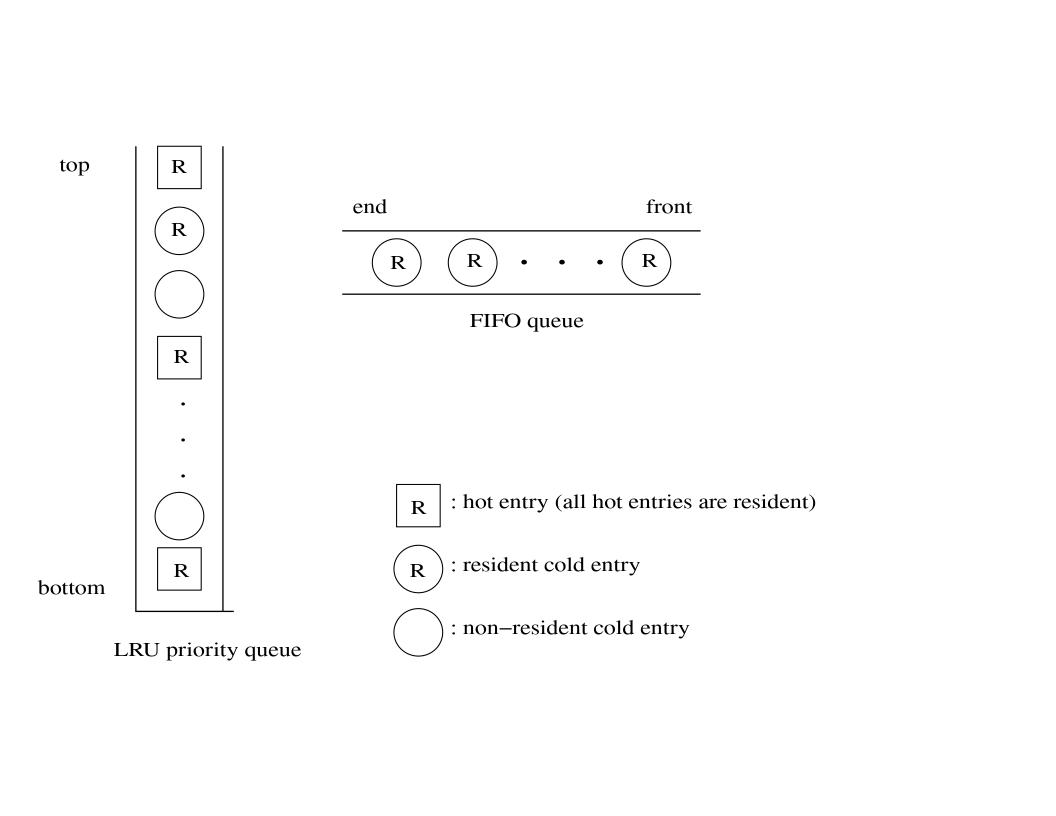
\includegraphics[scale=0.5]{lirs_queues.jpg}
	\caption{Shows the LRU stack and FIFO queue used for LIRS, original from \cite{10.1145/511399.511340} labeling  altered.}
		\label{fig:lirs queues}
\end{figure}


Another example is Adaptive Replacement Cache (ARC) \cite{270366}.
ARC uses two LRU priority queues, $L_1$ for entries entries who are accessed only once in the recent past and $L_2$ for entries accessed at least twice in the recent past.
So $L_1$ measures recency and $L_2$ the frequency.
For a cache with the capacity for $c$ number of entries and each queue can also hold $c$ number of entries.
The cache saves $2c$ entries, of which $c$ are non-resident entries.
To achieve adaptability the number of resident entries for each queue is not fixed and changes according to the workload.
Each time a cache hit occurs on a non-resident entry in one of the queues, the number of resident entries for that queue is increased
depending on the ratio between the number of non-resident entries of each queue.
Also, whenever a cache hit occurs on an $L_1$ entry, whether resident or non-resident, it is removed from $L_1$ and added to $L_2$.
So depending on the workload and thus the non-resident entries being accessed, ARC behaves more like LRU or LFU.
The significant advantage of ARC is that it is adoptable and has no parameters like LIRS or 2Q that need to be manually optimized.
Also the the space overhead is still low with only 0.75 percent of the cache size \cite{megiddo2004outperforming}.

\subsection{Using Machine Learning}

The last strategy has emerged only in recent years and seeks to incorporate machine learning techniques to learn the underlying access pattern to increase the hit rate.
This can be done either by online learning, where learning occurs during execution and is adoptable to changing workloads, or by offline learning, where parameters are learned before execution using a predefined data set.

An example of this strategy is fuzzy page replacement algorithm by \cite{akbari2020page}, which uses
fuzzy c-means, an unsupervised machine learning technique, to find clusters in all cache entries based on the frequency, recency and time difference between two consecutive accesses for each entry.
Each time an entry needs to be evicted, the entry with the greatest distance to all cluster centers is evicted.

Another example is proposed by \cite{choi2022learning} which uses Seq2Seq network, a type of recurrent neural network designed for handling sequence data.
The history of the last accessed cache entries is used to predict a sequence of the future accesses.
The predicted sequence is then applied to conventional cache replacement algorithms, like LFU or LRU, to prevented unnecessary evictions. 


\section{Summary}
\label{sec:summary}

- heuristics mostly work for the intended cases but have problems in other cases, give examples for that\\
- machine learning the new hype\\
- many new papers for this topic \\
- have the chance to actual be adoptable to all possible access patterns and significant increase miss ratio for wide array of use cases \\
- but can have higher overhead compared to simple heuristics\\
- open question which approach is best for machine learning techniques.

\chapter{Related Work}
\label{cha:related work}
% es werden Arbeiten presentiert bzw. meine Arbeit mit diesen vergliechen
% was hab ich anders gemacht bzw. wie sind andere Autoren an das Thema ran gegangen
% 5-10%, ca 2-5 Seiten

\section*{It's Time to Revisit LRU vs FIFO by \cite{eytan2020s}}

Earlier studies between LRU and FIFO performance are probably not sufficient for newer use cases such as web cache, ML ...
Because the workloads and the sizes of caches changed dramatically over time.
The general guide line LRU is better then FIFO isn't true in all cases.
When the cache is to big to hold it completely in main memory FIFO is better because only the end where the eviction happens and the start of the FIFO queue need to be in main memory. So the simpler structure is more suitable in this case than LRU.
LRU still better choice when the latency of memory is the dominating factor.

\section*{FIFO can be Better than LRU: the Power of Lazy Promotion and Quick Demotion by \cite{yang2023fifo}}

Although FIFO is a simple to implement cache replacement algorithm with O(1) complexity for insertion and removal and therefore provides good throughput.
The major drawback was the lower hit rate compared to LRU-based algorithms.
The paper by \cite{van1992lru} proofed that LRU is better under the assumption of an independent reference model.
But this paper \cite{yang2023fifo} shows that FIFO can achieve comparable performance to modern LRU based cache replacement algorithms.
This study uses very large data sets/traces from different use cases.
The key to achieve this is the use of Quick Demotion and Lazy Promotion.
Quick Demotion is based from the observation that often recently insert entries also leave the cache quickly. So these new entries are insert in a smaller FIFO queue, 10\% of cache and also a ghost queue for evicted entries is used which only saves metadata not the actual entries. So if a new entries leaves the QD-queue it will be insert to ghost queue. If then an access to the same entry happens where the entry is in ghost the entry will be insert to main cache.
Quick Demotion can be combined with different cache replacement algorithms not just FIFO.
To some extend some cache replacement algorithms have some kind of  Quick demotion incorporated. 
Lazy Promotion tries to maintain hot entries in cache with minimal overhead.
To achieve this Promotion only happens at eviction not at access like LRU which decrease the handling of metadata. Example for this would be 2-bit Clock algorithm.
This approach could be easy implemented by adding Quick Demotion and use 2-bit Clock as main cache.
Different implementations for QD and LP possible can lead to many different modular algorithms. 

\section*{FrozenHot Cache: Rethinking Cache Management for Modern Hardware by \cite{qiu2023frozenhot}}

This is a new cache replacement algorithms based on list.
The cache is divided in a frozen cache and a dynamic cache.
The frozen cache(FC) is for hot entries and if fixed to reduce latency by removing eviction and locking for those entries. 
The Dynamic cache(DC) on the other hand is used to achieve adaptability.
Rebuilding of the frozen cache happens periodically.
It is possible to combine this approach with different list based caches with minimal effort.
So this is a cache better suited for multi-threading.

\section*{TinyLFU: A highly efficient cache admission policy by \cite{einziger2017tinylfu}}

This is a LFU based cache replacement algorithm which uses a Bloom-Filter to approximate the frequency information for the cache entries with a relatively small memory usage.
So even for large caches which can't be entirely in RAM the Bloom-Filter is small enough to fit in to RAM.
It is based on the assumption of a skewed accesses distribution like zipfian.
Also a small window, a FIFO queue is used to bring requested entries into the cache and then
with the help of the frequency statistic in Bloom-filter the algorithm decide if it is better to bring the entry to the main cache or not. Main cache could be different caching algorithm.
So TinyLFU has something like a Quick Demotion which means rarely used entries leave the cache quickly or are not transferred to the main cache at all.
TinyLFU is intended for relatively large caches probably doesn't work as well on small caches ot the extra cost for bloom-filter are not justified.

%clock-pro+ could also be a candidate for related work

\section*{Summary}

\chapter{Design and Implementation}
\label{cha:design and implementation}
% Design and Implementation fehlen?! als Kapitel
% 25-35%, ca 10-14 Seiten

% see if I want to mention copy-on-write in background Haura or somewhere else

In this chapter, we describe the cache replacement strategies that we implemented in Haura 
and also the changes we had to make to Haura to implement them.
First, we consider the DML state cycle (\cref{sec:dml state cycle}), 
since the behavior of the DMU, and thus the cache, follows it.
After that, we are looking at the cache trait, the interface that any cache implementation must follow.
Lastly, we examine all the cache replacement strategies that have been implemented.
Starting with CLOCK, which was already implemented,
followed by the newly implemented cache replacement policies GCLOCK, CLOCK-Pro and ML-CLOCK.


\section{DML State Cycle}
\label{sec:dml state cycle}

The task of the DML is to manage objects for the tree layer. This includes reading objects from the disk, storing them in the main memory, tracking changes and writing them back.
This is done by a single DMU which is shared between all trees of the upper layer.
Thus, the DMU is also responsible for the management of the cache.

To accomplish all this, objects must be uniquely identifiable.
All unmodified and all on-disk DML objects are identified by an \emph{ObjectPointer}.

\bigskip

\begin{lstlisting}[language=Rust,mathescape=true,caption=ObjectPointer struct ,label=lst:ObjectPointer struct]
pub struct ObjectPointer<D> {
    pub(super) decompression_tag: DecompressionTag,
    pub(super) checksum: D,
    pub(super) offset: DiskOffset,
    pub(super) $\textcolor{black}{\texttt{size}}$: Block<u32>,
    pub(super) info: DatasetId,
    pub(super) generation: Generation,
}
\end{lstlisting}
% pub(super) makes an item visible to the parent module. This is equivalent to pub(in super).

The struct fields \texttt{offset}, \texttt{size}, \texttt{checksum} and \texttt{decompression\_tag}, in \cref{lst:ObjectPointer struct}, are used to read an object from disk and decompress it.
The \texttt{info} field can be used to store additional tags for an object.
And the last field \texttt{generation} is used to track the age of an object.

The DML objects can be called by their unique \emph{ObjRef}.
This reference, shown in \cref{lst:ObjRef enumeration}, equals to the state of an object at the last access.
Thus, four states are possible unmodified, modified, in write back or incomplete.
If an object is unmodified, it can be identified by his \emph{ObjectPointer} and
when the object is either modified or in write back, objects are given a unique \emph{ModifiedNodeId} for identification.
The incomplete state, as seen in \cref{lst:ObjRef enumeration}, can only be reached when an object is deserialized from disk.
If the DMU encounter an incomplete object during runtime, Haura panics and crashes.

\bigskip

\begin{lstlisting}[language=Rust,mathescape=true,caption={ObjRef enumeration, parameter P equals \&ObjectPointer<D>},
	label=lst:ObjRef enumeration]
pub enum ObjRef<P> {
    Incomplete(P),
    Unmodified(P, PivotKey),
    Modified(ModifiedObjectId, PivotKey),
    InWriteback(ModifiedObjectId, PivotKey),
}
\end{lstlisting}

\begin{figure}[ht]
	\centering
	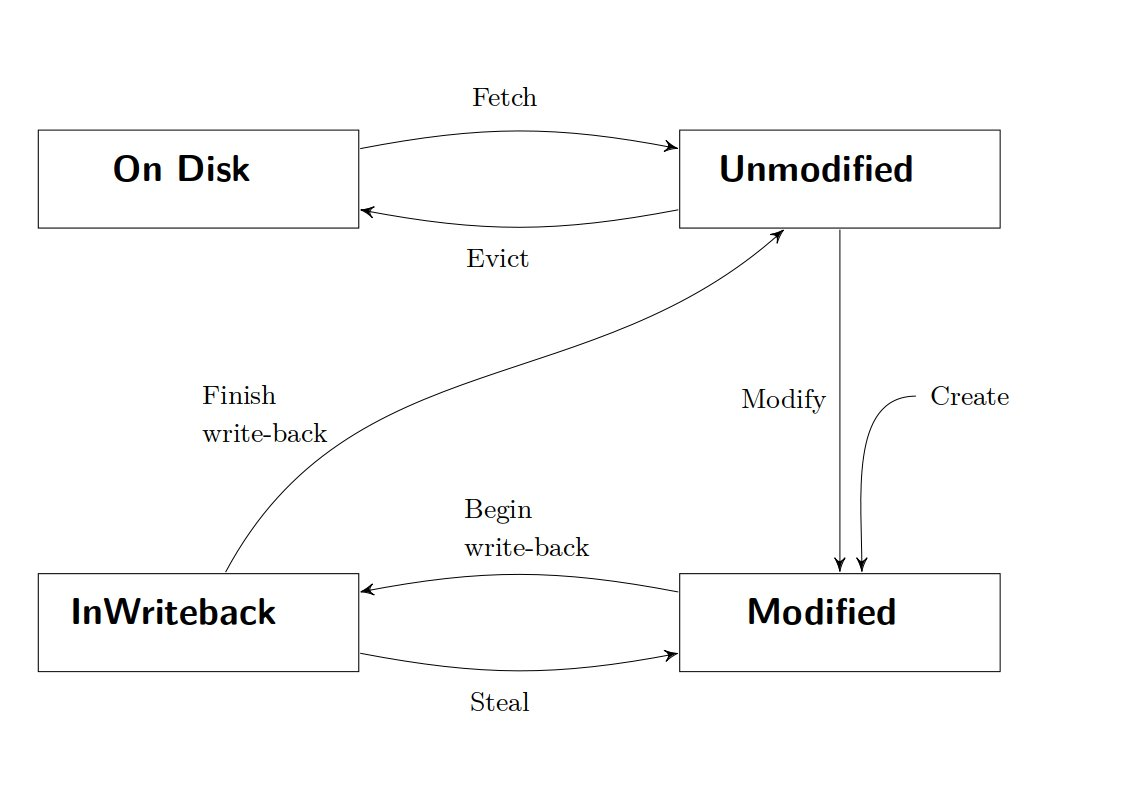
\includegraphics[scale=0.4]{DML_state_cycle.jpg}
	\caption{DML state cycle, \cite{wiedemann2018modern}}
		\label{fig:DML state cycle}
\end{figure}

The DMU manages the cache and the states of each \emph{ObjRef} as shown in \ref{fig:DML state cycle}.
The cycle starts with the creation of an object in modified state. When the DMU starts the write back of the object, the state
is changed to in write back state.
If the object is modified during write back through the steal function, it change the state back to modified.
When the write back is finished the object state change to unmodified.
An unmodified object can either change the state to modified if the object has been modified or evicted from cache to disk.
And lastly, any object on disk can be fetched in cache and will be in unmodified state.

For the cache, all objects are managed with an unique \emph{ObjectKey}, as shown in \cref{lst:ObjectKey enumeration}.
These \emph{ObjectKey} are  from the \emph{ObjRef} for each cache entry.
Objects in incomplete state are not stored in cache.

\bigskip

\begin{lstlisting}[language=Rust,mathescape=true,caption=ObjectKey enumeration,label=lst:ObjectKey enumeration]
pub enum ObjectKey<G> {
    Unmodified { offset: DiskOffset, generation: G },
    Modified(ModifiedObjectId),
    InWriteback(ModifiedObjectId),
}
\end{lstlisting}

\bigskip

\section{Cache Trait}
\label{sec:cache trait}

The DML state cycle and the fact that the cache is managed by the DMU place additional demands on the cache.
We see this in the cache trait, \cref{lst:simplified Cache trait}.

The first difference is that we have an explicit evict function. In most cache implementations, evict is a private function that the cache itself calls.
In our case, however, the DMU must call the evict function, not the cache itself.
Furthermore, the evict function must take into account that there are cache entries that 
are pinned i.e. in write back or modified state and therefore cannot be removed from the cache.
Also, the DMU can remove specific cache entries, \cref{lst:simplified Cache trait} line 6 and line 7.
The \texttt{remove}()-function for unmodified entries and \texttt{force\_remove}() for pinned entries.

\bigskip

\begin{lstlisting}[language=Rust,mathescape=true,caption={simplified Cache trait without type aliases, generics, function parameters and function return types},label=lst:simplified Cache trait]
trait Cache {
    fn new();
    fn contains_key();
    fn get();
    fn get_mut();
    fn remove();
    fn force_remove();
    fn change_key();
    fn force_change_key();
    fn evict();
    fn insert();
    fn iter();
    fn $\textcolor{black}{\texttt{size}}$();
    fn capacity();
    fn stats();
    fn verify();
}
\end{lstlisting}

The second difference is that it must be possible to change the key for cache entries.
Because an object in cache can change his state 
Therefor we have two functions, \cref{lst:simplified Cache trait} line 8 and line 9. 
Again two functions for unmodified and pinned entries.

Another difference is that the cache must be able to handle cache entries of any size.
The handling of cache entries of arbitrary size is managed by the DMU.
Each fetched entry is always inserted into the cache, and then the eviction function is invoked until the cache capacity is again below the specified cache size.
So the cache size is a soft limit that can be temporarily exceeded, not a hard limit, which would mean that the eviction function is called
is called before inserting so that the cache size is never exceeded.

Furthermore, we have added the \texttt{get\_mut}()-function, \cref{lst:simplified Cache trait} line 5, 
since the \texttt{get}()-function does not allow that the state of the cache changes, respectively atomics are used and thus a read-lock is sufficient.
But for ML-CLOCK it is needed to change the cache and atomic operations cannot be used.
Therefore we implemented \texttt{get\_mut}()-function which uses an exclusive write-lock.

\section{Implemented Cache Replacement Policies}
\label{sec:implemented cache replacement policies}

In this Section, we examine the implemented cache replacement policies.
We have limited ourselves to clock based cache replacement policies since they have a lower overhead compared
to most list-based cache replacement policies.
Since clock-based replacement strategies try to do as little work as possible when cache hits occur and 
do most of the work during the eviction of an entry, which should be infrequent.

We followed the improvement strategies from the \cref{sec:improved cache replacement policies}
in selecting the cache replacement policies to implement.
The CLOCK policy was already implemented and is an approximation of LRU.
The next policy we consider is GCLOCK, a generalization of CLOCK that uses more history information.
CLOCK-Pro is an example of a cache replacement policy that recognizes access patterns.
It uses the inter-reference recency to distinguish between hot and cold entries and handle these entries differently.
The last implemented cache replacement policy, ML-CLOCK, is an example for an policy that uses machine learning.
A model is trained based on the removed entries and the cache hits. 
This model is then used to find the entry for the eviction.

\subsection{CLOCK}

Clock cache was introduced by F.J.Corbató \cite{corbato1968paging} for the Multics operating system and was originally intended 
to use for the page replacement management for virtual memory.
It is an approximation of the LRU (Least Recently Used) policy, but with a low runtime overhead.

Unlike previous cache replacement algorithms, clock uses a circular linked list with a "hand" as a pointer to the current entry.
For our implementation in Haura we use a single linked circular list.
The hand marks the head of the list and instead of moving the entries through a queue, like in LRU and LFU, the hand is moved.
Also, each entry has a reference bit that is initially set to 0 and is set to 1 on a cache hit for that entry.

\begin{figure}[ht]
	\centering
	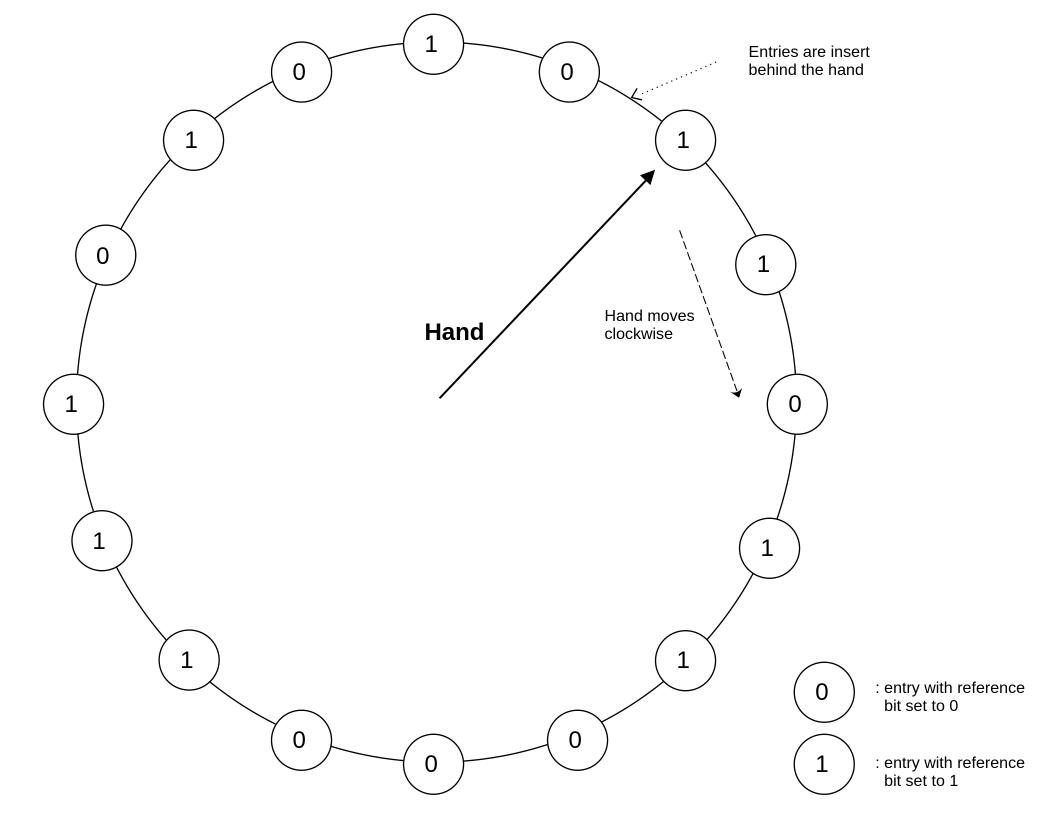
\includegraphics[scale=0.4]{clock.jpg}
	\caption{Example for circular list in CLOCK.}
		\label{fig:circular list for CLOCK}
\end{figure}

\cref{lst:clock-algorithm} shows the steps during the request of an entry.
% this doesn't sound right.
To find an entry to evict, we look at the entry to which the hand is pointing.
If the reference bit for this entry is 0, we have found the entry to be evicted.
If the reference bit is 1, we set the reference bit to 0 and move the hand to the next entry.
These steps are repeated until an entry is found whose reference bit is set to 0 and which can thus be evicted.
New insert entries are placed behind the hand which represents the tail of the list, if we see the hand as the head of the list.

\bigskip

% should try to get listing on one page, better to understand that way
\begin{lstlisting}[mathescape=true,caption=CLOCK replacement algorithm in pseudocode,label=lst:clock-algorithm]
$\textcolor{ovgu-blue}{Input}$
	Clk: Clock
	entry: entry on I/O request

if Clk.contains(entry) == true $\textcolor{ovgu-blue}{\texttt{then}}$
	// cache hit
	if entry.referenceBit == false $\textcolor{ovgu-blue}{\texttt{then}}$
		entry.referenceBit = true
	$\textcolor{ovgu-blue}{\texttt{end \ if}}$
else
	// cache miss
	if Clk.isFull() == true $\textcolor{ovgu-blue}{\texttt{then}}$
		// evict one entry
		while Clk.isFull() == true
			if Clk.hand.referenceBit == true $\textcolor{ovgu-blue}{\texttt{then}}$
				// second chance if reference bit was set
				Clk.hand.referenceBit = false
				Clk.hand = Clk.hand.next
			else
				// found entry for eviction 
				evict-candi = Clk.hand
				Clk.hand = Clk.hand.next
				Clk.evict(evict-candi)
			$\textcolor{ovgu-blue}{\texttt{end \ if}}$
		$\textcolor{ovgu-blue}{\texttt{end \ while}}$
	$\textcolor{ovgu-blue}{\texttt{end \ if}}$
	// insert entry to clock
	Clk.insert(entry)
$\textcolor{ovgu-blue}{\texttt{end \ if}}$	
return entry 
\end{lstlisting}

For our implementation in Haura, we additionally need to handle the case where the entry to be evicted is pinned and therefore cannot be cleared.
When this case occurs, we spare the entry, increment the hand, and start the search for the next entry to be eviction from there.

The advantage of CLOCK is that it does not have the problem of lock contention during cache hits, as LRU and LFU do.
This is because CLOCK does not have to maintain a priority queue and 
the update of the reference bit can be done by atomic operations. 
Therefore, no exclusive lock is required for a cache hit and 
as a result, CLOCK is more scalable than LRU and LFU in terms of 
the number of tasks accessing the cache.

Since CLOCK is an LRU approximation, it also has the same disadvantage.
The weaker performance on workloads with weak locality, like scanning and looping.

\subsection{GCLOCK}

%need to change in Haura source code
The GCLOCK replacement policy \cite{smith1978sequentiality} is a generalization of CLOCK policy.
However, the principle is already mentioned for the first time in \cite{corbato1968paging}.
Like CLOCK, GCLOCK uses a circular linked list with one hand.
But instead of only using on reference bit, a reference counter associated to each cache entry, is used.
When a cache hit occurs, the reference counter is incremented up to $K$ times.
The parameter $K$ can be chosen arbitrarily.
Also, like CLOCK, to find an entry for eviction we look at the entry the hand points to.
If the reference counter for this entry is 0, that entry is evicted.
Otherwise, we decrement the reference counter and move the pointer to the next entry 
until we find an entry with a reference counter of 0.
The \cref{lst:gclock-algorithm} shows the steps during the request of an entry.

\bigskip

\begin{lstlisting}[mathescape=true,caption=GCLOCK replacement algorithm in pseudocode,label=lst:gclock-algorithm]
$\textcolor{ovgu-blue}{Input}$
	Clk: Clock
	entry: entry on I/O request
	K: Number of max references stored per entry

if Clk.contains(entry) == true $\textcolor{ovgu-blue}{\texttt{then}}$
	// cache hit
	if entry.referenceCount < K $\textcolor{ovgu-blue}{\texttt{then}}$
		entry.referenceCount += 1
	$\textcolor{ovgu-blue}{\texttt{end \ if}}$
else
	// cache miss
	if Clk.isFull() == true $\textcolor{ovgu-blue}{\texttt{then}}$
		// evict one entry
		while Clk.isFull() == true
			if Clk.hand.referenceCount > 1 $\textcolor{ovgu-blue}{\texttt{then}}$
				// decrease reference count 
				Clk.hand.referenceCount -= 1
				Clk.hand = Clk.hand.next
			else
				// found entry for eviction 
				evict-candi = Clk.hand
				Clk.hand = Clk.hand.next
				Clk.evict(evict-candi}
			$\textcolor{ovgu-blue}{\texttt{end \ if}}$
		$\textcolor{ovgu-blue}{\texttt{end \ while}}$
	$\textcolor{ovgu-blue}{\texttt{end \ if}}$
	// insert entry to clock
	Clk.insert(entry)
$\textcolor{ovgu-blue}{\texttt{end \ if}}$
return entry 
\end{lstlisting}

When we choose $K = 0$, GCLOCK works like a FIFO policy.
For $K = 1$, GCLOCK works as an approximation to the LRU policy and is the same as the CLOCK policy.
Thus, CLOCK is a special case of the GCLOCK policy.
If we choose $K > 1$, we get an approximation to the LFU policy, but with the addition of a built-in aging mechanism.
This is because the reference counter is decremented when the hand passes an entry.
For our implementation, we use $K = 2$ because \cite{corbato1968paging} has shown that this is a good trade off between performance and additional overhead.

\subsection{CLOCK-Pro}

The CLOCK-Pro cache replacement policy \cite{jiang2005clock} combines the efficiency from CLOCK policy with the performance improvements from LIRS 
\cite{10.1145/511399.511340}.
The basic idea of CLOCK-Pro is the same as LIRS, which is to categorize cache entries into hot and cold entries based on inter-reference recency.
The hot entries always stays in cache and the cold entries allow a quick eviction of rarely accessed entries.
Also, like LIRS, CLOCK-Pro uses non-resident cold entries to track history information.
However, CLOCK-Pro, unlike LIRS, is adoptable because it does not require a predefined parameter to control the number of hot and cold entries.

To achieve better efficiency than LIRS, CLOCK-Pro combines the LRU priority queue and a FIFO queue of LIRS in a circularly linked list.
And instead of using only one hand, as in CLOCK, three hands are used to provide the functions of LIRS, 
as shown in \cref{fig:clock in clock-pro}.
For our implementation, we use a circular double linked list instead of circular single linked list, like in CLOCK.
Because in some cases me need to move a hand one entry backwards (move to predecessor) to correctly implement the motion of all hands.
Since the hands should not point to the same entry.

\begin{figure}[ht]
	\centering
	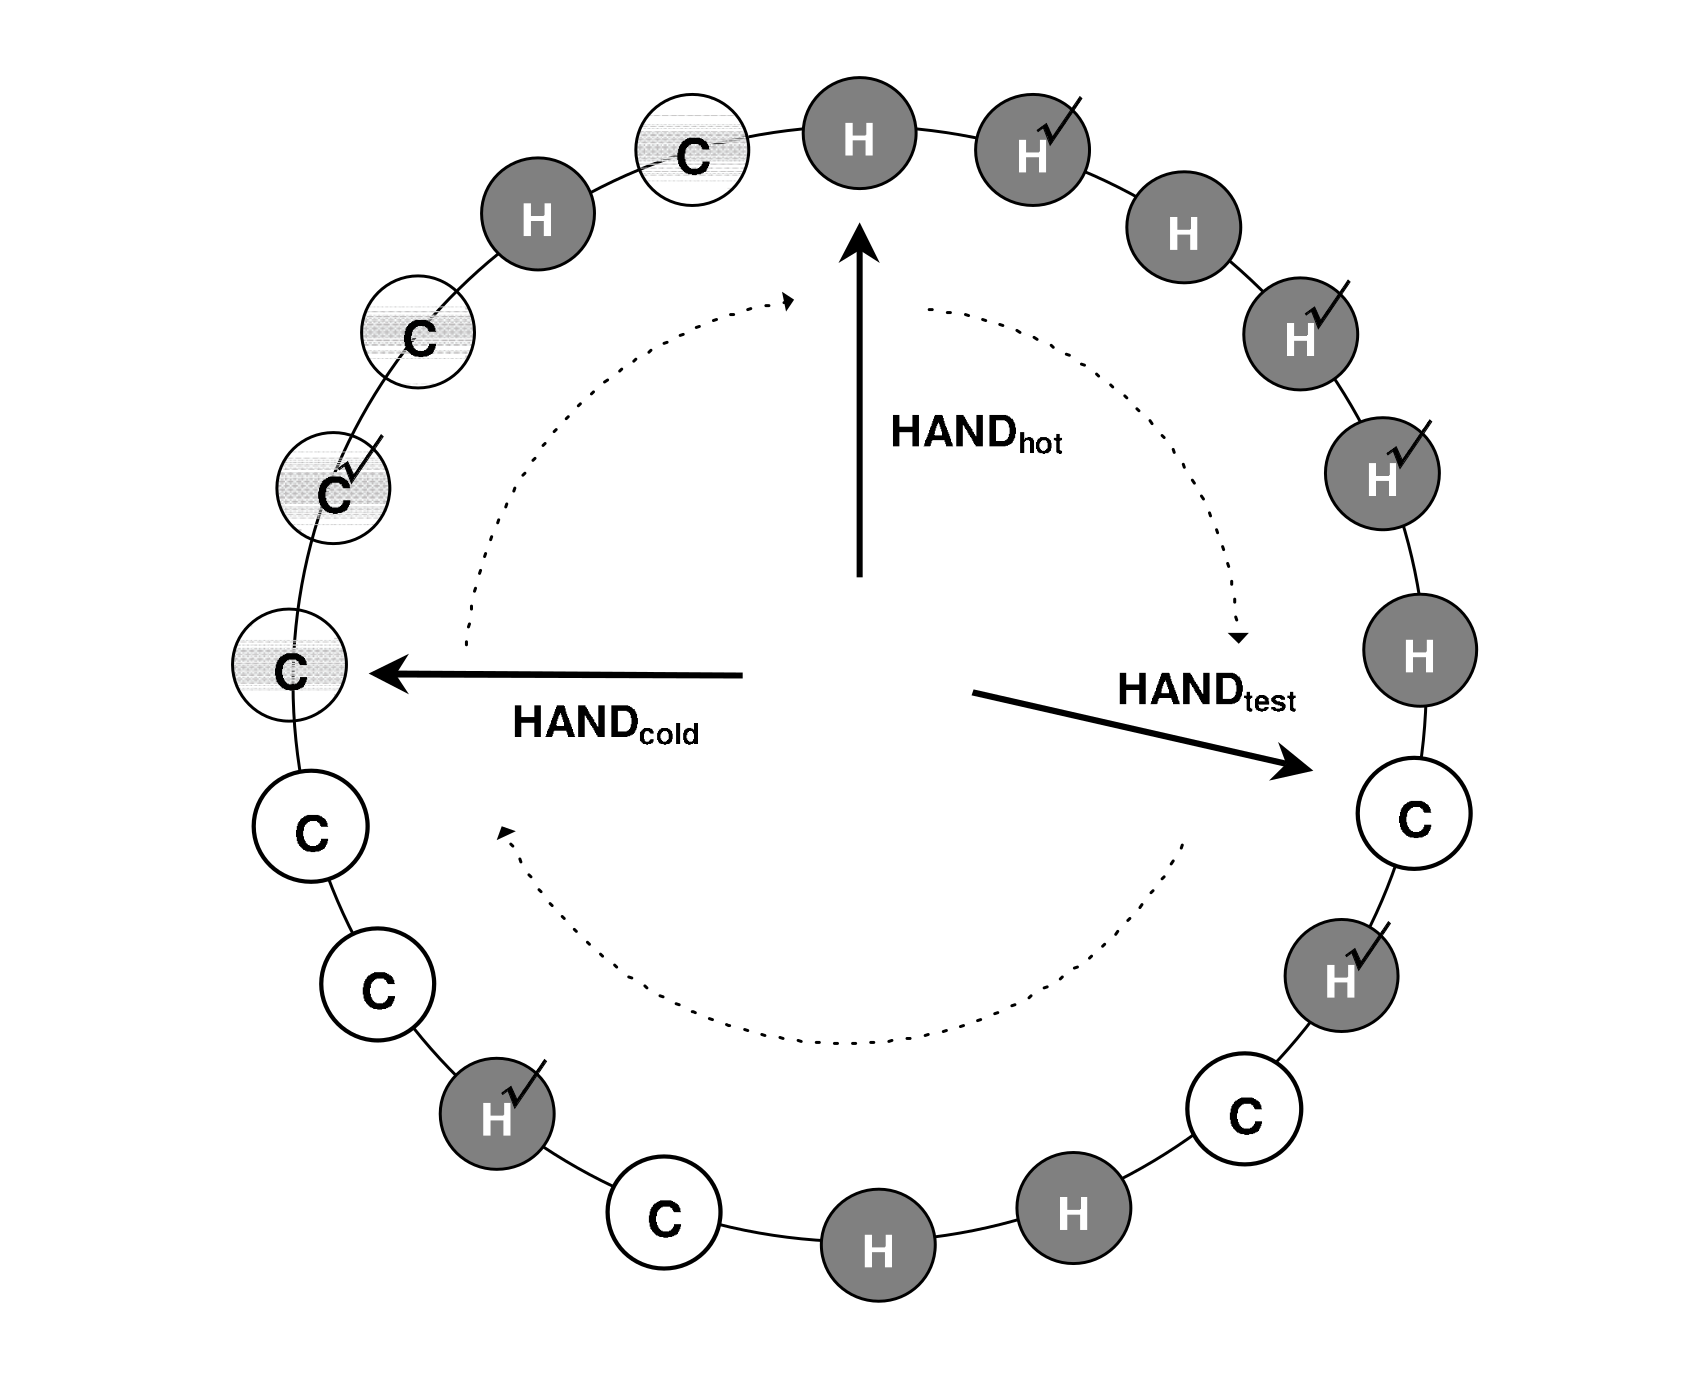
\includegraphics[scale=0.2]{clock_pro.png}
	\caption{Example of the circular list for CLOCK-Pro. Hot entries marked with "H", cold entries with "C" and non-resident cold entries are shadowed.
	The "$\sqrt{}$" marks referenced entries.}
		\label{fig:clock in clock-pro}
\end{figure}

For each entry we need to store additional metadata. This includes whether it is a hot or cold entry, is it resident or non-resident in the cache, has it been referenced in the near past, and is the entry in the test phase.
Each Hot Entry is always resident and not in the testing phase.
Cold entries, on the other hand, may be resident or non-resident and may or may not be in the testing phase.
Also, all newly inserted entries are resident cold entries in the test phase.
Both can be referenced or not.
The test phase is used to give cold entries the chance to turn into hot entries.
As we will see in a moment.

The $\textbf{Hand}_{hot}$ marks the tail of the list and therefore points to the last hot entry.
Also, $\textbf{hand}_{hot}$ turns unreferenced hot entries into cold entries  and removes the reference for referenced hot entries when it passes over them.


The $\textbf{Hand}_{cold}$ is used to find the entry for eviction. 
In this respect $\textbf{Hand}_{cold}$ operates like the hand in CLOCK.
This means that $\textbf{hand}_{cold}$ will traverse all entries until it finds a resident cold entry that is not referenced and thus can be evicted.
If the entry to be evicted is in the test phase, it remains in the cache as a non-resident entry, if it is not in the test phase, it is completely evicted from the cache.
So if there are only hot entries in the cache,  
we must first convert hot entries to cold entries in order to evict an entry.
Furthermore, $\textbf{Hand}_{cold}$ turn referenced cold entries in test phase to hot entries. 
This is because the reference during test phase means that the inter-reference recency for this entry is low enough to be a categorized as an hot entry.

And the $\textbf{Hand}_{cold}$ marks the last entry in test phase and ends the test phase for all resident cold entries when it moves over them. 
It also evicts passed non-resident cold entries from the cache.
The reason for this is that non-resident cold entries that have not already been converted to hot entries have a high inter-reference recency 
and therefore should not become hot entries.

The \cref{lst:clock-pro-algorithm} shows the steps during the request of an entry.
What we see is that all hands work together to find an entry for eviction, \cref{lst:clock-pro-algorithm} line 12 to line 65.

\bigskip
% better to use newpage in final version to avoid that the listing spans over 3 pages
%\newpage

\begin{lstlisting}[mathescape=true,caption=CLOCK-Pro replacement algorithm in pseudocode,label=lst:clock-pro-algorithm]
$\textcolor{ovgu-blue}{Input}$
	Clk: Clock
	entry: entry on I/O request

if Clk.contains(entry) == true $\textcolor{ovgu-blue}{\texttt{then}}$
	// cache hit
	if entry.referenceBit == false $\textcolor{ovgu-blue}{\texttt{then}}$
		entry.referenceBit = true
	$\textcolor{ovgu-blue}{\texttt{end \ if}}$
else
	// cache miss
	if Clk.isFull() == true $\textcolor{ovgu-blue}{\texttt{then}}$
		while Clk.countHot + Clk.countCold >= Clk.capacity
			// run cold-hand to find evict candidate
			evict-candi = Clk.coldHand
			if evict-candi.coldBit == true $\textcolor{ovgu-blue}{\texttt{then}}$
				if evict-candi.referenceBit == true $\textcolor{ovgu-blue}{\texttt{then}}$
					// turn evict-candi to hot entry
					evict-candi.hotBit == true
					evict-candi.coldBit == false
					Clk.countHot += 1
					Clk.countCold -= 1
				else
					// turn resident Cold entry to non-resident Cold entry
					// only retain key and metadata
					Clk.turnNonResident(evict-candi)
					Clk.countCold -= 1
					Clk.countTest += 1	
				$\textcolor{ovgu-blue}{\texttt{end \ if}}$
			$\textcolor{ovgu-blue}{end \ if}$
			// move test hand if necessary
			while Clk.countTest > Clk.testCapacity
				// test hand turns resident cold entry to non-resident cold entry
				// if still in test-period
				entry = Clk.testHand
				if entry.testBit == true $\textcolor{ovgu-blue}{\texttt{then}}$
					Clk.testHand = Clk.testHand.next
					Clk.removeNonResidentEntry(entry)
					Clk.countTest -= 1
					if Clk.coldCapacity > 1
						Clk.coldCapacity -= 1
					$\textcolor{ovgu-blue}{\texttt{end \ if}}$
				$\textcolor{ovgu-blue}{\texttt{end \ if}}$
				Clk.testHand = Clk.testHand.next
			$\textcolor{ovgu-blue}{\texttt{end \ while}}$
			// move cold hand
			Clk.coldHand = Clk.coldHand.next
			// move hot hand if necessary
			while Clk.countHot > Clk.capacity - Clk.coldCapacity
				// hot hand removes reference bit on hot entry 
				// or turn not referenced hot entry to cold entry
				entry = Clk.hotHand
				if entry.hotBit == true $\textcolor{ovgu-blue}{\texttt{then}}$
					if entry.referenceBit == true $\textcolor{ovgu-blue}{\texttt{then}}$
						entry.referenceBit == false
					else
						entry.hotBit = false
						entry.coldBit = true
						Clk.countHot -= 1
						Clk.countCold += 1
					$\textcolor{ovgu-blue}{\texttt{end \ if}}$
				$\textcolor{ovgu-blue}{\texttt{end \ if}}$
				Clk.hotHand = Clk.hotHand.next
			$\textcolor{ovgu-blue}{\texttt{end \ while}}$
		$\textcolor{ovgu-blue}{\texttt{end \ while}}$
	Clk.insert(entry)
$\textcolor{ovgu-blue}{\texttt{end \ if}}$	
return entry 
\end{lstlisting}

For a cache with capacity $m$ applies $m = m_c + m_h$.
Here $m_c$ is the capacity for resident cold entries and $m_h$ is the capacity for hot entries.
Furthermore, at most $m$ non-resident cold entries can be stored.
So that the cache actual size can be at most $2m$ entries.
To achieve adaptability, the number of hot and cold entries is not fixed.
The capacity for resident cold entries $m_c$ is increased by one, if an cold entry is accessed during its test phase 
and $m_c$ is decreased by one, if a cold entry leaves its test phase without being re-accessed.
As we see in \cref{lst:clock-pro-algorithm} the actual hand movements are triggered by the count of hot and cold entries and the 
capacity for hot and cold entries.
This changes the behavior of CLOCK-Pro depending on the underlying workload.

When $m_c$ is large, CLOCK-Pro behaves similarly to LRU. But if $m_c$ is small it behaves like LIRS.
The small $m_C$ leads to a quicker eviction of newly inserted entries and the entries with low inter-reference recency, hot entries, have a higher 
chance to stay in cache. Thus, in theory, CLOCK-Pro has the advantage of LRU for workloads with strong locality and 
the advantages of LIRS for workloads with weak locality.

In our implementation in Haura, we have to modify the CLOCK-Pro, due to the fact that the DMU manages the cache.
So we can not turn non-resident cold entries to hot entries, which are always resident.
Because this would imply that the cache tells the DMU what to do and not the other way around.

Furthermore, the treatment of a pinned entry during eviction, is more complicated then for CLOCK and GCLOCK.
We have already seen that for eviction all pointers work together. If the entry intended for eviction remains in the cache, it can happen that a 
hand gets stuck on this entry, since the entry is pinned it cannot be removed. This can lead to an endless loop. To prevent this, this entry is 
removed and temporally saved. So that the hands can work as intended.
If it then occurs that the entry is pinned, the entry is again insert into the cache.

\subsection{ML-CLOCK}
\label{sub:ml-clock}

The last cache replacement policy implemented is ML-CLOCK by \cite{cho2021ml} and 
follows the recent trend of incorporating machine learning techniques.
The idea for ML-CLOCK is to use recency and frequency information for eviction.
In order to achieve adaptability, we cannot use a fixed weighting parameter as we have seen with LRFU \cite{lee2001lrfu}. 
If the weighting parameter is fixed, we cannot adapt to the access pattern.
So instead of using a fixed parameter to decide what is more important, recency 
or frequency,
ML-CLOCK learns the weighting parameter from previous decisions and is therefore adaptive.

In addition, ML-CLOCK is designed to minimize writes to the underlying storage devices.
The motivation for this is that write operations take more time than read operations.
Also, some memory types like flash memory, can only write in blocks.
Thus we can minimize write operations, if we manage to write back adjacent data blocks, 
instead of writing back data scattered across a storage device.

For each entry we have a reference bit, a reference counter and a time stamp of the 
last accesses as metadata. 
Also the entries are categorized in clean (unmodified) entries and dirty (modified) entries.
And in contrast to the other implemented cache replacement policies,
ML-CLOCK uses two circular linked lists.
One for the clean entries which we refer to as clean-clock 
and a second for the dirty entries which we will refer to as dirty-clock
which is also sorted by the logical block address for each entry.
Both circular list have one hand, the c-hand for the clean-clock and 
the d-hand for the dirty-clock.
When the d-hand move to the next entry, it moves the next entry 
which has the closest address in the dirty clock.
This ensures that sequential blocks are written back, if possible.
Furthermore, we use a ghost queue which saves the metadata of evicted entries and 
is used to train the SLP.
At most the ghost queue can store as many entries as the cache, clean-clock and dirty-clock together.

ML-CLOCK uses a single-layer perceptron(SLP).
SLP is a binary classifier, which in our case predicts whether an entry should be evicted or not.
One advantage of SLP compared to more advanced machine learning techniques, such 
as multi-layer perceptrons or long short-term memory networks, is that
SLP has low time and space overhead,
making it more suitable for online learning.
Furthermore, SLP are not prone to overfitting.

To predict if an entry will be evicted the following equation \ref{prediction} is used,\\
where $w_d, w_c$ and $w_b$ represents the weight for reuse-distance, reference count and the bias.
The variables $x_d$ and $x_c$ represents the metadata values from the entry reuse-distance and the reference count.

\begin{align}
	f_{predict} (x_d, x_c) =
	\begin{cases}
		0, \quad x_d \cdot w_d + x_c \cdot w_c + 1 \cdot w_b < 0 \\
		1, \quad x_d \cdot w_d + x_c \cdot w_c + 1 \cdot w_b \geq 0 \label{prediction}
	\end{cases}
\end{align}

Also, $x_d$ must be scaled down so that it has the same order of magnitude as $x_c$, as shown in equation \ref{reduction}.

\begin{align}
	x_d = \frac{\emph{current timestamp} - \emph{timestamp of the last access}}{\emph{number of all entries in cache}} \label{reduction}
\end{align}
	
In addition to learning the weights $w_d, w_c$ and $w_b$, the equation \ref{learning} is used.

\begin{align}
\begin{split}
	w_d \leftarrow w_d + lr \cdot x_d \cdot (v_{expect} - v_{predict})\\
	w_c \leftarrow w_c + lr \cdot x_c \cdot (v_{expect} - v_{predict})\\
	w_b \leftarrow w_b + lr \cdot x_b \cdot (v_{expect} - v_{predict})\\
\end{split} \label{learning}
\end{align}

The learning rate $lr$ controls how much the weights changes during training.
The variable $v_{predict}$ is the result of an prediction, equation \ref{prediction}, for an entry and 
$v_{expect}$ is the correct answer for this prediction, as we see in listing \ref{lst:clock-algorithm}.
Both $v_{predict}$ and $v_{expect}$ can either be 1 or 0.
Thus, the term $(v_{expect} - v_{predict})$ defines if the weights are updated or not.


\cref{lst:clock-algorithm} shows the steps during the request of an entry and also shows when 
the prediction and the learning take place.

\bigskip

\begin{lstlisting}[mathescape=true,caption={ML-CLOCK replacement algorithm in pseudocode, slightly modified from \cite{jiang2005clock}},label=lst:ml-clock-algorithm]
$\textcolor{ovgu-blue}{Input}$
	Clk: Clock
	hand: hand is the entry the clock hand is pointing to
	entry: entry on I/O request
	GhostQ: Ghost Queue

if Clk.contains(entry) == true $\textcolor{ovgu-blue}{then}$
	updateMetadata(entry)
	// trigger learning operation
	// second parameter for learning() is $\textcolor{gray}{v_{expect}}$
	learning(entry, 1)
	return entry
else
	// cache miss
	if Clk.isFull() == true $\textcolor{ovgu-blue}{then}$
		// scan clean pages at the C-hand's location
		C-candi = Clk.findCleanCandidate()
		// scan dirty pages at the D-hand's location
		// in a sequential order (i.e, LBA)
		D-Candi = Clk.findDirtyCandidate()
		victim = prediction(C-candi, D-candi)
		// check if victim is in ghost queue
		if GhostQ.findPage(victim) == true $\textcolor{ovgu-blue}{then}$
			// ready to promote a entry to clock
			// second parameter for learning() is $\textcolor{gray}{v_{expect}}$
			learning(entry, 1)
			GhostQ.deleteEntry(victim)
		else
			if GhostQ.isFull() == true $\textcolor{ovgu-blue}{then}$
				// evict a page on ghost queue with learning
				// second parameter for learning() is $\textcolor{gray}{v_{expect}}$
				learning(GhostQ.tail, 0)
				GhostQ.deleteEntry(GhostQ.tail)
			$\textcolor{ovgu-blue}{end \ if}$
			GhostQ.insertEntry(victim)
		$\textcolor{ovgu-blue}{end \ if}$
		Clk.evict(victim)
	$\textcolor{ovgu-blue}{end \ if}$
	// insert entry to clock
	Clk.insert(entry)
$\textcolor{ovgu-blue}{end \ if}$
return entry 
\end{lstlisting}

On a cache hit, we update the metadata for the entry and start a learning operation.
We set $v_{expect}$ to 1, because the requested entry is contained in cache.
Then we use the metadata of the entry to make a prediction, equation \ref{prediction}, and get $v_{predict}$.
The weights are updated or not based on $v_{expect}$ and $v_{predict}$.
In addition, a cache hit may cause a clean entry to become a dirty entry.
Therefore, the entry is moved from the clean-clock to the dirty-clock.
For this case, we added the \texttt{get\_mut}()-function to the Cache trait.
% could be insert chapter for cache trait.

To find a entry for eviction during a cache miss, 
we search for eviction candidates in both clocks.
Like the hand in CLOCK, the c-hand and d-hand search for an entry with the reference bit set to 0.
So there are two eviction candidates, the c-candidate from the clean-clock and the d-candidate from the dirty-clock.
The next step is to apply the prediction operation to both candidates and to decide which candidate to evict the preference 
rules in \cref{tab:ml-clock preference rules} will be used.
Since the goal is to minimize write operations, in 3 out of 4 possible cases the c-candidate is removed and not the d-candidate.

\begin{table}[ht]
	\centering
	\begin{tabular}{|c|c|c|}
		\hline
		\textbf{Predicted Value} & \textbf{Predicted Value} & \textbf{Victim Entry} \\
		\textbf{(c-candidate)} & \textbf{(d-candidate)} & \\
		\hline
		0 & 0 & C-Candidate \\
		\hline
		0 & 1 & C-Candidate \\
		\hline
		1 & 0 & D-Candidate \\
		\hline
		1 & 1 & C-Candidate \\
		\hline
	\end{tabular}
	\caption{Preference rules for victim entry \cite{cho2021ml}}
	\label{tab:ml-clock preference rules}
\end{table}


When the entry to evict was found,
it is checked whether this entry is already in the ghost queue.
If this is the case, a learning operation is triggered.
Additionally, the entry is evicted from the Ghost queue and added back to the cache.
In our implementation, we do not reinsert the entry into the cache for the same reason as in CLOCK-Pro, the DMU
manages which entries are inserted into the cache and not the cache itself.

In case the entry for eviction is not already in the ghost queue, it will be insert into the ghost queue.
An learning operation is triggered if the ghost queue exceeds it capacity and thus an ghost entry at the front leaves the ghost queue.

So there are three possibilities to trigger a learning operation during a cache hit, 
if the entry for eviction is already in the ghost queue or
if a entry must leave the ghost queue.

The case that the entry for eviction is pinned can be handled the same way as in CLOCK and GCLOCK, 
simple leave the pinned entry in the clock and continue the search at the next entry.


\section{Summary}

The basis for the data management in Haura is the DML state cycle.
Each object can be in one of the four states on disk, unmodified, modified or in write back.
Also the DML specifies which state changes are possible.
In particular, the fact that objects cannot leave or enter the cache when in modified or 
write back state, the pinned entries, requires significant adjustments to the cache policy.

The implemented cache replacement policies followed the improvement strategies from the \cref{sec:improved cache replacement policies}.
The first implemented policy was CLOCK, which was already implemented.
CLOCK is an LRU approximation which uses a circular linked list, instead of an priority queue as LRU does.
By using a circularly linked list, CLOCK achieves similar performance to LRU with lower overhead.

The next policy was GCLOCK, which is generalization of CLOCK, and uses a reference counter instead of only a reference bit.
Thus, GCLOCK can use more history information for the eviction decision.

The CLOCK-Pro replacement policy uses the inter-reference recency, a measure for the reuse distance, to separate entries into
hot (low reuse distance) and cold (high reuse distance) entries.
The hot entries have a high chance to be reused again in near future and should therefore stay in cache and
the cold entries with low chance to be reused again in near future should be evicted first.

CLOCK-Pro is an example of a cache replacement policy that recognizes access patterns.
It uses the inter-reference recency to distinguish between hot and cold entries and handle these entries differently.
The last implemented cache replacement policy, ML-CLOCK, is an example for an policy that uses machine learning.
A model is trained based on the removed entries and the cache hits. 
This model is then used to find the entry for the eviction.

The last implemented policy was ML-CLOCK, which uses a single-layer perceptron to learn from the evicted entries and 
from the cache hits whether an entry should be evicted or not.
In contrast to more advanced machine learning algorithm, a single-layer perceptron is easy to implement, no additional libraries are required 
and has a low runtime overhead.
Also, unlike the other cache replacement policies, ML-CLOCK attempts not only to minimize cache misses,
but also to minimize writes to the underlying storage medium.
For this reason, ML-CLOCK uses two circular linked list, one for the clean (not modified) 
and one for the dirty (modified) entries.

\chapter{Evaluation}
\label{cha:evaluation}

% detalierte Beschreibung des Testsystems und der Testumgebung, Software Hardware etc.
% soll reproduzierbar sein
% Wie soll man die Daten angeben reicht Diagramme?
% was sind die Kriterien für die Evaluation, Latenz, Cache-misses, Ausführungszeit, ...
% Interpretation der Resultate
% Vorteile und Nachteile darstellen

% 25-35%, ca. 10-14 Seiten

In this chapter, we evaluate the implemented cache replacement policies which we described in \cref{cha:design and implementation}.
First, we will describe the used hardware and software for the performance evaluation.
After that, we explain how the benchmarks for performance evaluation are constructed and why we chose them.
And lastly, we look at the results of the evaluation which we divided in singled threaded and multi-threaded workloads.

\section{Setup}

%- centos stream 8
%- kernel 4.18.0-512.el8.x86_64
%- AMD Epyc 7443 2.85 GHz 24 cores
%- 128 GB RAM
%- storage on CephFS
%- haura config could be in appendix 


For the evaluation the HPC-cluster of the Otto-von-Guericke-University was used.
The HPC cluster of the Otto-von-Guericke-University was used for the evaluation.
The \cref{tab:hardware node} shows the hardware of the used node.
As secondary storage, we used the home folder which is shared between all nodes and uses CephFS.

\begin{table}[ht]
	\centering
	\begin{tabular}{|c|c|}
		\hline
		\textbf{CPU} & AMD Epyc 7443\\
		\hline
		\textbf{cores per CPU} & 24\\
		\hline
		\textbf{base clock CPU} & 2.85\\
		\hline
		\textbf{RAM} & 128 GB DDR4\\
		\hline
		\textbf{Secondary storage} & shared CephFS across all nodes \\
		\hline
	\end{tabular}
	\caption{Hardware for evaluation}
	\label{tab:hardware node}
\end{table}

-> next used software

\section{Methodology}

%%- used 1GiB cache which is relatively small to actually see cache misses
%%- conisderble larger cache would need much larger I/O files to actually show misses
%- synthetic benchmarks with fio zipf and random, if I get random to work\\
%- zip benchmark with linux kernel source files\\
%% \cite{karakostas2000practical} -> contains zipfian distribution as use case for webcaches
%- only synthetic benchmarks 
%- zipf, normal, zoned, uniform 


\section{Single threaded}

\begin{figure}[H]
	\centering
	\begin{subfigure}{0.4\textwidth}
		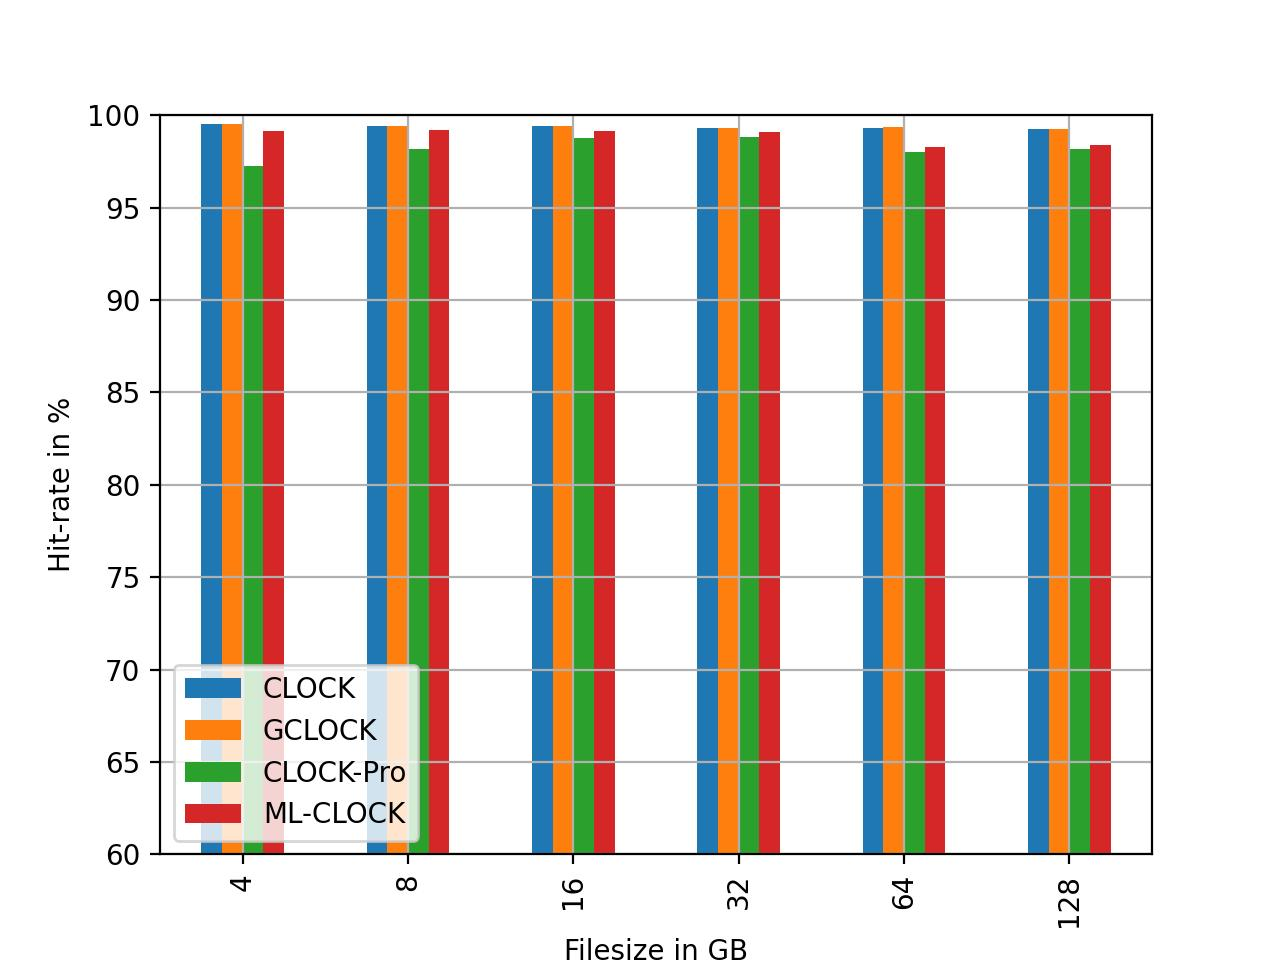
\includegraphics[width=\textwidth]{randread_zipf.jpg}		
		\caption{Zipf-distribution}
		\label{fig:randread zipf}
	\end{subfigure}
	\hfill
	\begin{subfigure}{0.4\textwidth}
		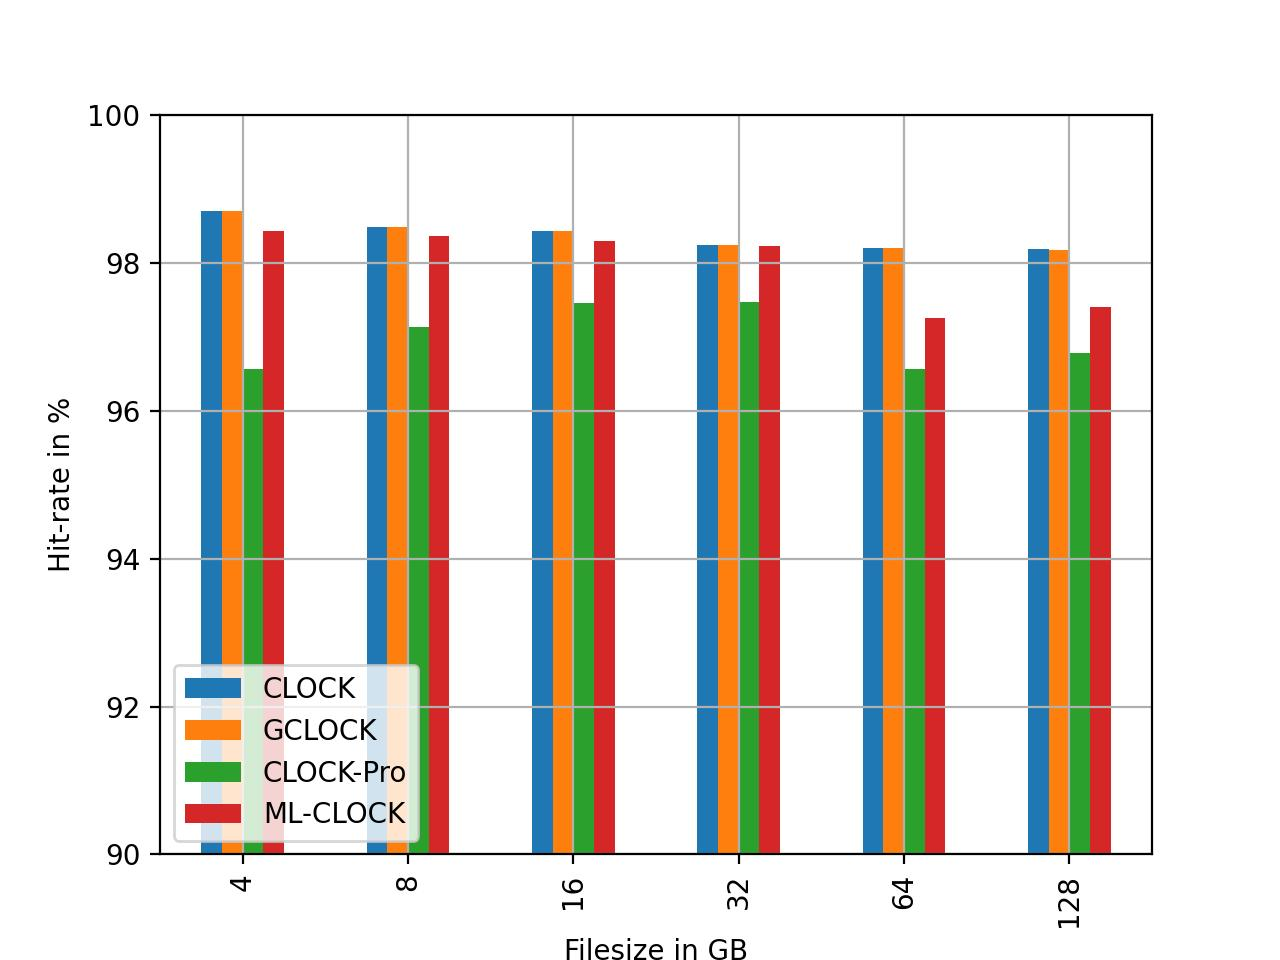
\includegraphics[width=\textwidth]{randread_normal.jpg}		
		\caption{Normal-distribution}
		\label{fig:randread normal}
	\end{subfigure}
	\hfill
	\begin{subfigure}{0.4\textwidth}
		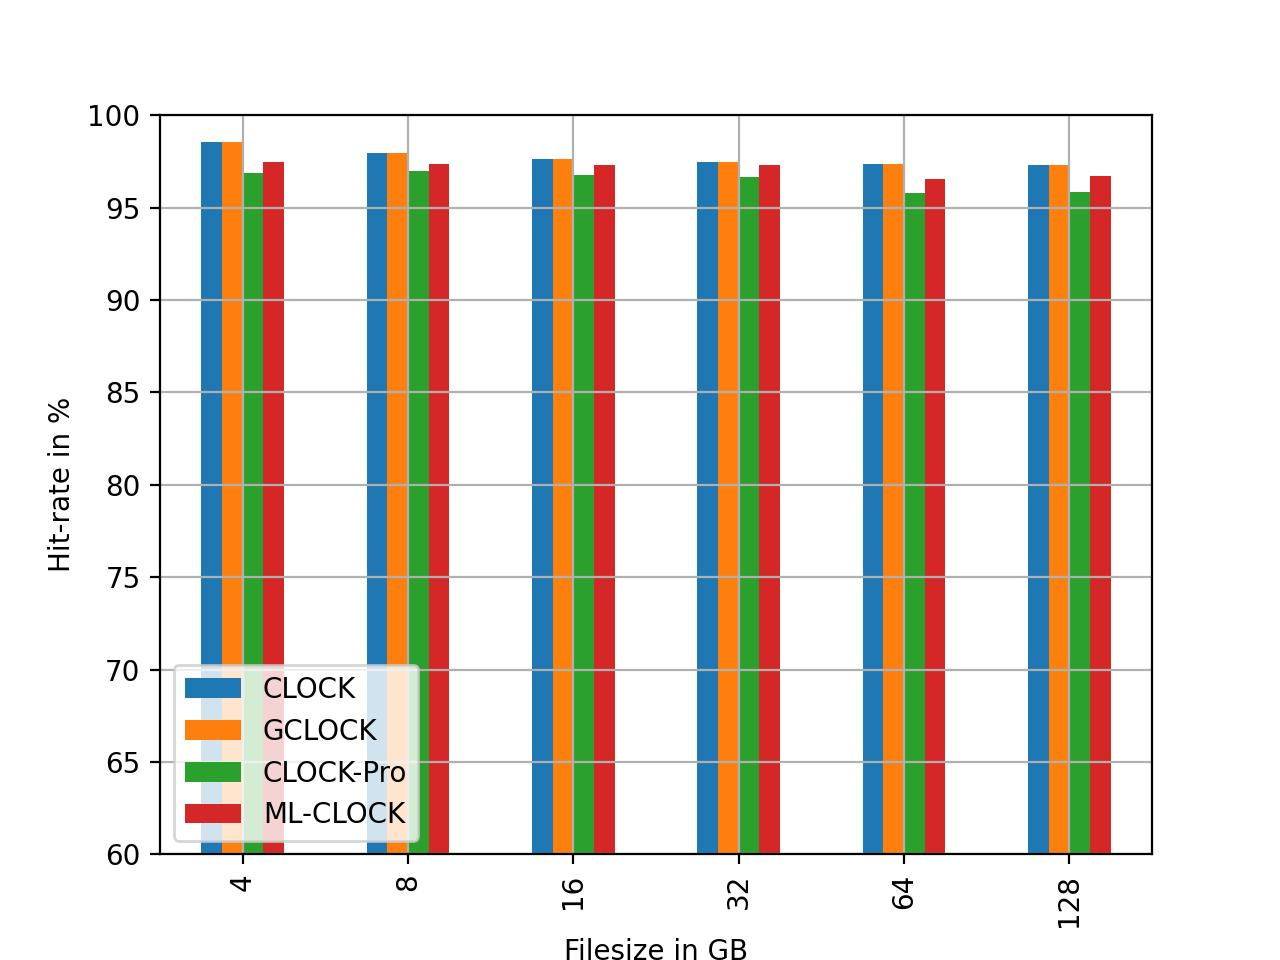
\includegraphics[width=\textwidth]{randread_zoned.jpg}		
		\caption{Zoned-distribution}
		\label{fig:randread zoned}
	\end{subfigure}
	\hfill
	\begin{subfigure}{0.4\textwidth}
		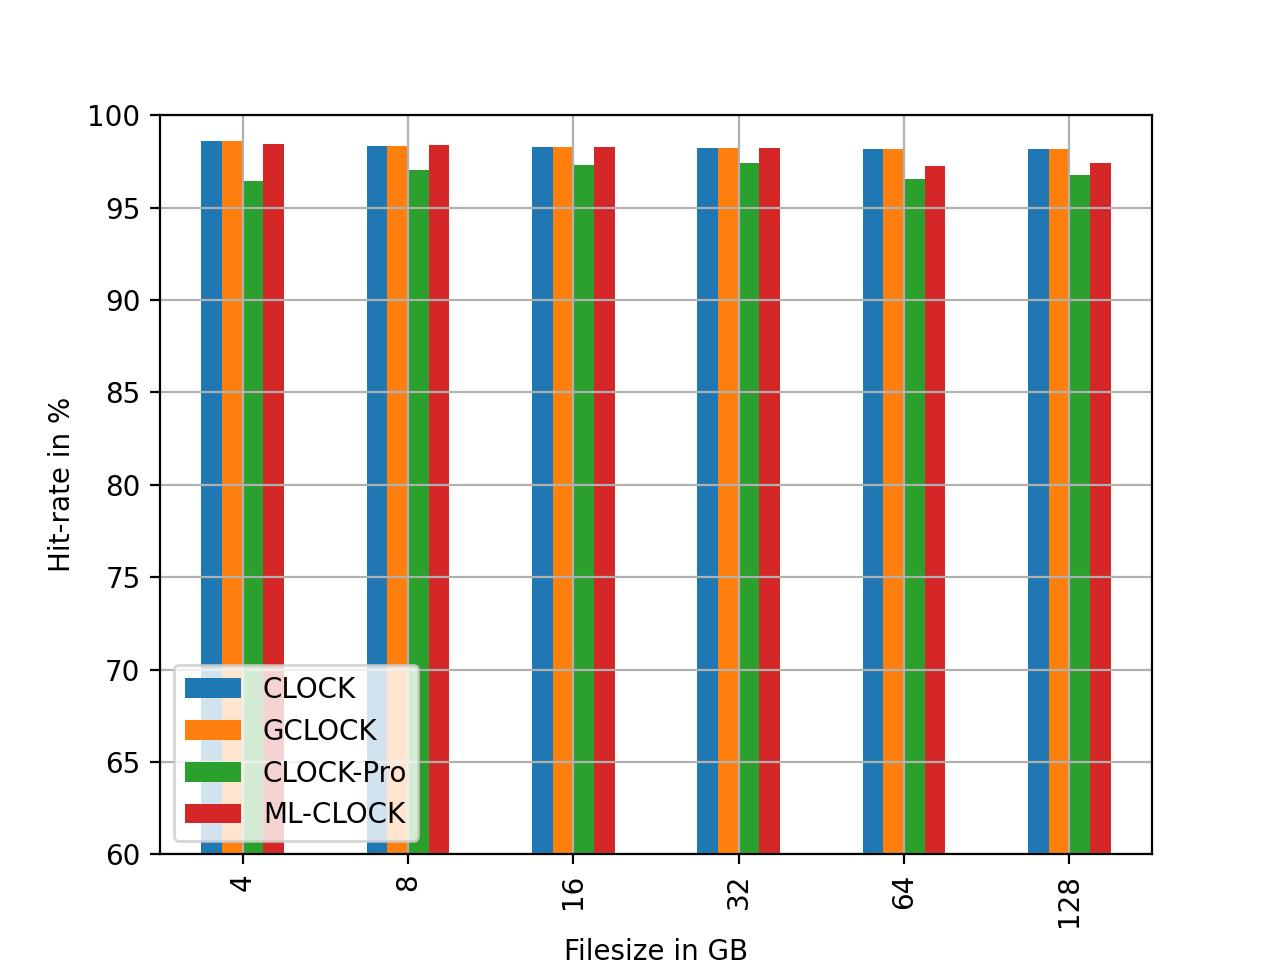
\includegraphics[width=\textwidth]{randread_uniform.jpg}		
		\caption{Uniform-distribution}
		\label{fig:randread uniform}
	\end{subfigure}
	\caption{These figures show the hit-rate file-size diagram for each implemented cache replacement policy for random read-only workload with different 				random distributions.}
\end{figure}

%-------------------------------------------------------

\begin{figure}[H]
	\centering
	\begin{subfigure}{0.4\textwidth}
		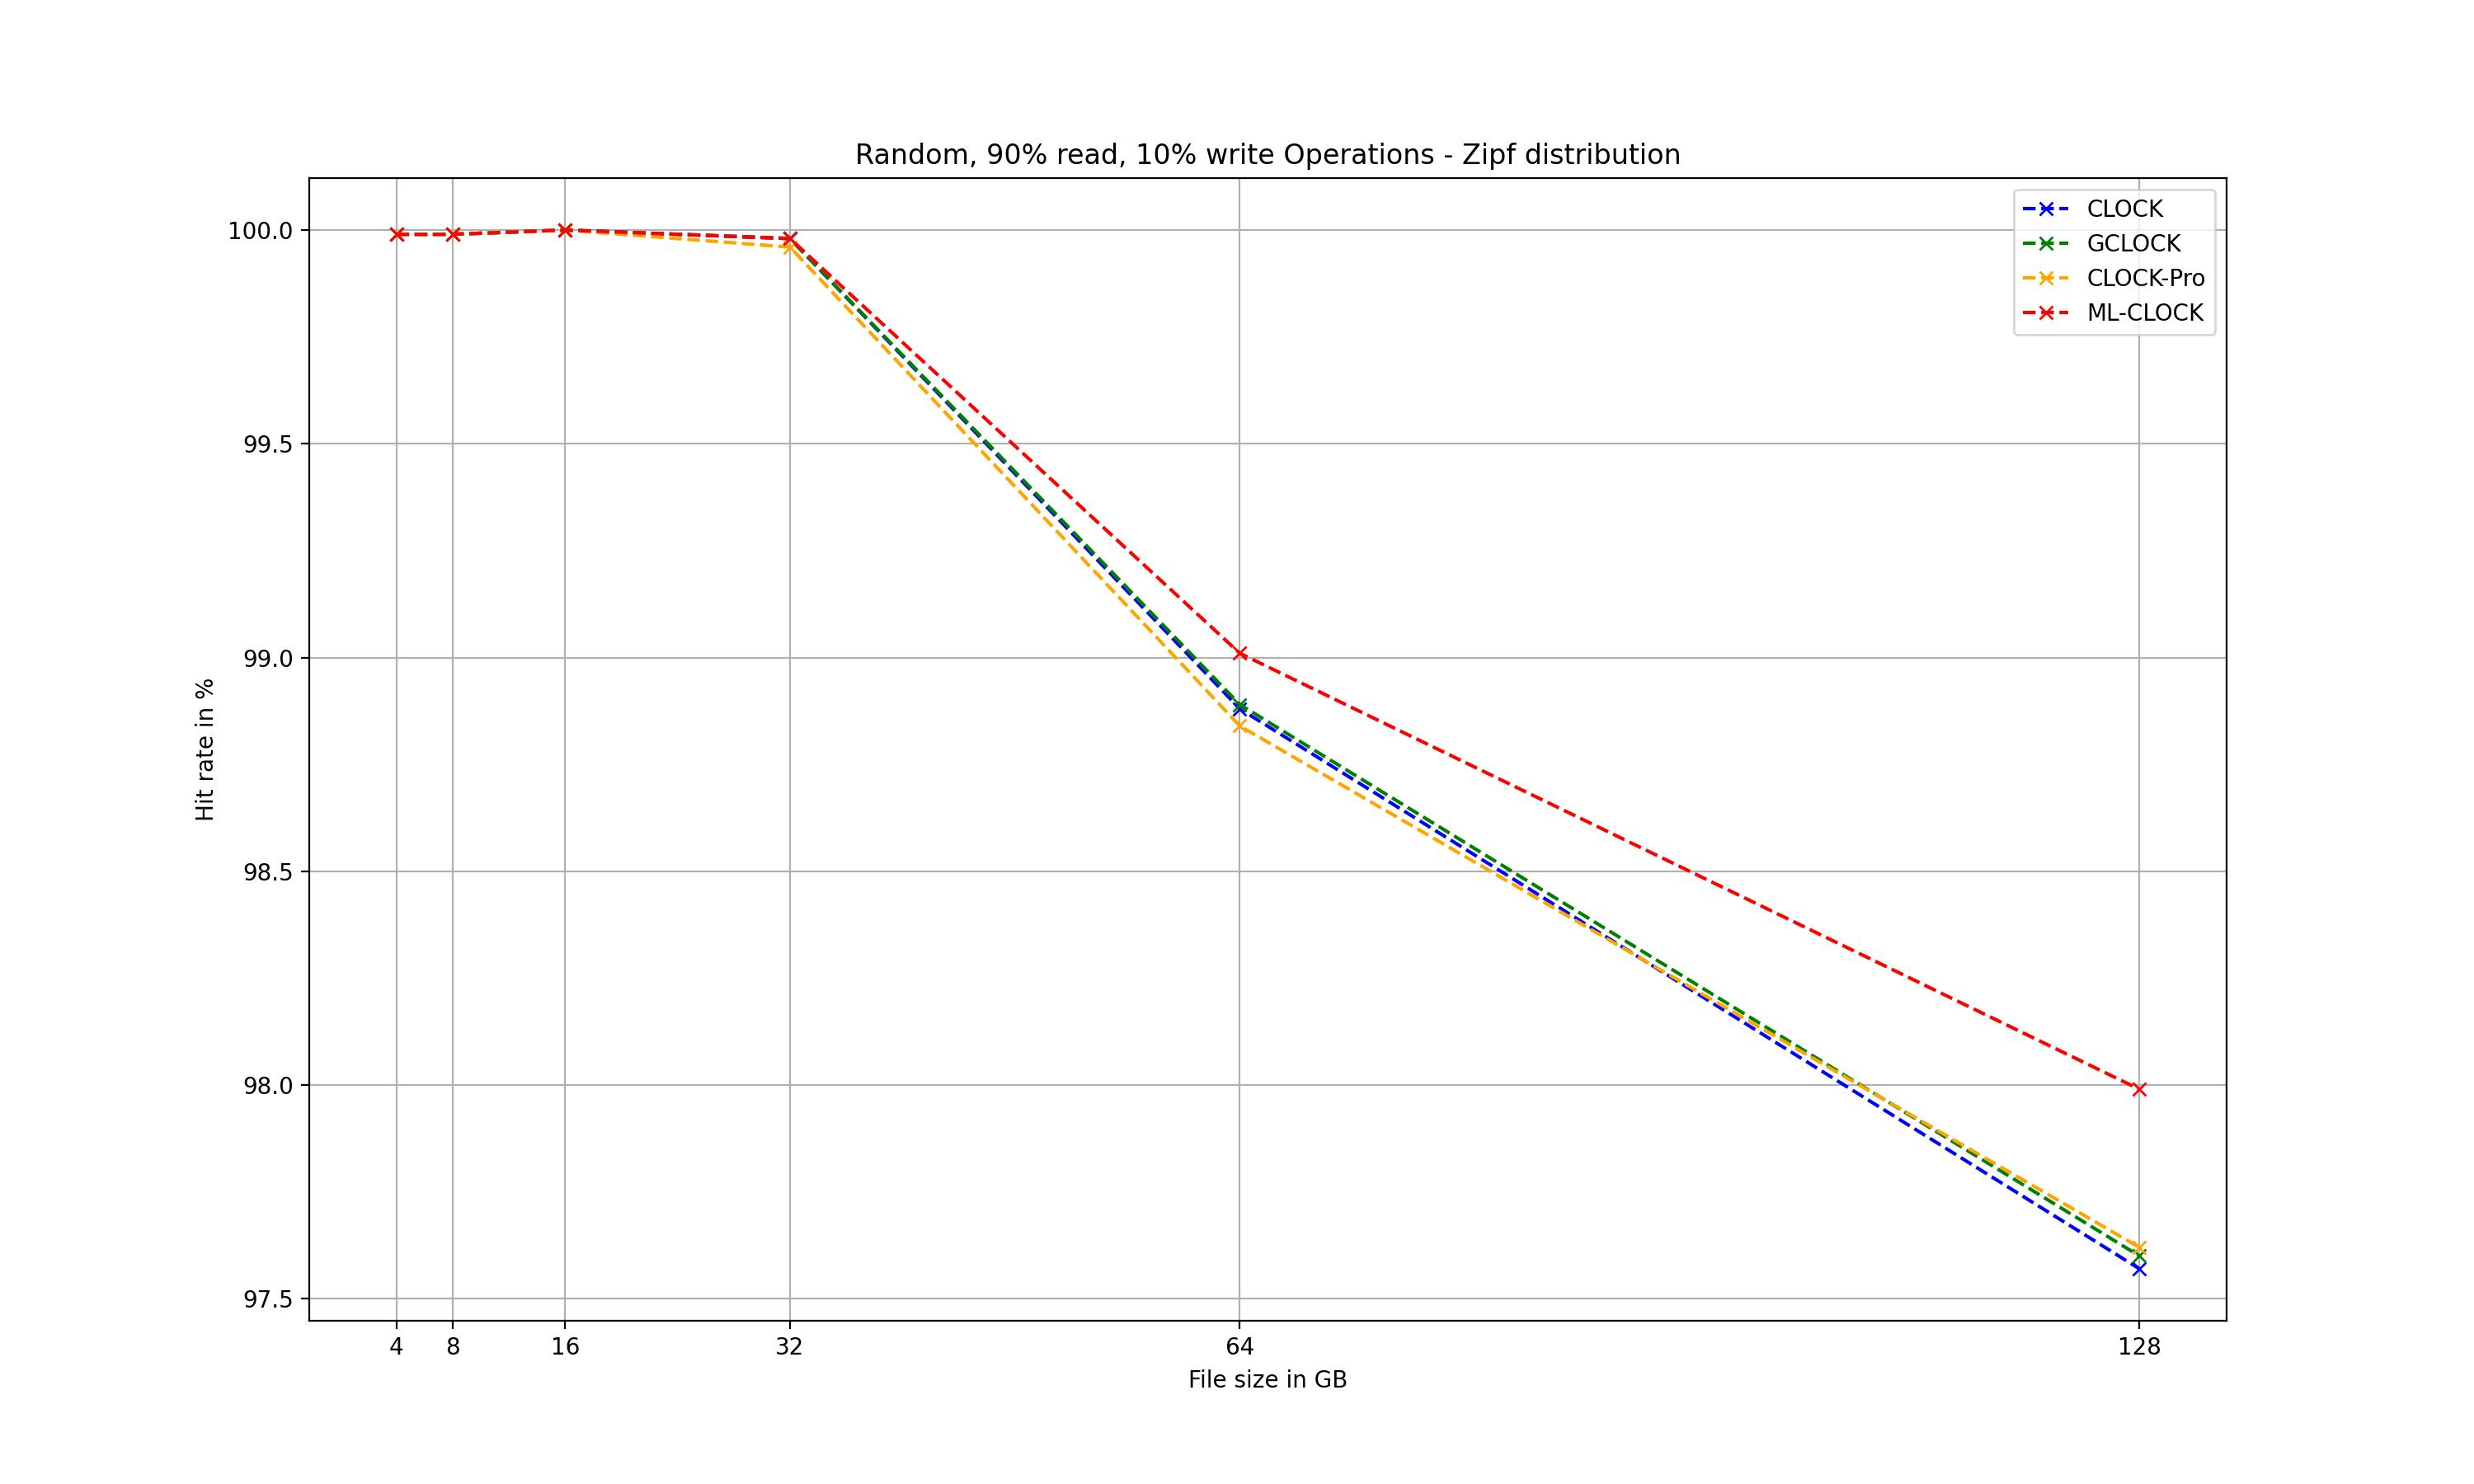
\includegraphics[width=\textwidth]{rw_90to10_zipf.jpg}		
		\caption{Zipf-distribution}
		\label{fig:rw_90to10  zipf}
	\end{subfigure}
	\hfill
	\begin{subfigure}{0.4\textwidth}
		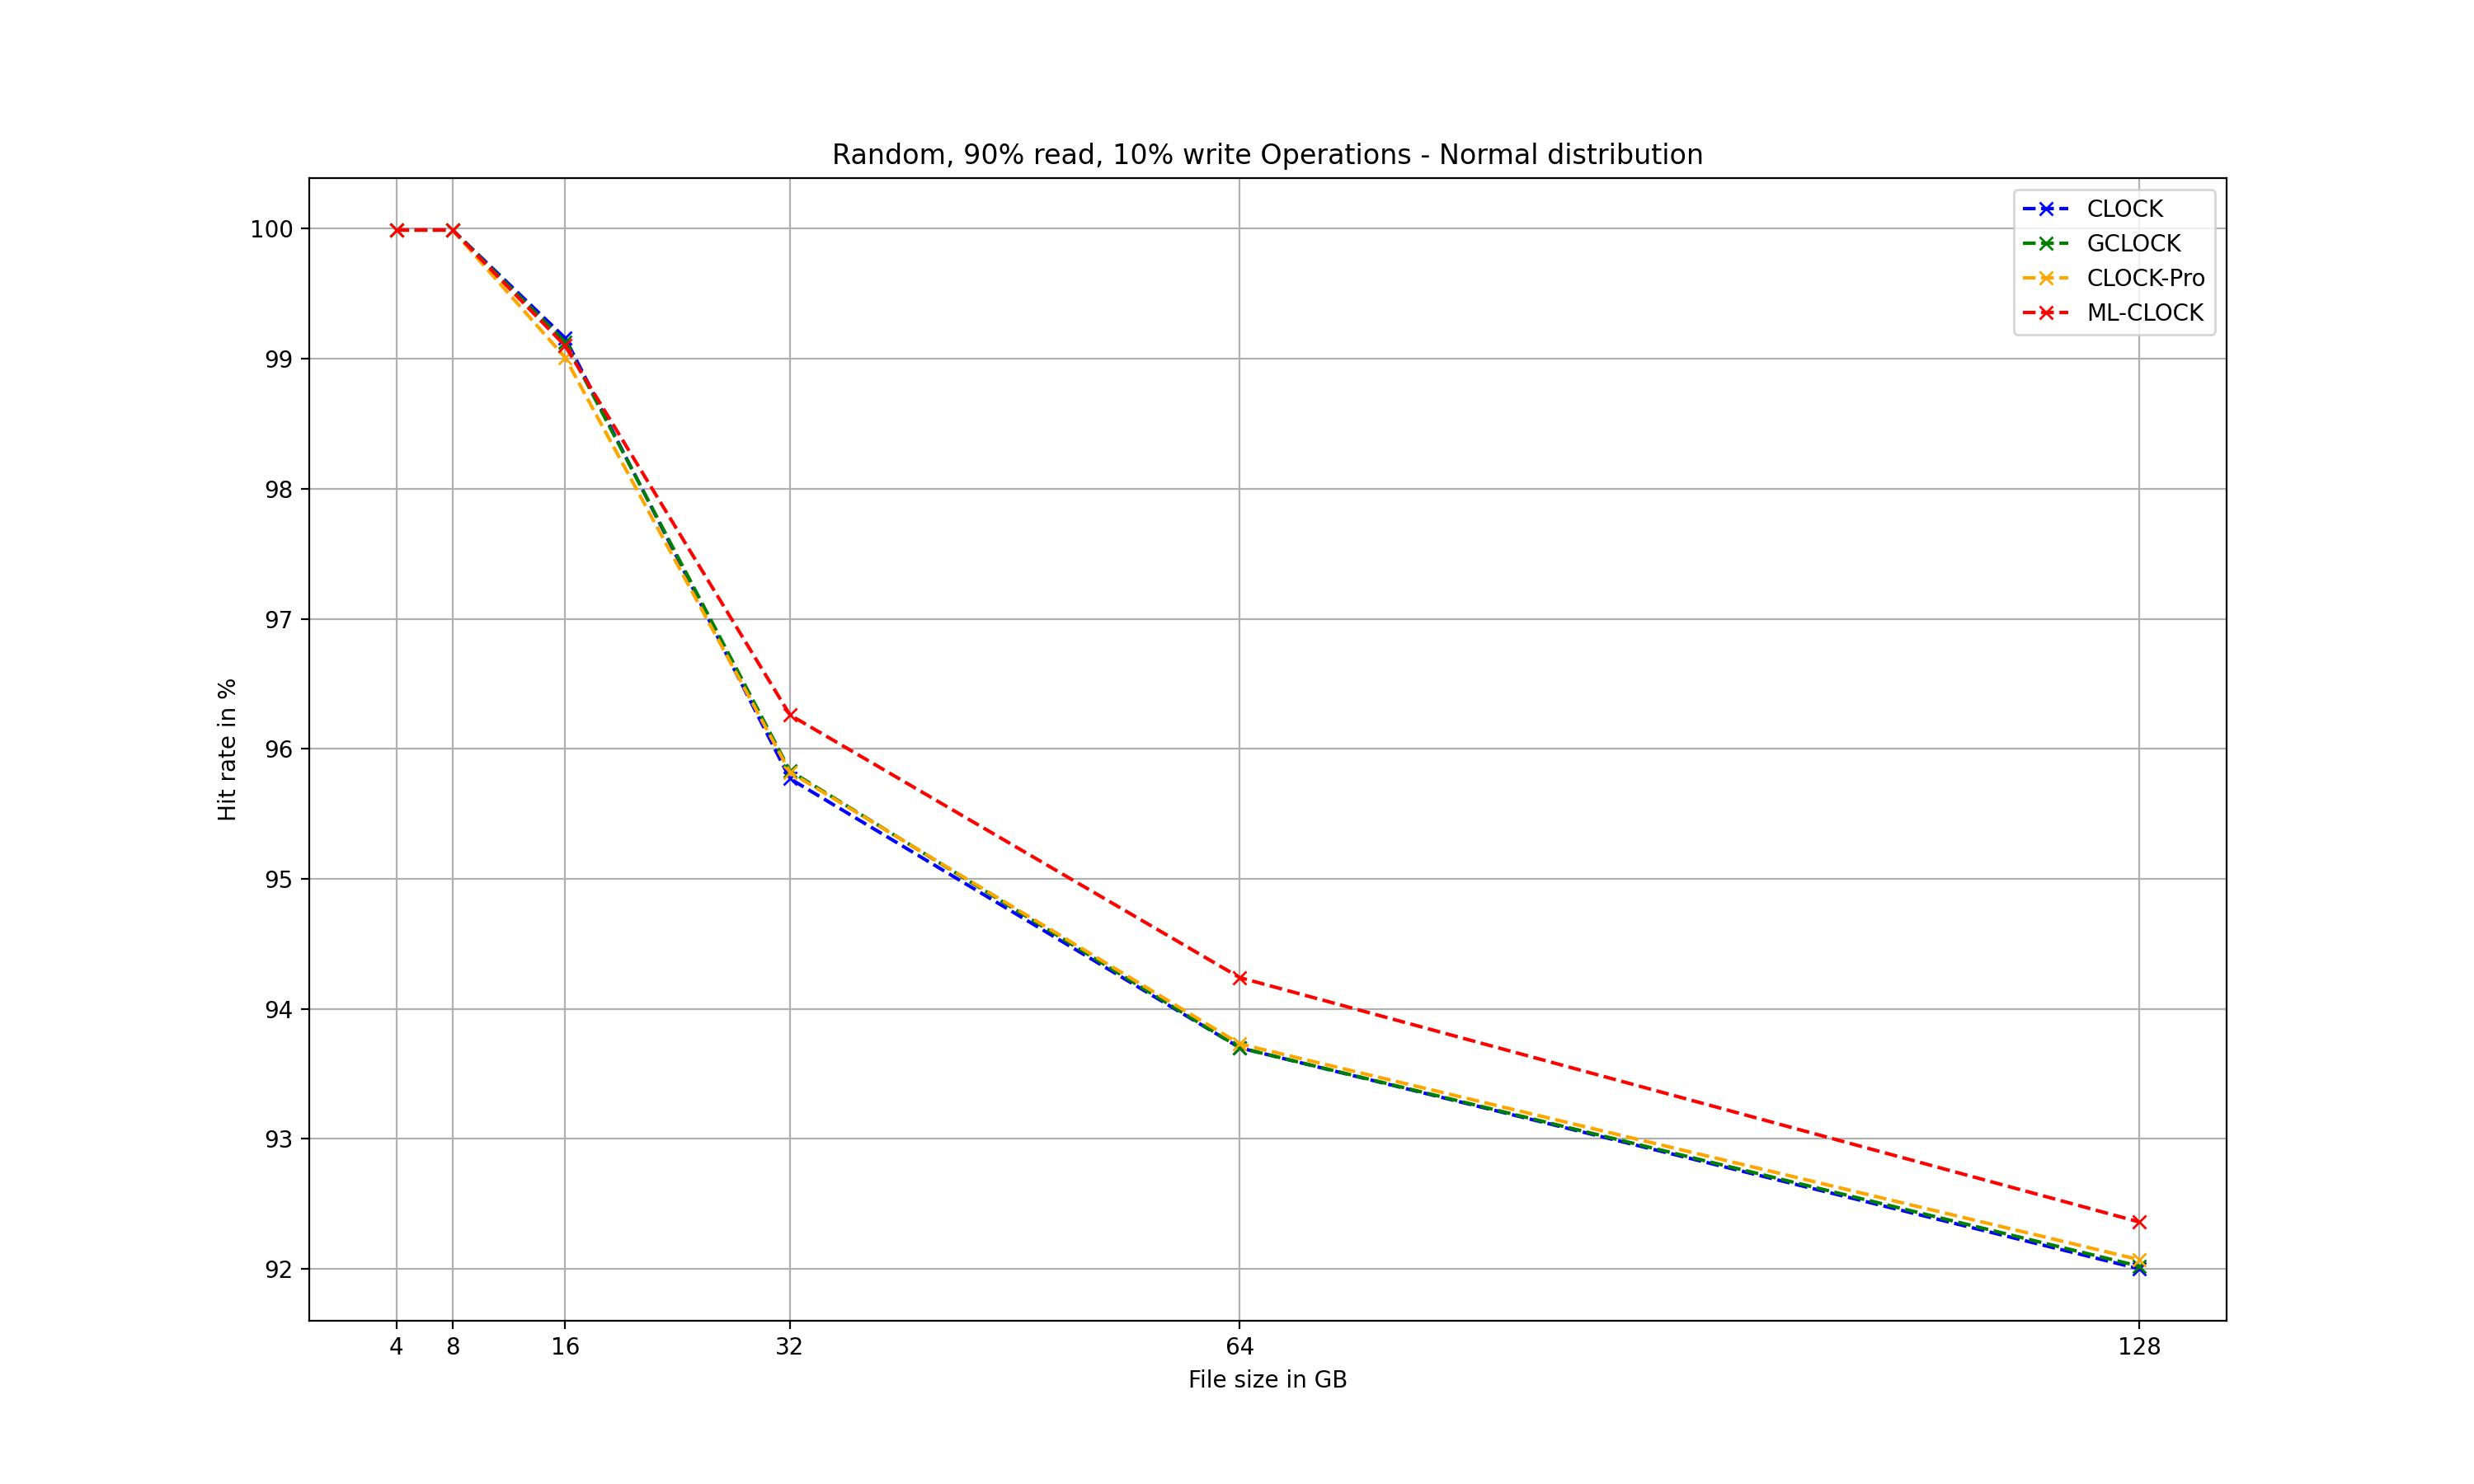
\includegraphics[width=\textwidth]{rw_90to10_normal.jpg}		
		\caption{Normal-distribution}
		\label{fig:rw_90to10  normal}
	\end{subfigure}
	\hfill
	\begin{subfigure}{0.4\textwidth}
		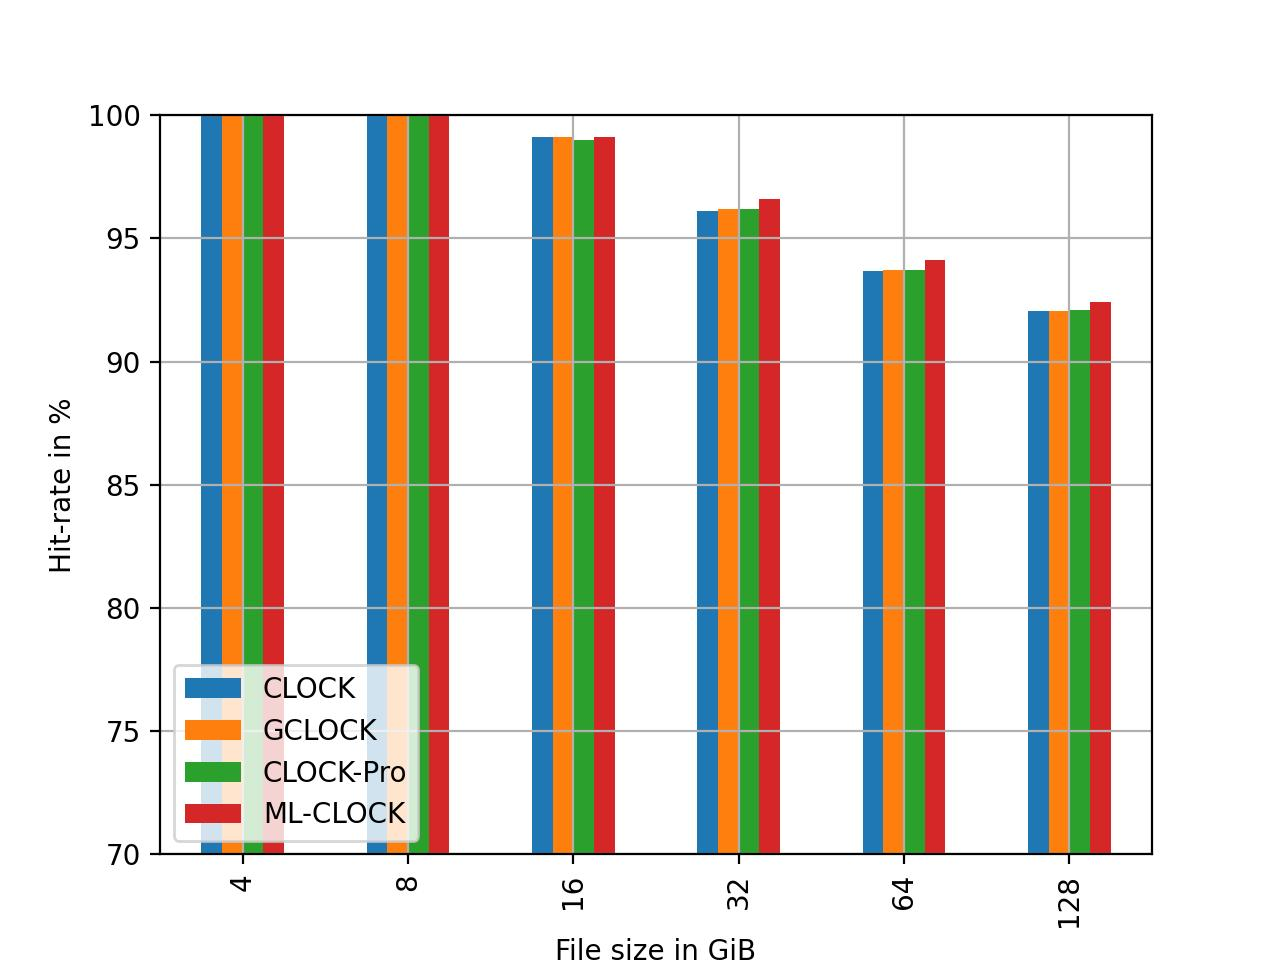
\includegraphics[width=\textwidth]{rw_90to10_zoned.jpg}		
		\caption{Zoned-distribution}
		\label{fig:rw_90to10  zoned}
	\end{subfigure}
	\hfill
	\begin{subfigure}{0.4\textwidth}
		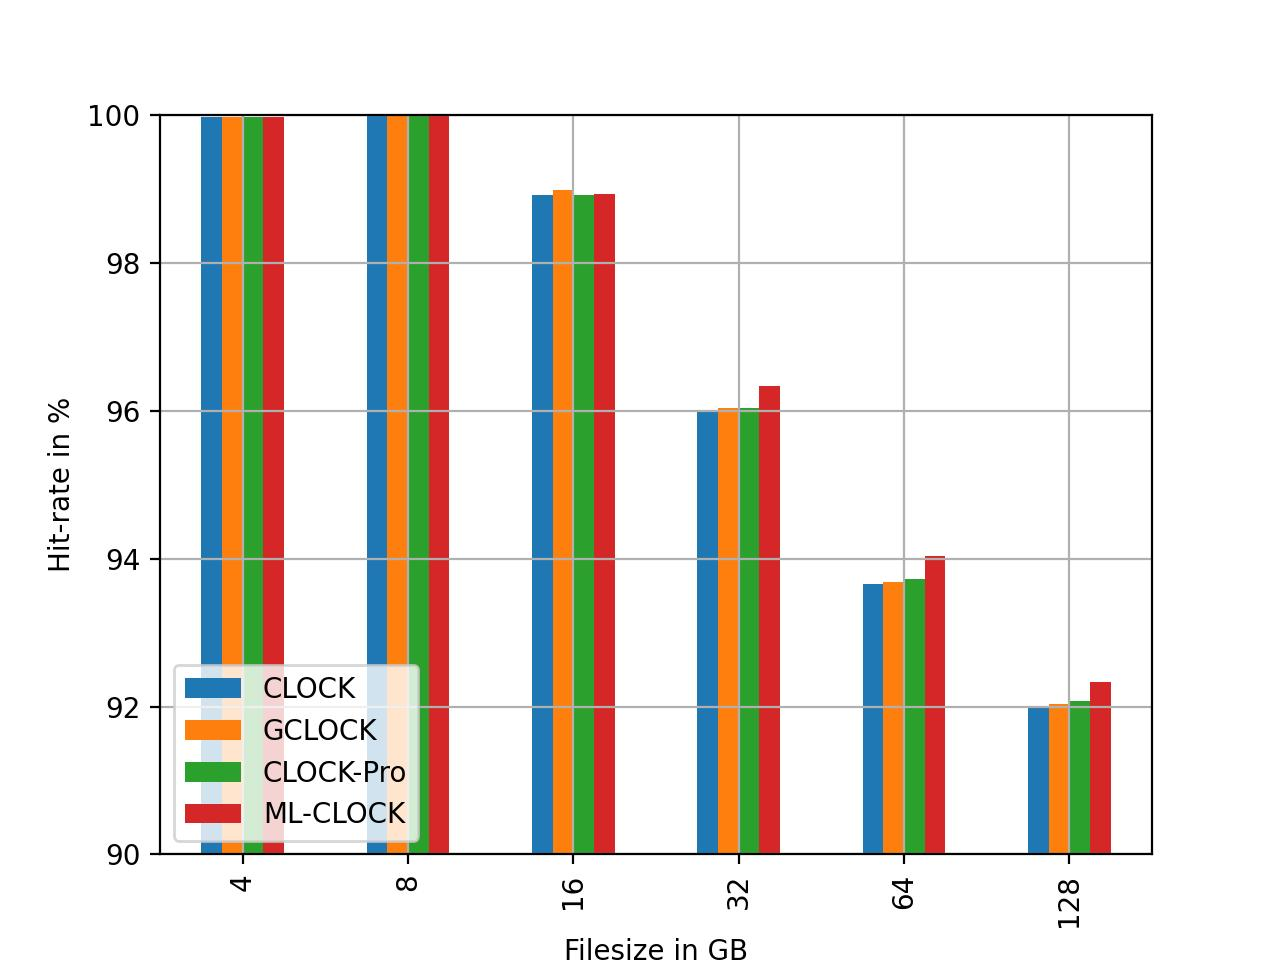
\includegraphics[width=\textwidth]{rw_90to10_uniform.jpg}		
		\caption{Uniform-distribution}
		\label{fig:rw_90to10  uniform}
	\end{subfigure}
	\caption{These figures show the hit-rate file-size diagram for each implemented 		cache replacement policy for random 90\% read 10\% write workload with different random distributions.}
\end{figure}

%-------------------------------------------------------

\begin{figure}[H]
	\centering
	\begin{subfigure}{0.4\textwidth}
		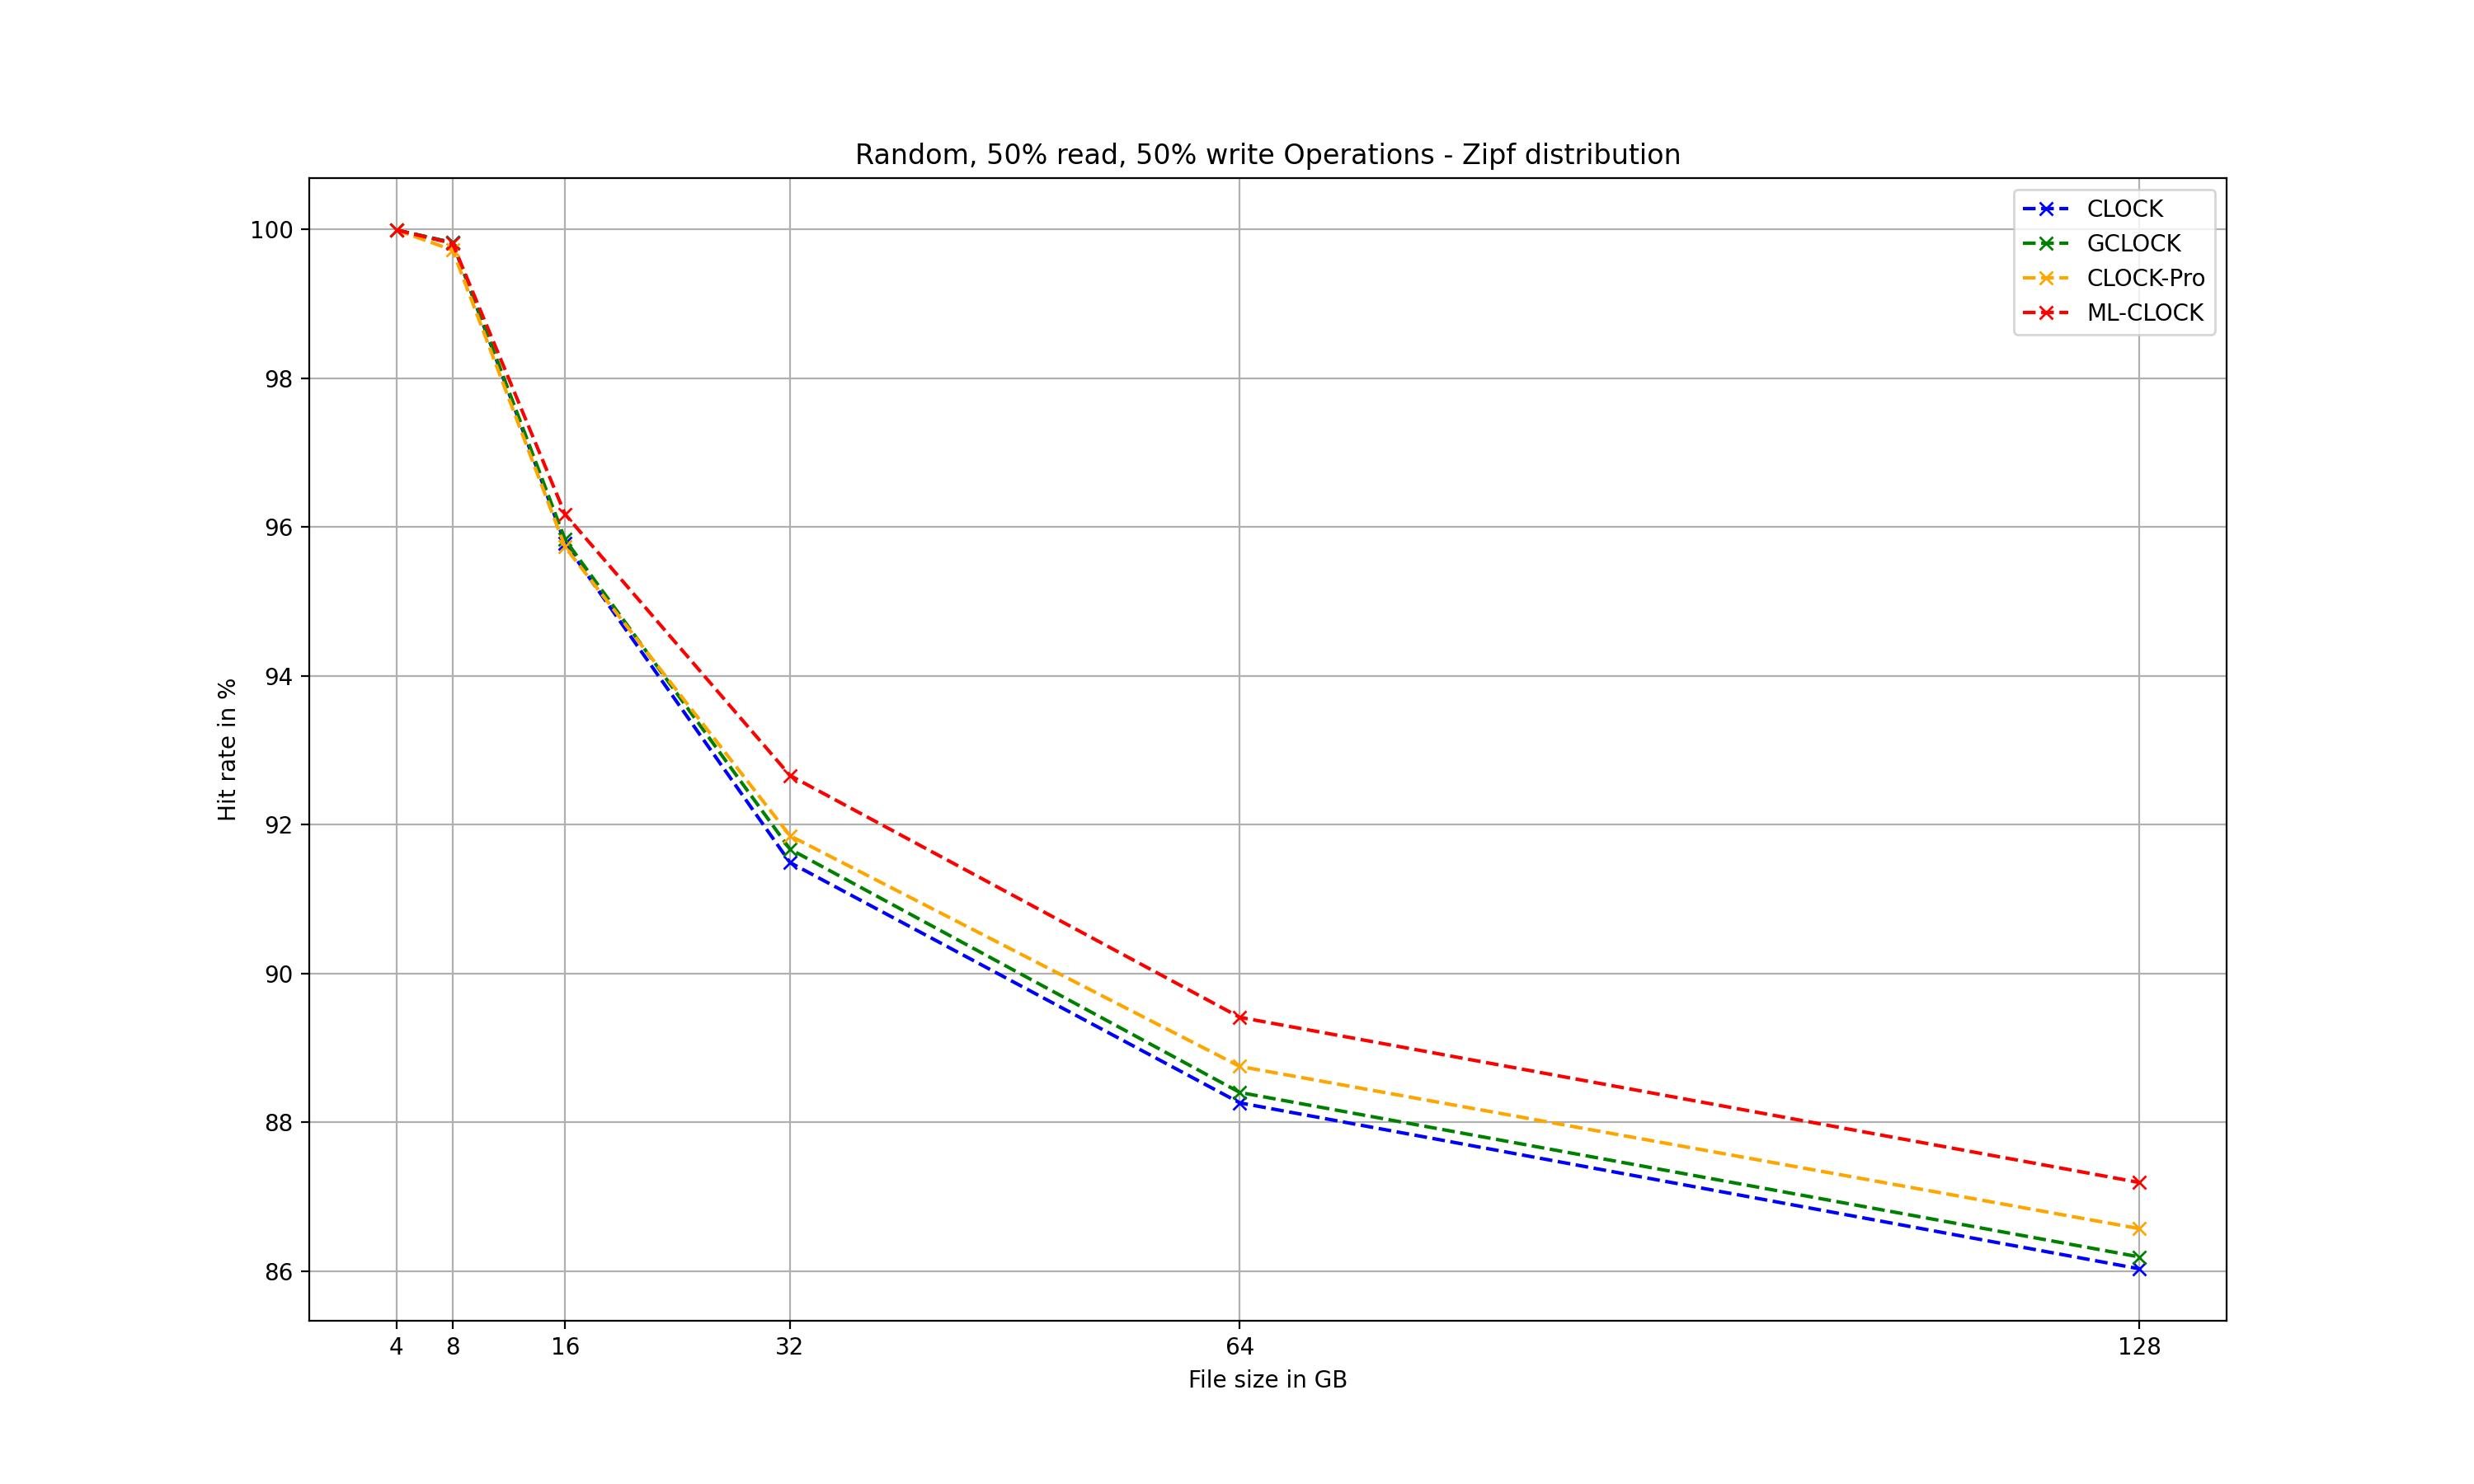
\includegraphics[width=\textwidth]{rw_50to50_zipf.jpg}		
		\caption{Zipf-distribution}
		\label{fig:rw_90to10  zipf}
	\end{subfigure}
	\hfill
	\begin{subfigure}{0.4\textwidth}
		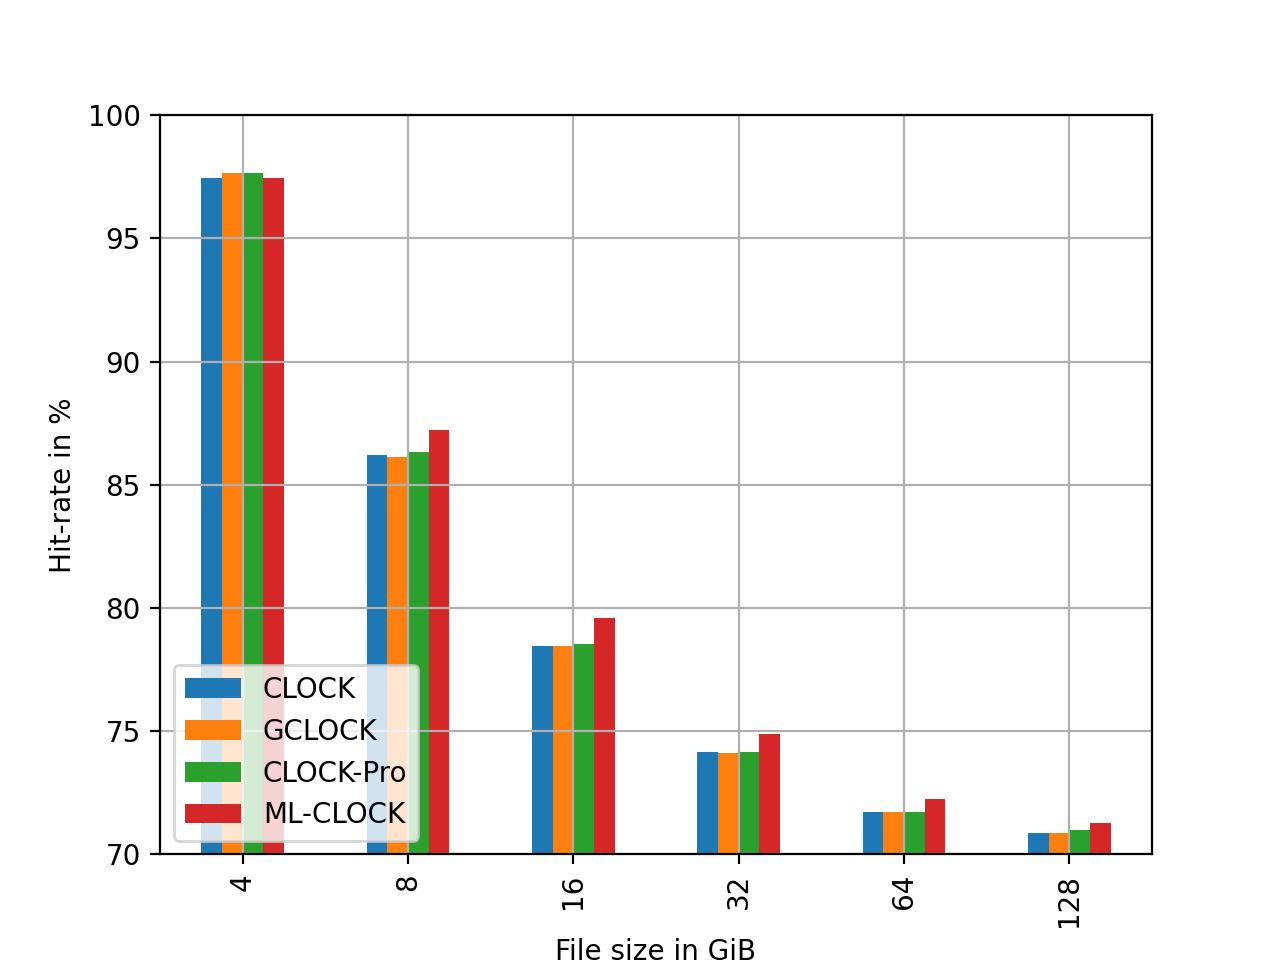
\includegraphics[width=\textwidth]{rw_50to50_normal.jpg}		
		\caption{Normal-distribution}
		\label{fig:rw_90to10  normal}
	\end{subfigure}
	\hfill
	\begin{subfigure}{0.4\textwidth}
		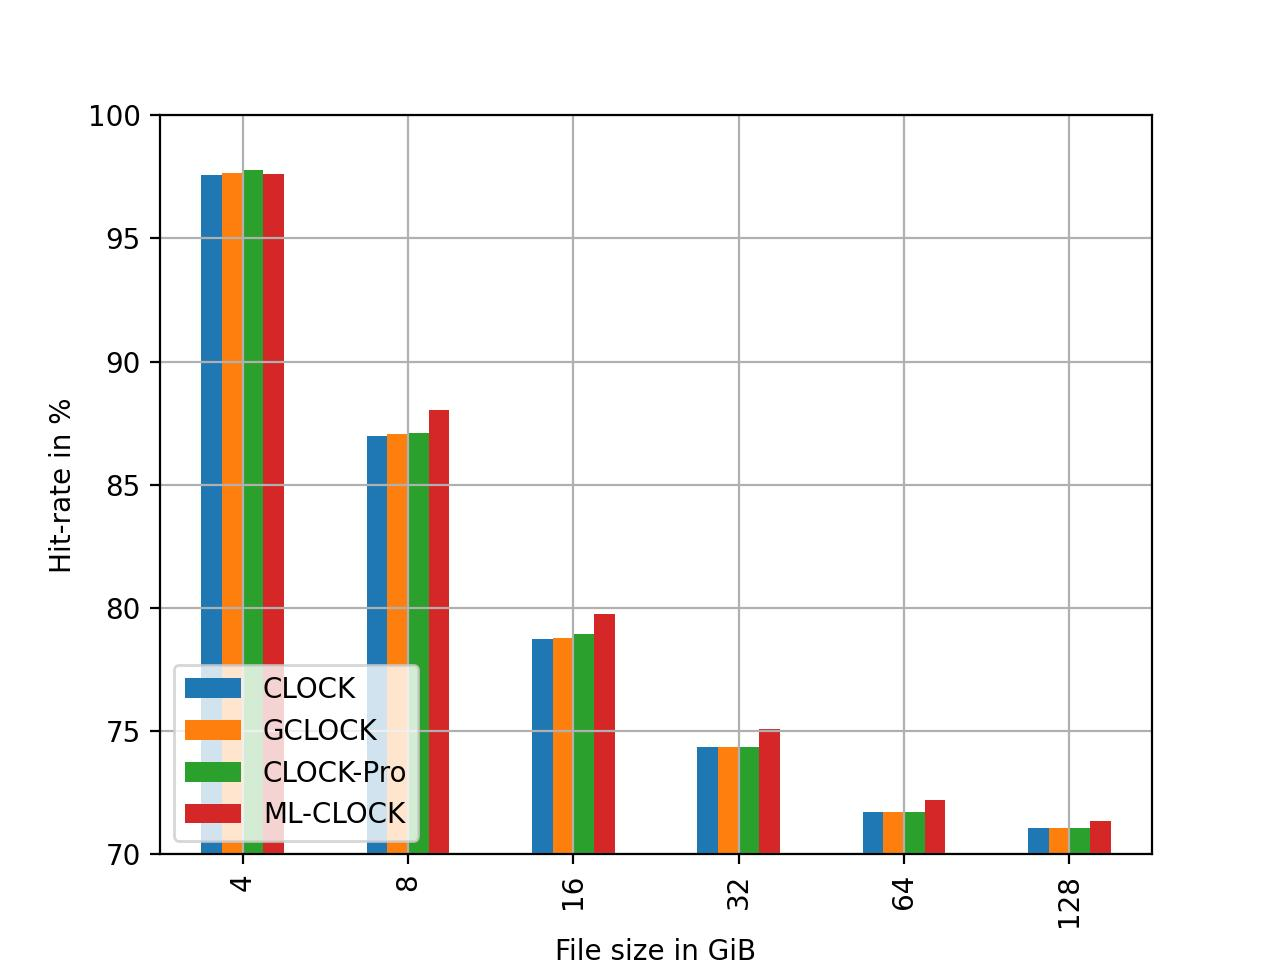
\includegraphics[width=\textwidth]{rw_50to50_zoned.jpg}		
		\caption{Zoned-distribution}
		\label{fig:rw_90to10  zoned}
	\end{subfigure}
	\hfill
	\begin{subfigure}{0.4\textwidth}
		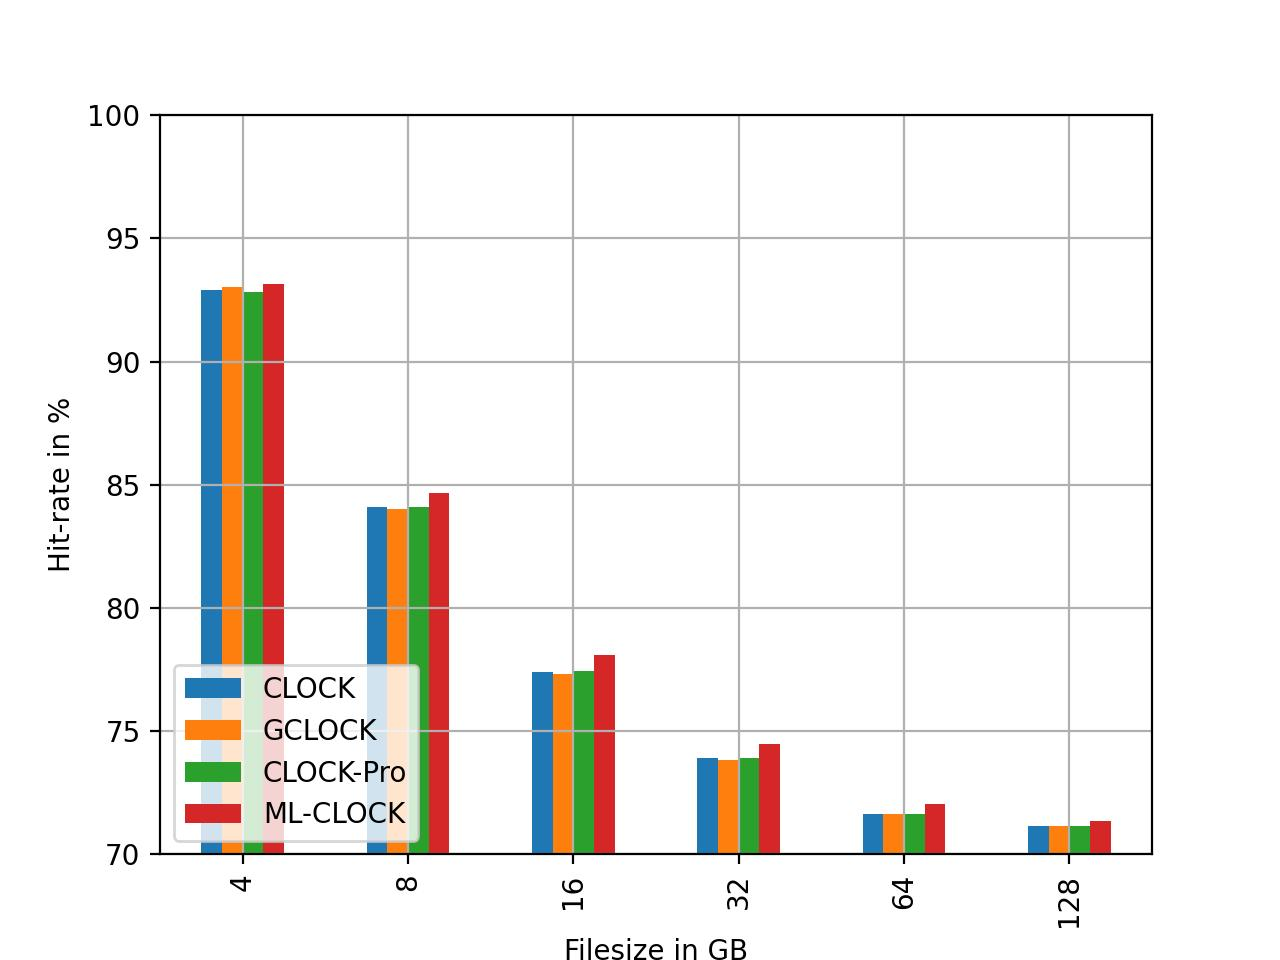
\includegraphics[width=\textwidth]{rw_50to50_uniform.jpg}		
		\caption{Uniform-distribution}
		\label{fig:rw_90to10  uniform}
	\end{subfigure}
	\caption{These figures show the hit-rate file-size diagram for each implemented 		cache replacement policy for random 50\% read 50\% write workload with different random distributions.}
\end{figure}

%-------------------------------------------------------

% not sure if I want to use this, don't have seq write for multi-threaded
\begin{figure}[H]
	\centering
	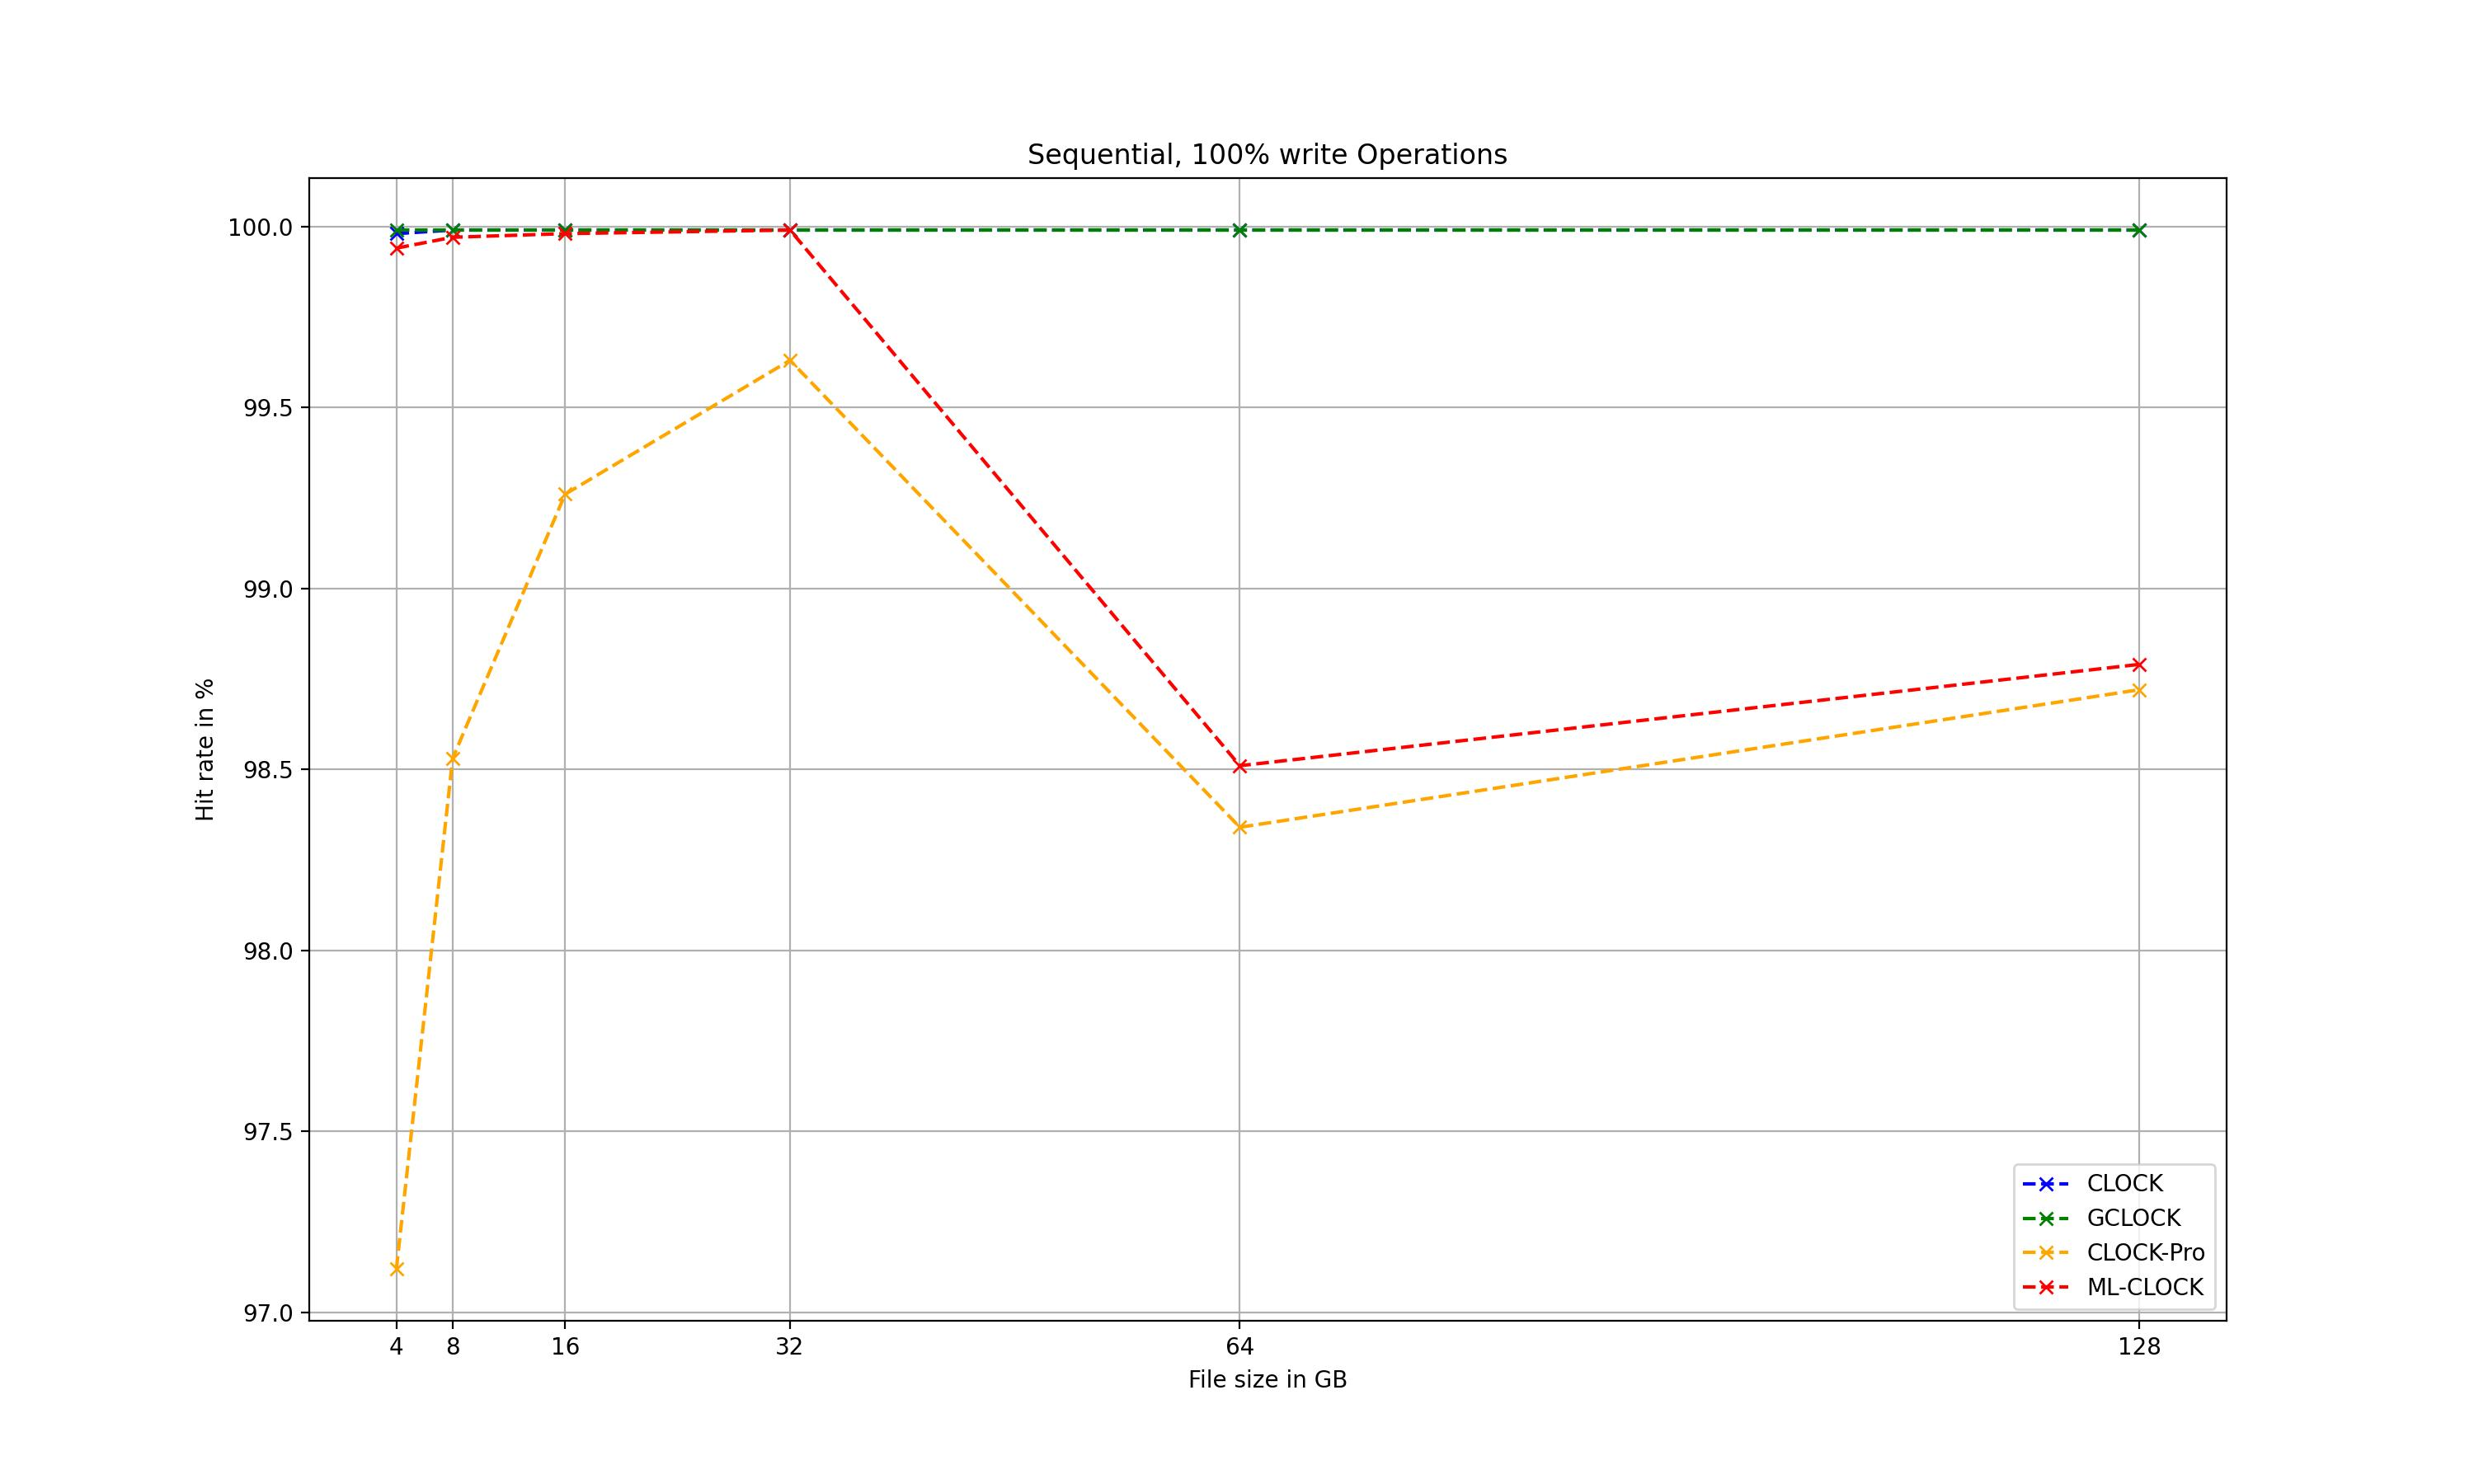
\includegraphics[scale=0.45]{seq_write.jpg}		
	\caption{This figure show the hit-rate file-size diagram for each implemented 		cache replacement policy for sequential writes}
	\label{fig:seq write}
\end{figure}


\section{Multi threaded}

- why the split of workloads

\subsection{Zipf-Distribution Workloads}
\begin{figure}[H]
	\centering
	\begin{subfigure}{0.4\textwidth}
		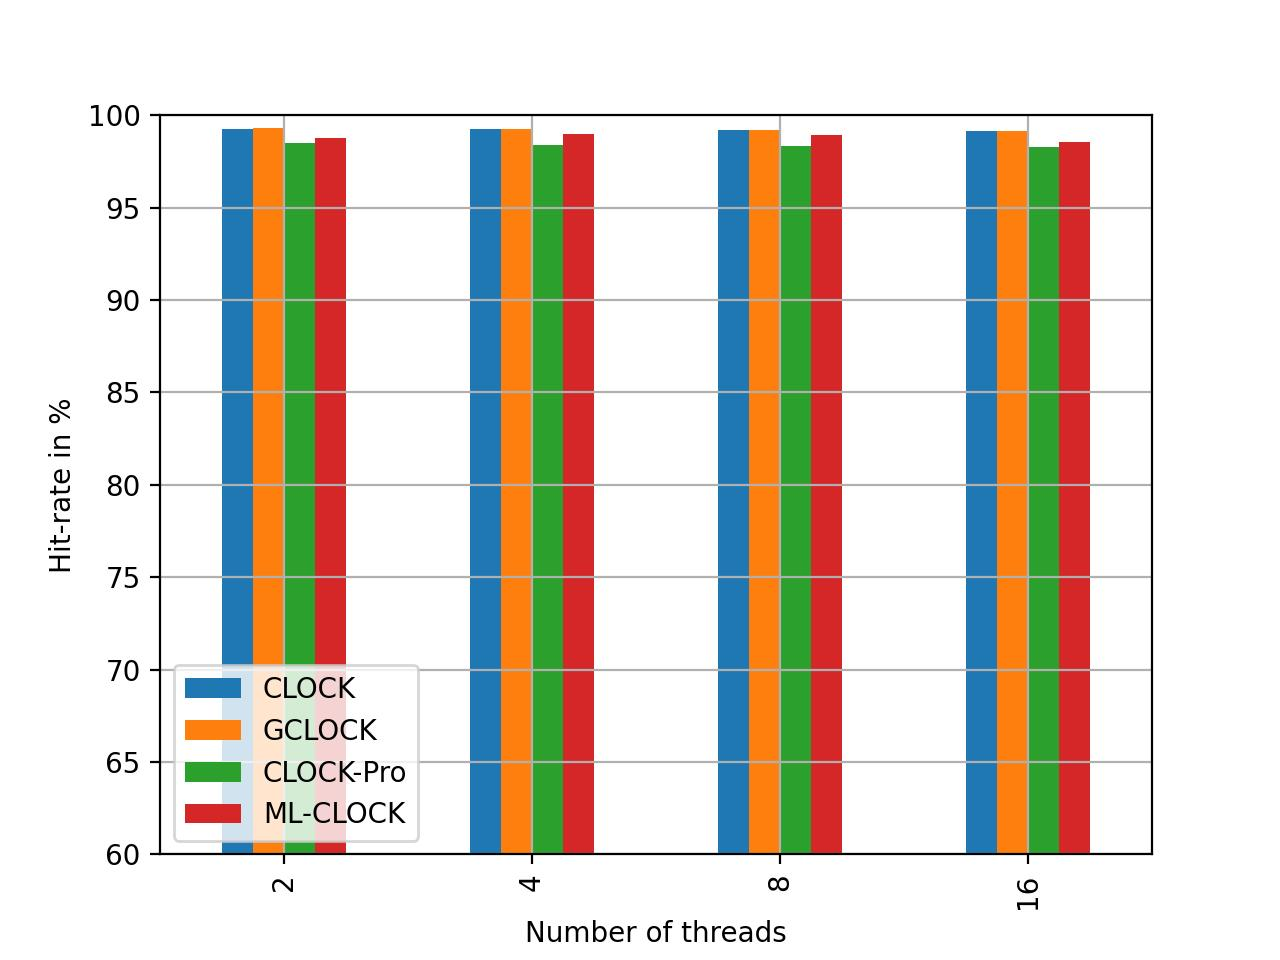
\includegraphics[width=\textwidth]{multi_16_gb_randread_zipf.jpg}		
		\caption{16 GiB file size}
		\label{fig:rw_90to10  zipf}
	\end{subfigure}
	\hfill
	\begin{subfigure}{0.4\textwidth}
		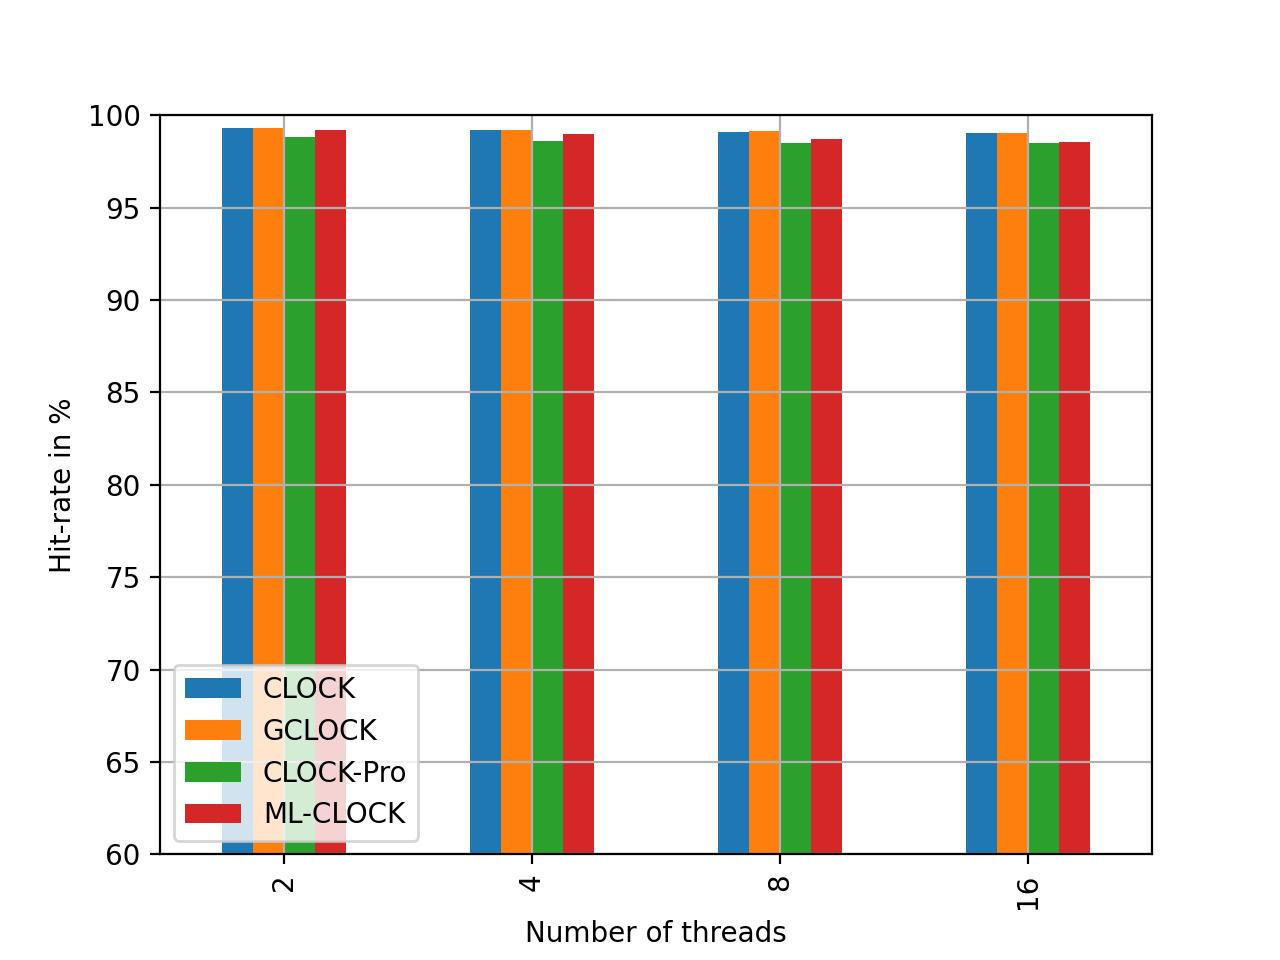
\includegraphics[width=\textwidth]{multi_32_gb_randread_zipf.jpg}		
		\caption{32 GiB file size}
		\label{fig:rw_90to10  normal}
	\end{subfigure}
	\hfill
	\begin{subfigure}{0.4\textwidth}
		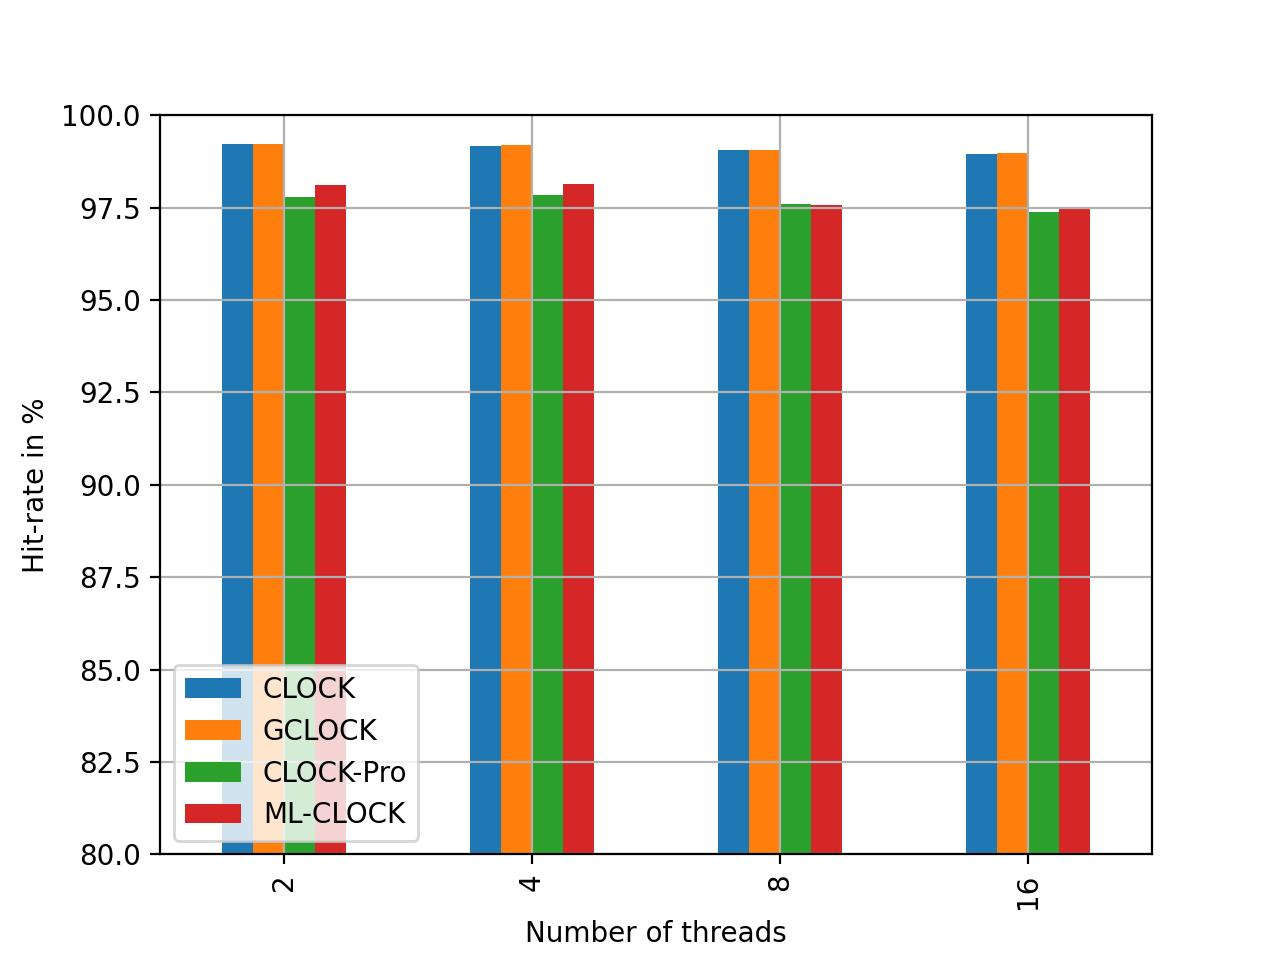
\includegraphics[width=\textwidth]{multi_64_gb_randread_zipf.jpg}		
		\caption{64 GiB file size}
		\label{fig:rw_90to10  zoned}
	\end{subfigure}
	\hfill
	\begin{subfigure}{0.4\textwidth}
		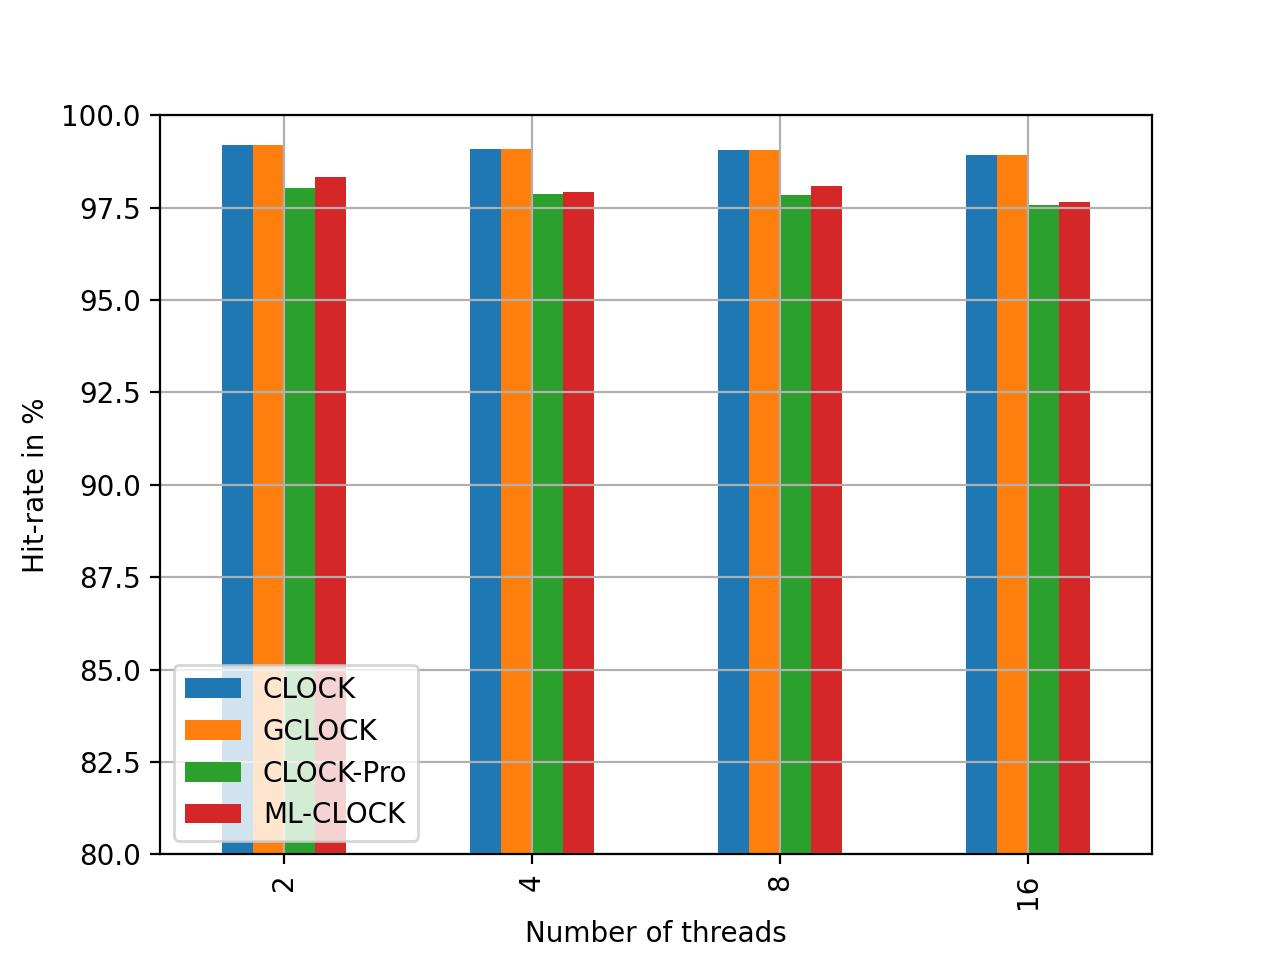
\includegraphics[width=\textwidth]{multi_128_gb_randread_zipf.jpg}		
		\caption{128 GiB file size}
		\label{fig:rw_90to10  uniform}
	\end{subfigure}
	\caption{These figures show the hit-rate for each implemented cache replacement policy for zipf-distribution random read only workload.}
\end{figure}

\begin{figure}[H]
	\centering
	\begin{subfigure}{0.4\textwidth}
		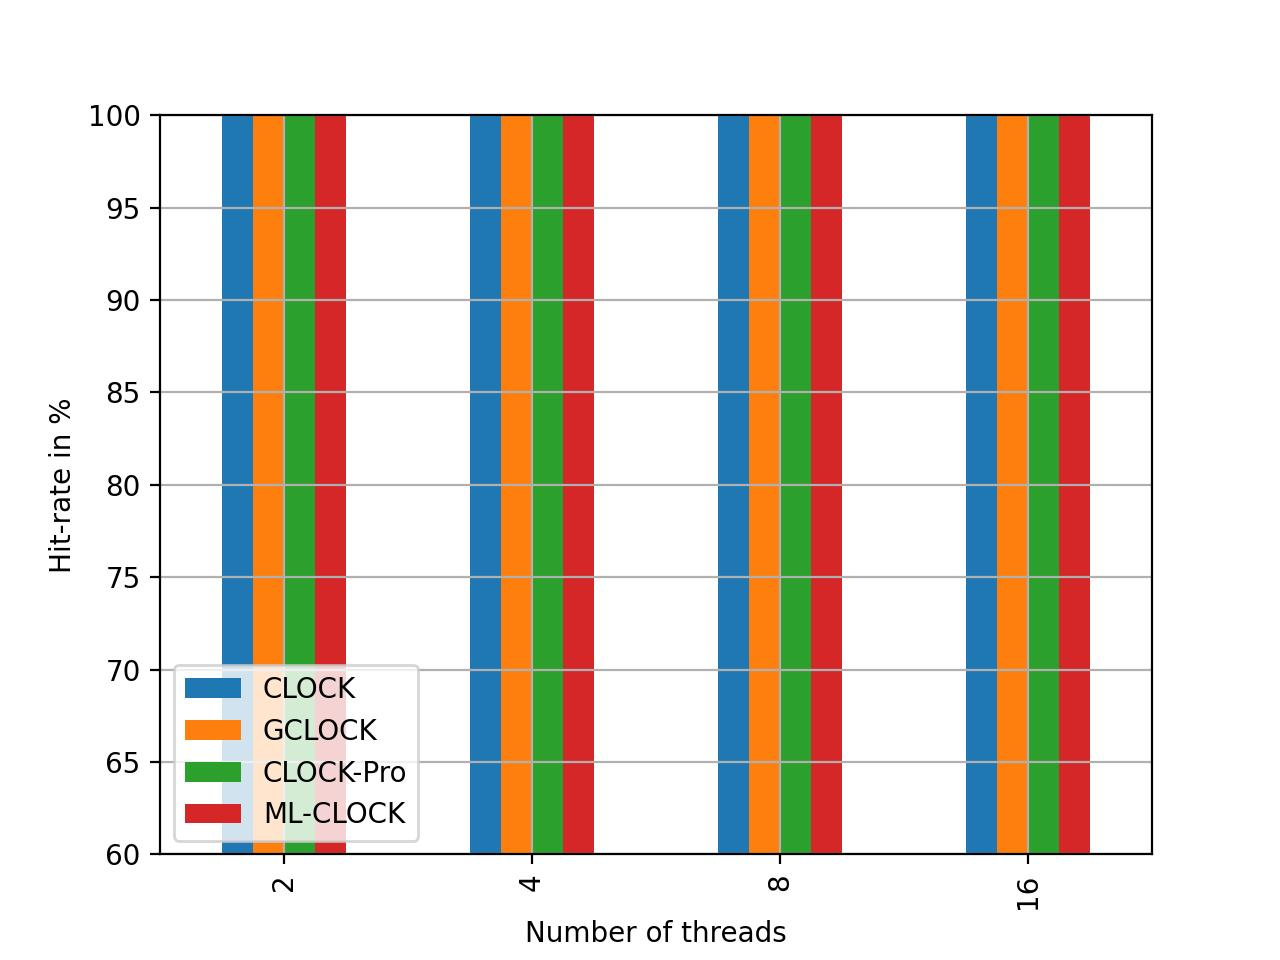
\includegraphics[width=\textwidth]{multi_16_gb_rw_90to10_zipf.jpg}		
		\caption{16 GiB file size}
		\label{fig:rw_90to10  zipf}
	\end{subfigure}
	\hfill
	\begin{subfigure}{0.4\textwidth}
		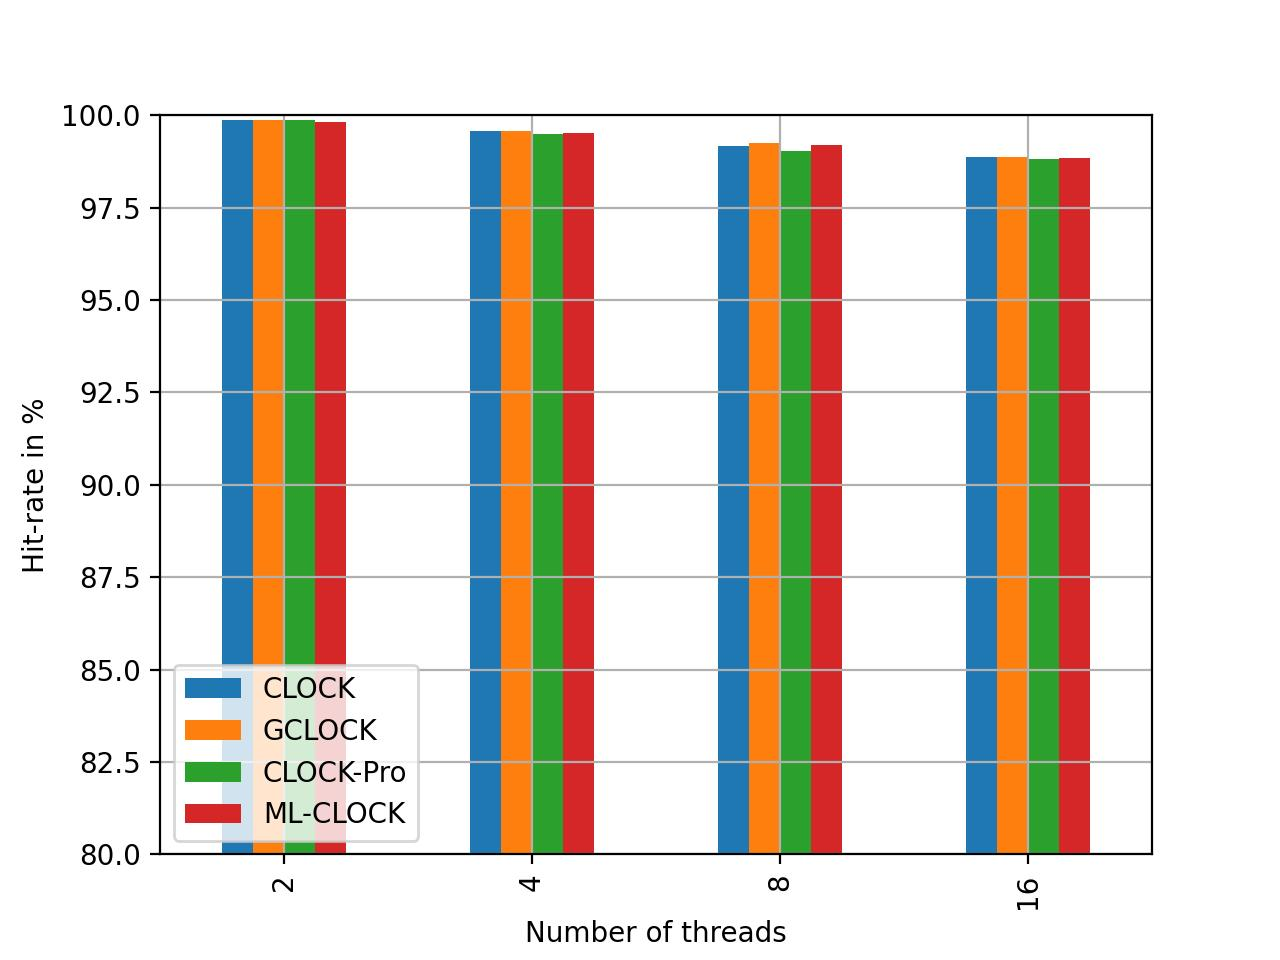
\includegraphics[width=\textwidth]{multi_32_gb_rw_90to10_zipf.jpg}		
		\caption{32 GiB file size}
		\label{fig:rw_90to10  normal}
	\end{subfigure}
	\hfill
	\begin{subfigure}{0.4\textwidth}
		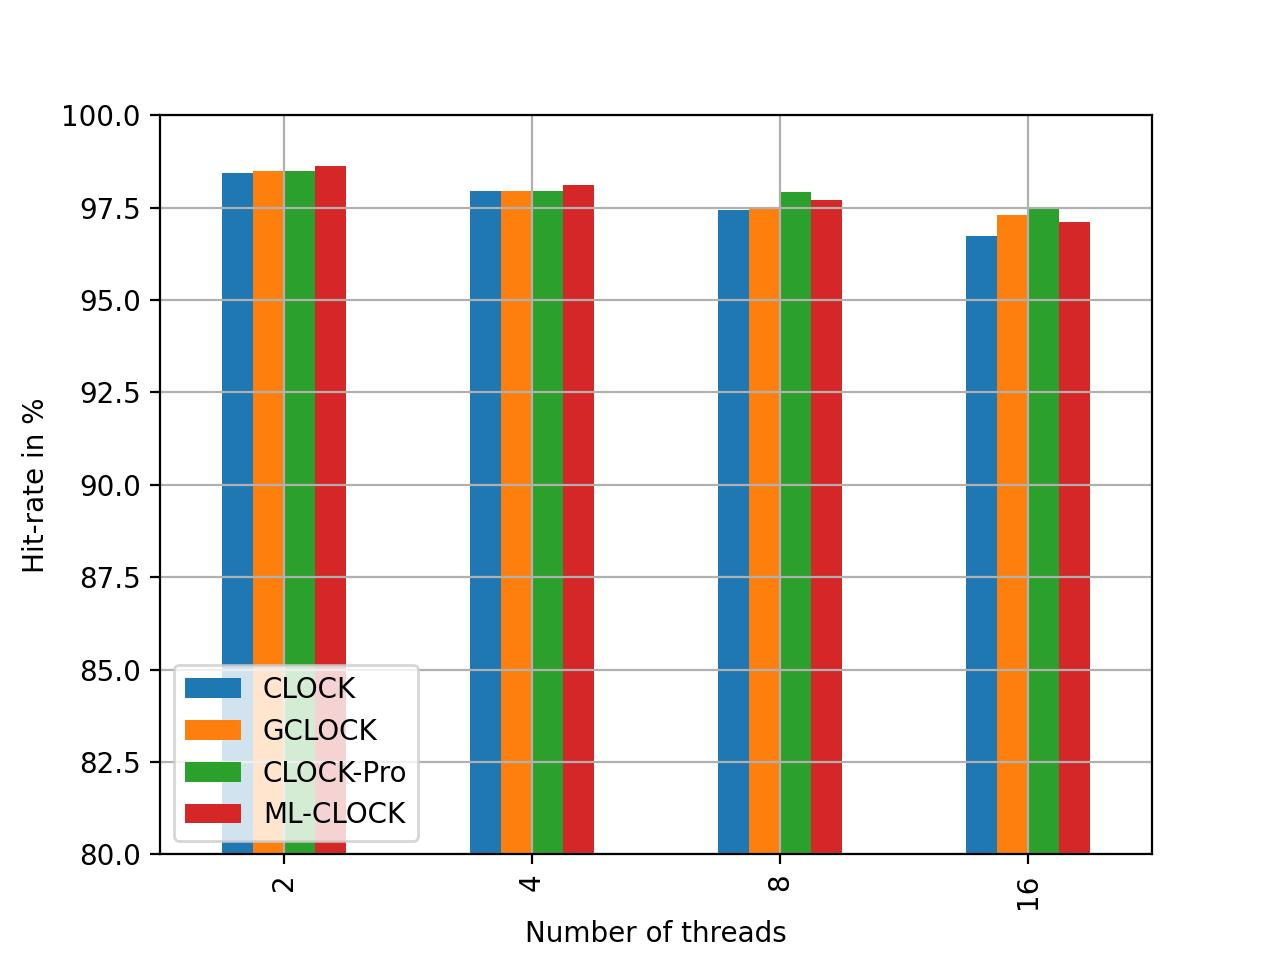
\includegraphics[width=\textwidth]{multi_64_gb_rw_90to10_zipf.jpg}		
		\caption{64 GiB file size}
		\label{fig:rw_90to10  zoned}
	\end{subfigure}
	\hfill
	\begin{subfigure}{0.4\textwidth}
		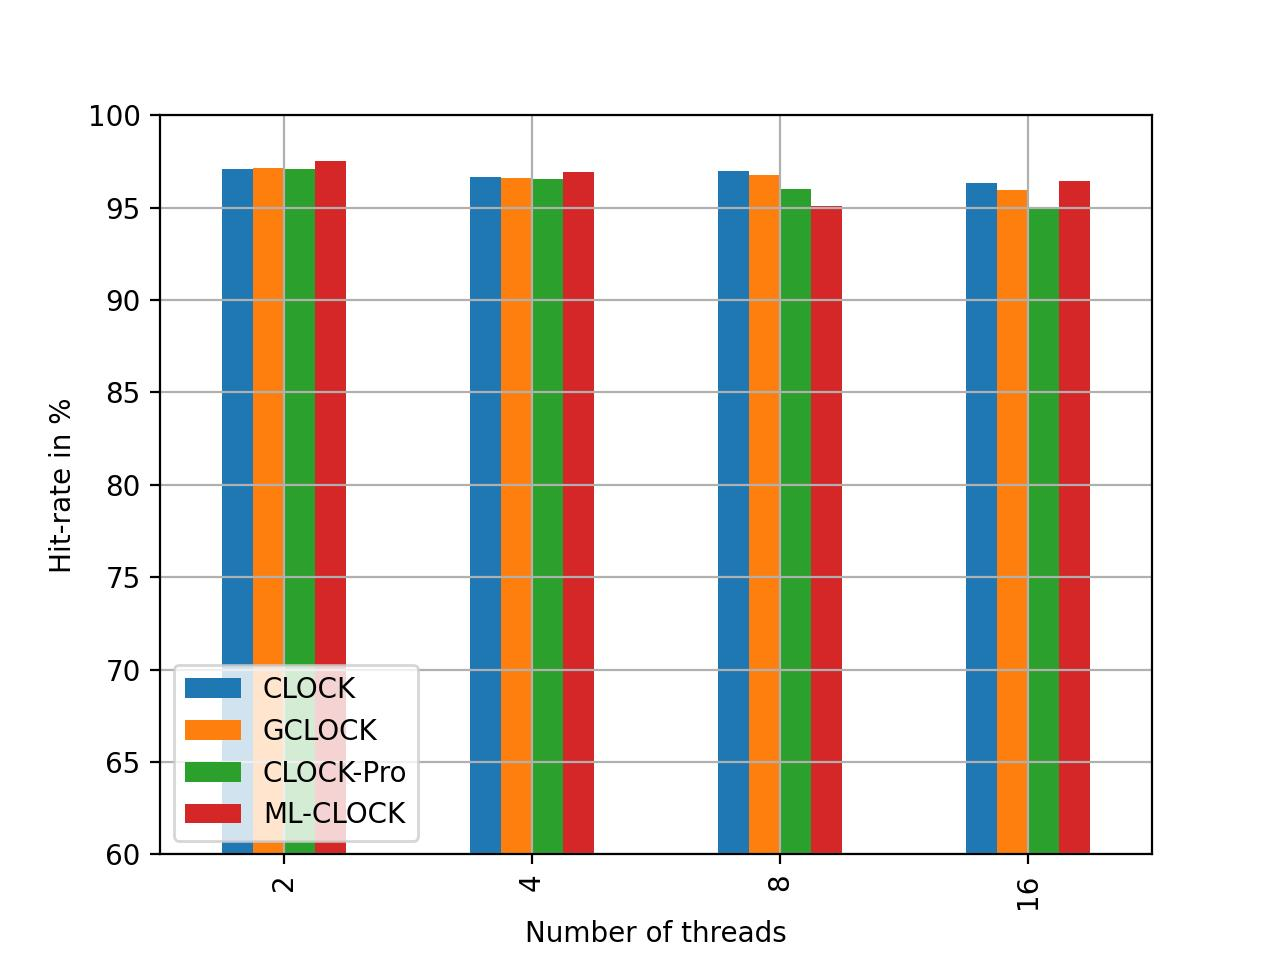
\includegraphics[width=\textwidth]{multi_128_gb_rw_90to10_zipf.jpg}		
		\caption{128 GiB file size}
		\label{fig:rw_90to10  uniform}
	\end{subfigure}
	\caption{These figures show the hit-rate for each implemented cache replacement policy for zipf-distribution random 90\% read 10\% write workload.}
\end{figure}

\begin{figure}[H]
	\centering
	\begin{subfigure}{0.4\textwidth}
		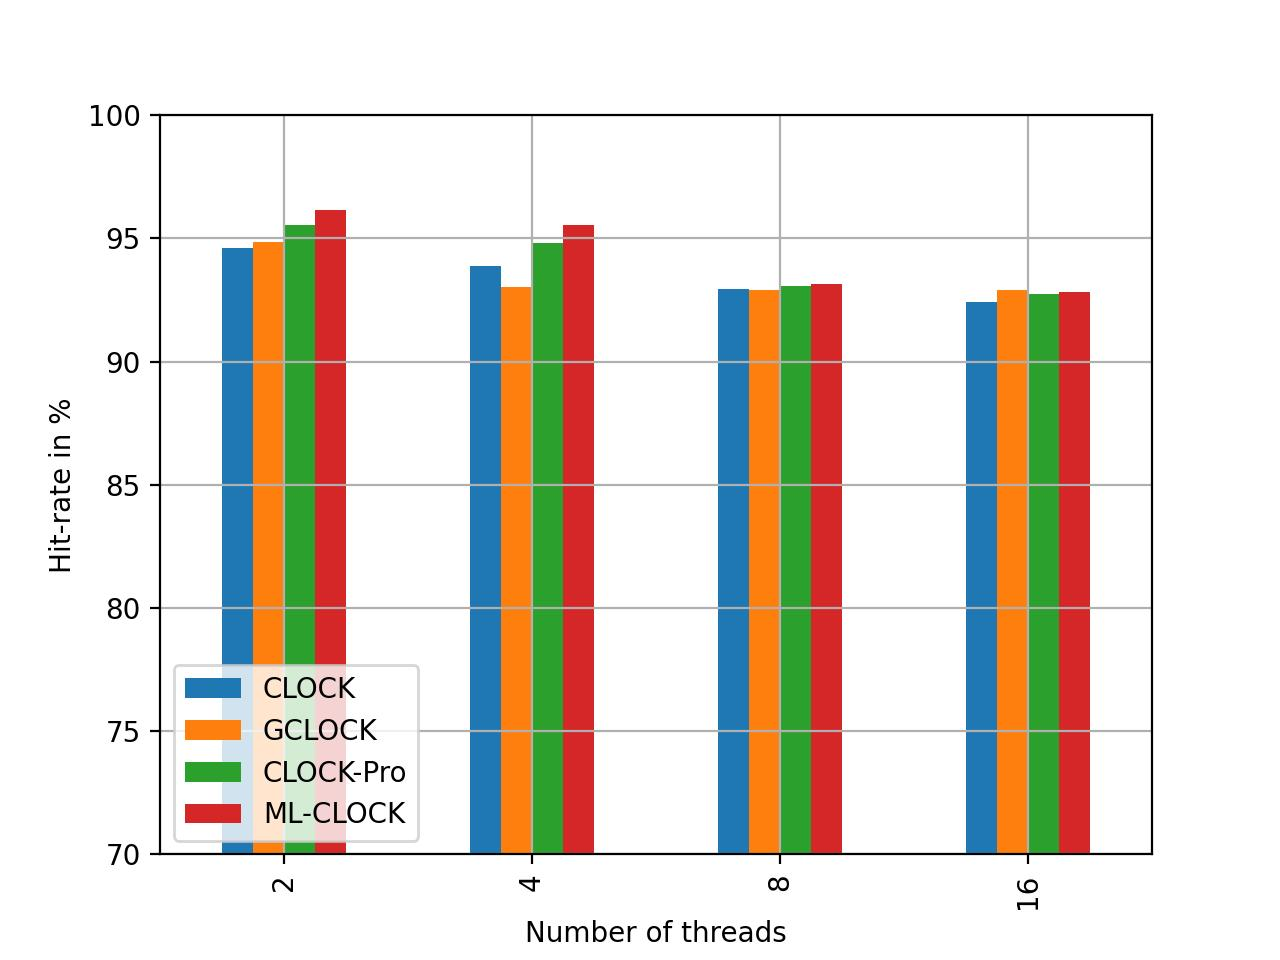
\includegraphics[width=\textwidth]{multi_16_gb_rw_50to50_zipf.jpg}		
		\caption{16 GiB file size}
		\label{fig:rw_90to10  zipf}
	\end{subfigure}
	\hfill
	\begin{subfigure}{0.4\textwidth}
		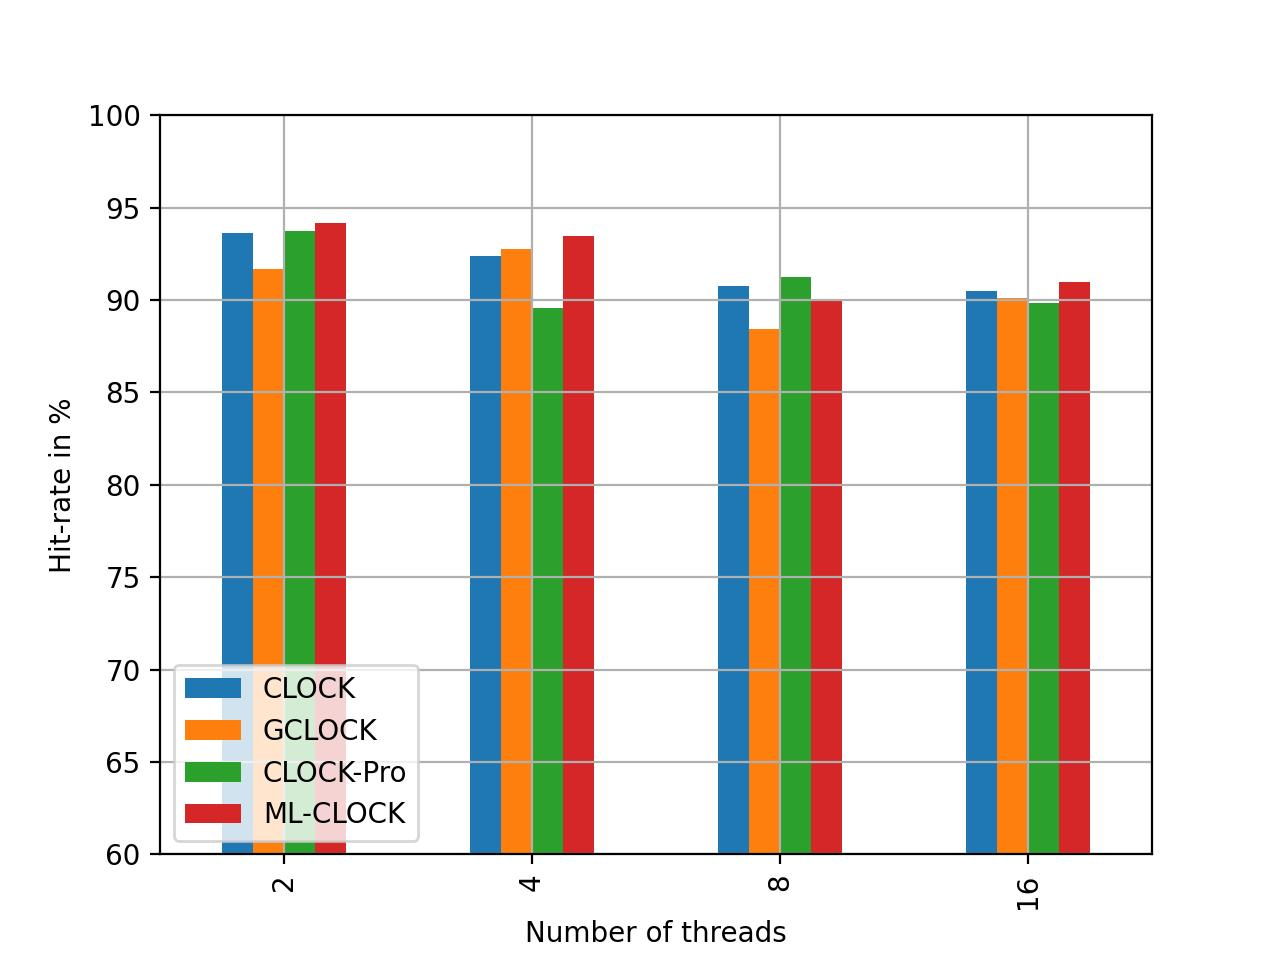
\includegraphics[width=\textwidth]{multi_32_gb_rw_50to50_zipf.jpg}		
		\caption{32 GiB file size}
		\label{fig:rw_90to10  normal}
	\end{subfigure}
	\hfill
	\begin{subfigure}{0.4\textwidth}
		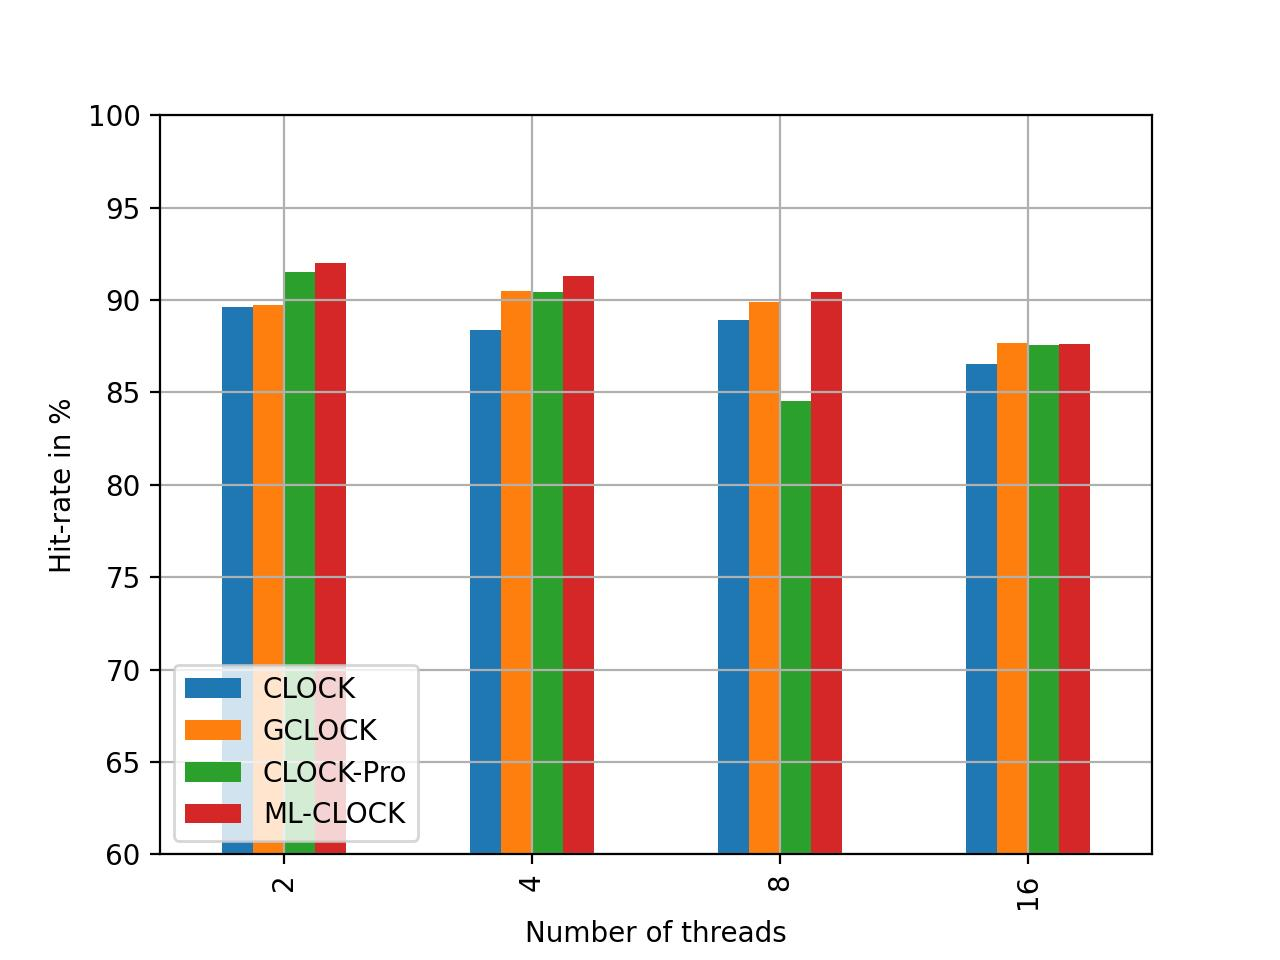
\includegraphics[width=\textwidth]{multi_64_gb_rw_50to50_zipf.jpg}		
		\caption{64 GiB file size}
		\label{fig:rw_90to10  zoned}
	\end{subfigure}
	\hfill
	\begin{subfigure}{0.4\textwidth}
		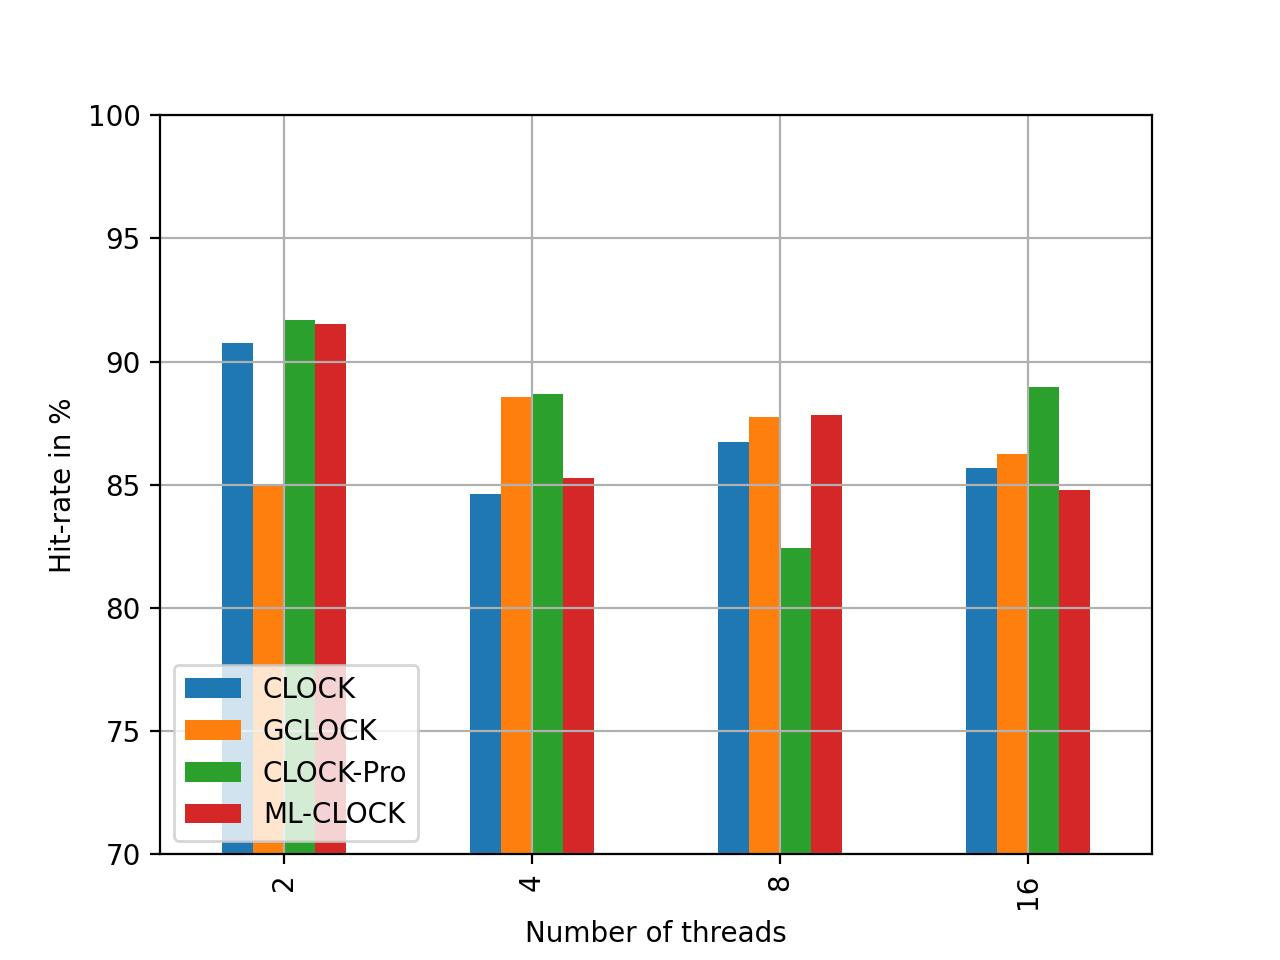
\includegraphics[width=\textwidth]{multi_128_gb_rw_50to50_zipf.jpg}		
		\caption{128 GiB file size}
		\label{fig:rw_90to10  uniform}
	\end{subfigure}
	\caption{These figures show the hit-rate for each implemented cache replacement policy for normal-distribution random 50\% read 50\% write workload.}
\end{figure}

%----------------------------------------------

\subsection{Normal-Distribution Workloads}
\begin{figure}[H]
	\centering
	\begin{subfigure}{0.4\textwidth}
		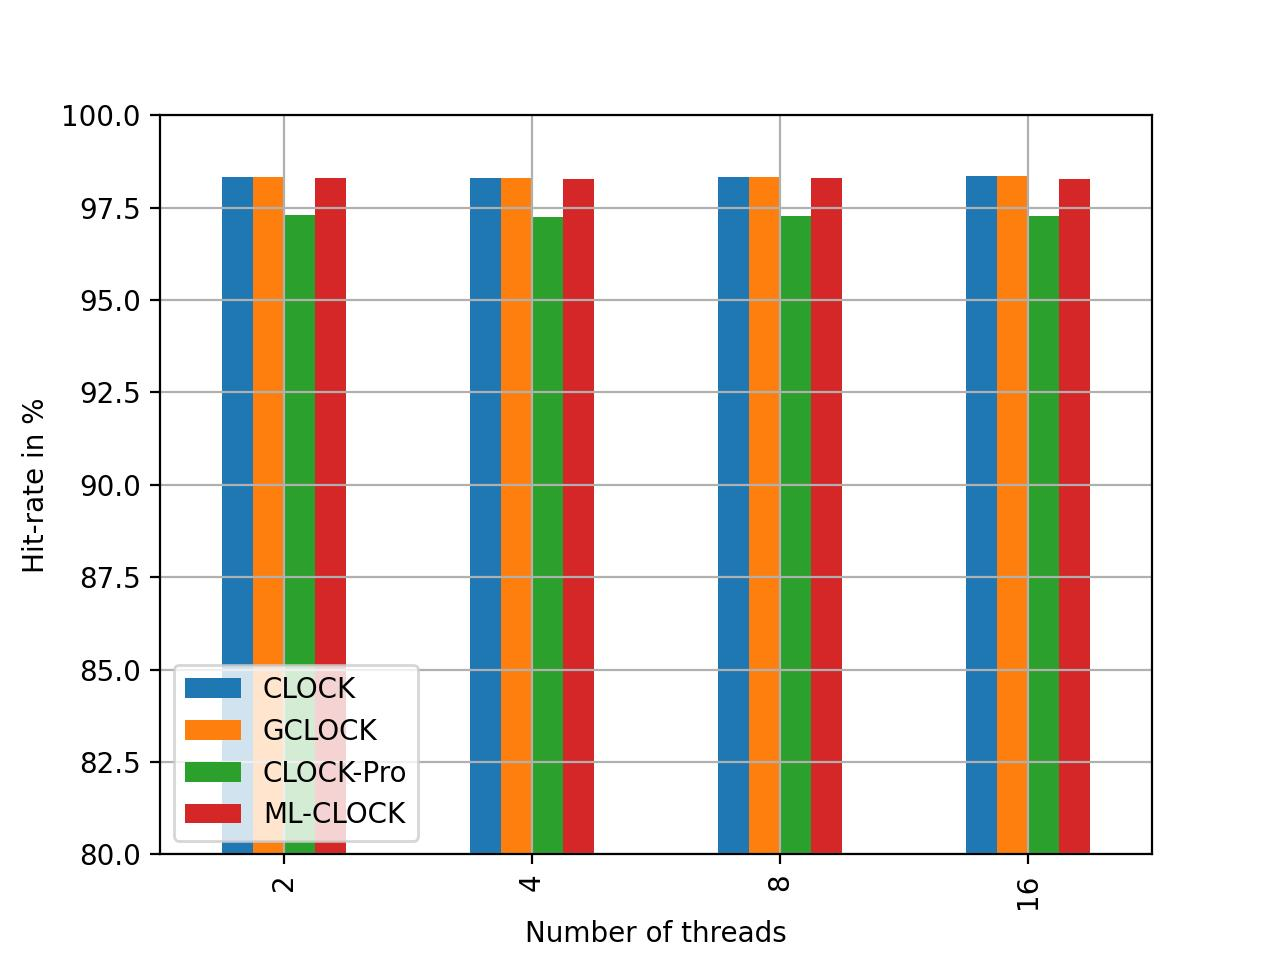
\includegraphics[width=\textwidth]{multi_16_gb_randread_normal.jpg}		
		\caption{16 GiB file size}
		\label{fig:rw_90to10  zipf}
	\end{subfigure}
	\hfill
	\begin{subfigure}{0.4\textwidth}
		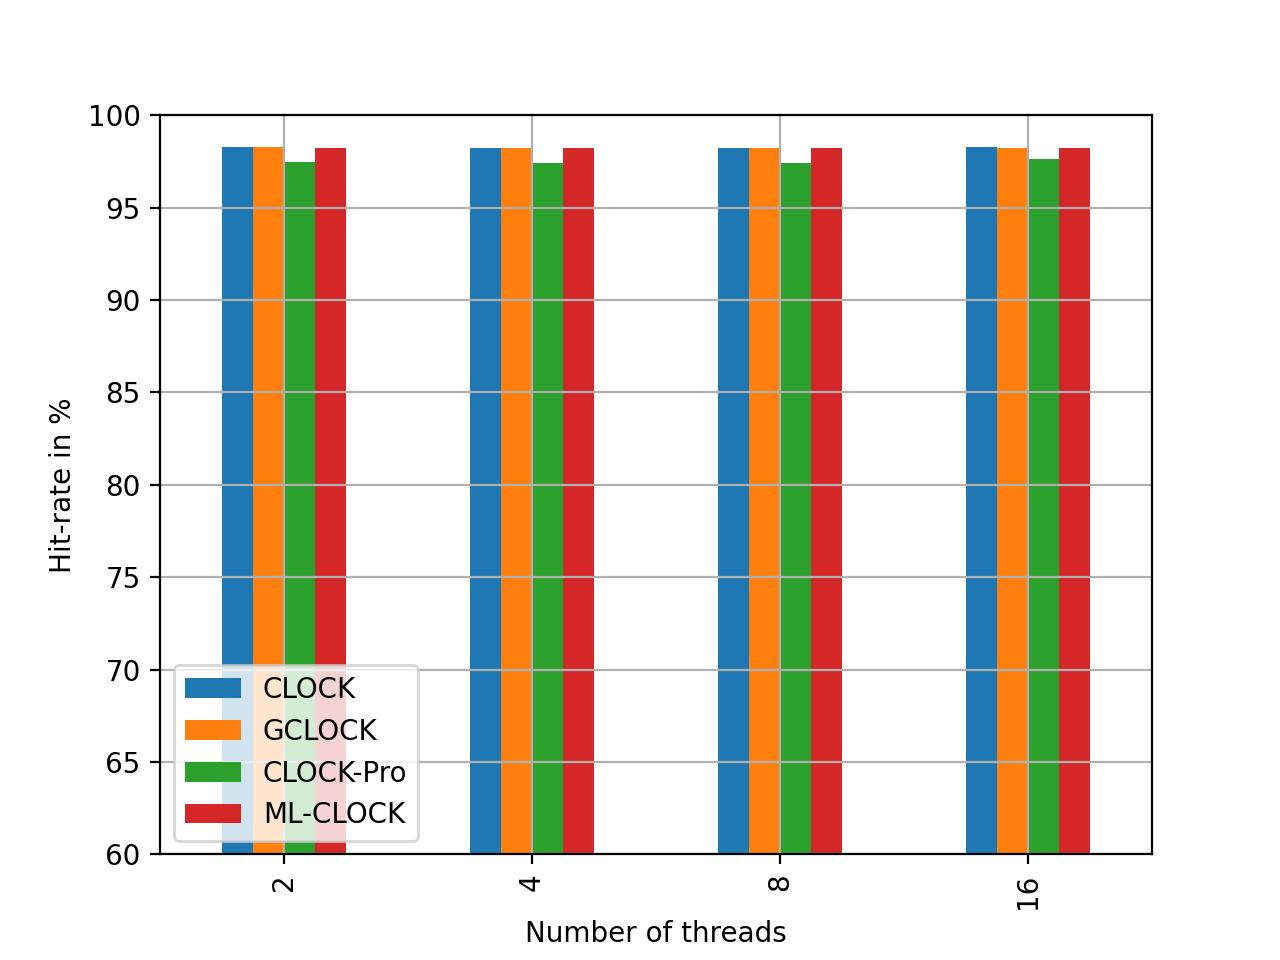
\includegraphics[width=\textwidth]{multi_32_gb_randread_normal.jpg}		
		\caption{32 GiB file size}
		\label{fig:rw_90to10  normal}
	\end{subfigure}
	\hfill
	\begin{subfigure}{0.4\textwidth}
		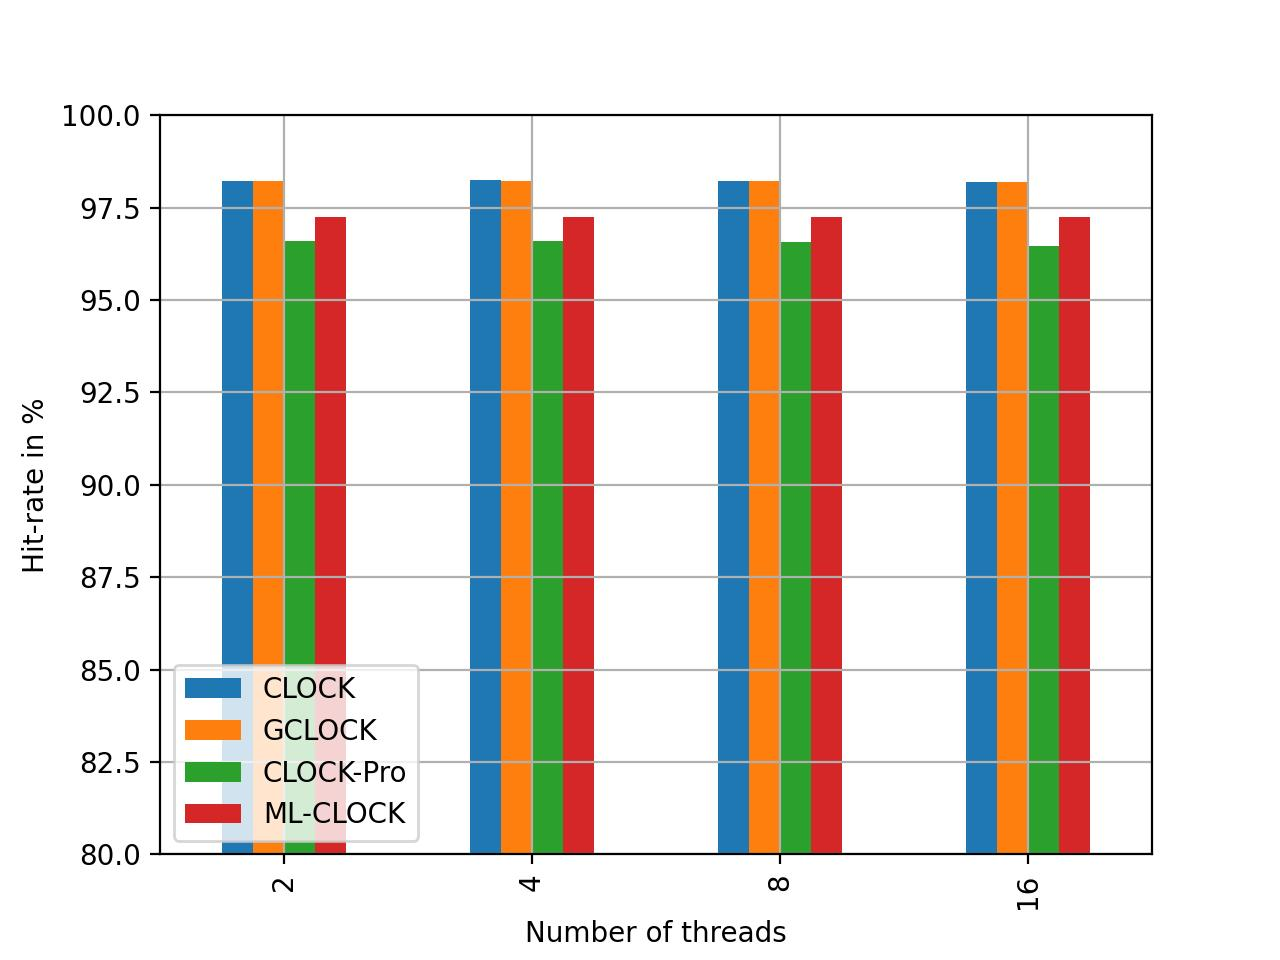
\includegraphics[width=\textwidth]{multi_64_gb_randread_normal.jpg}		
		\caption{64 GiB file size}
		\label{fig:rw_90to10  zoned}
	\end{subfigure}
	\hfill
	\begin{subfigure}{0.4\textwidth}
		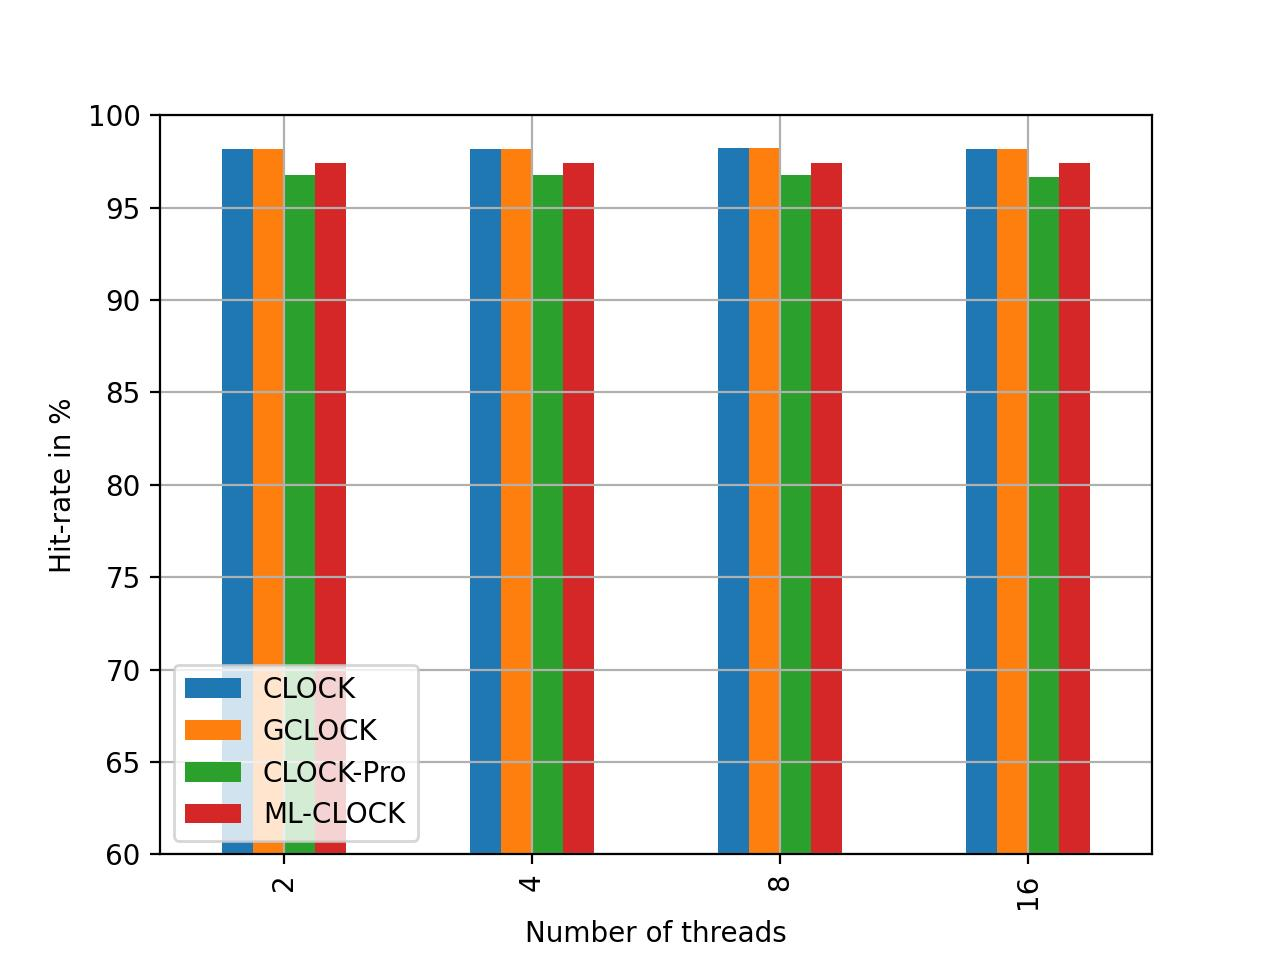
\includegraphics[width=\textwidth]{multi_128_gb_randread_normal.jpg}		
		\caption{128 GiB file size}
		\label{fig:rw_90to10  uniform}
	\end{subfigure}
	\caption{These figures show the hit-rate for each implemented cache replacement policy for normal-distribution random read only workload.}
\end{figure}

\begin{figure}[H]
	\centering
	\begin{subfigure}{0.4\textwidth}
		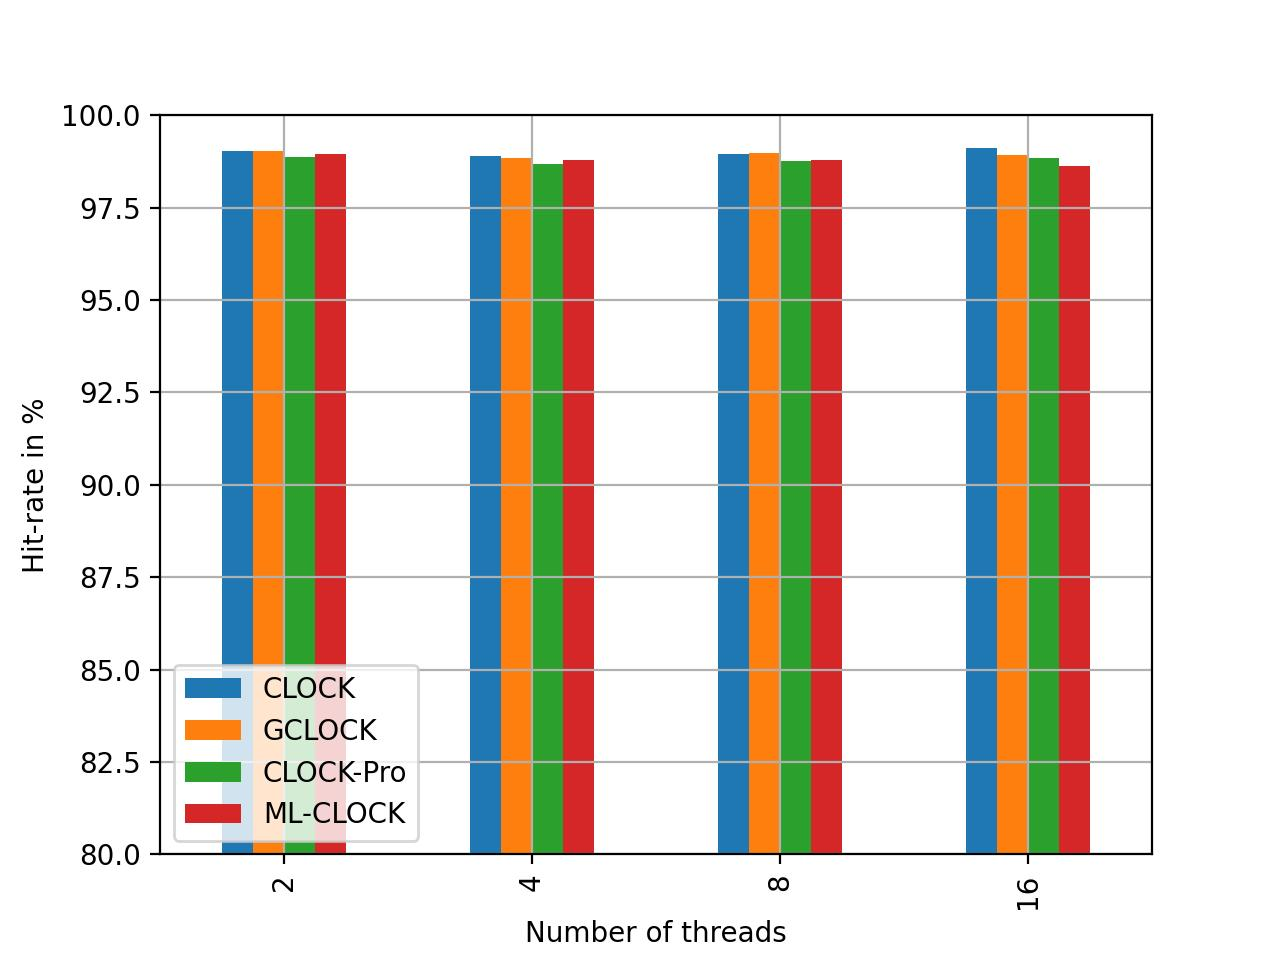
\includegraphics[width=\textwidth]{multi_16_gb_rw_90to10_normal.jpg}		
		\caption{16 GiB file size}
		\label{fig:rw_90to10  zipf}
	\end{subfigure}
	\hfill
	\begin{subfigure}{0.4\textwidth}
		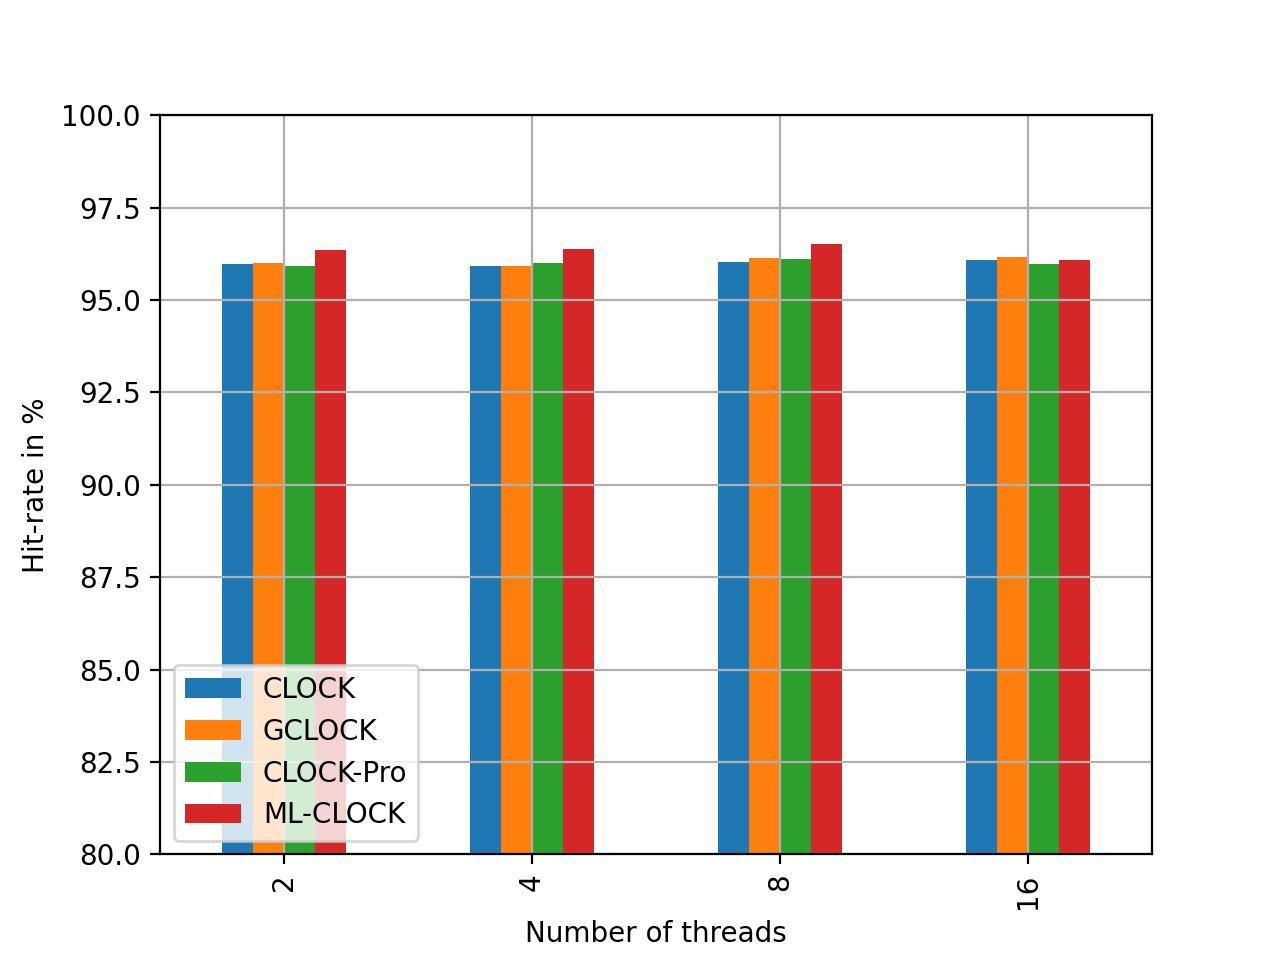
\includegraphics[width=\textwidth]{multi_32_gb_rw_90to10_normal.jpg}		
		\caption{32 GiB file size}
		\label{fig:rw_90to10  normal}
	\end{subfigure}
	\hfill
	\begin{subfigure}{0.4\textwidth}
		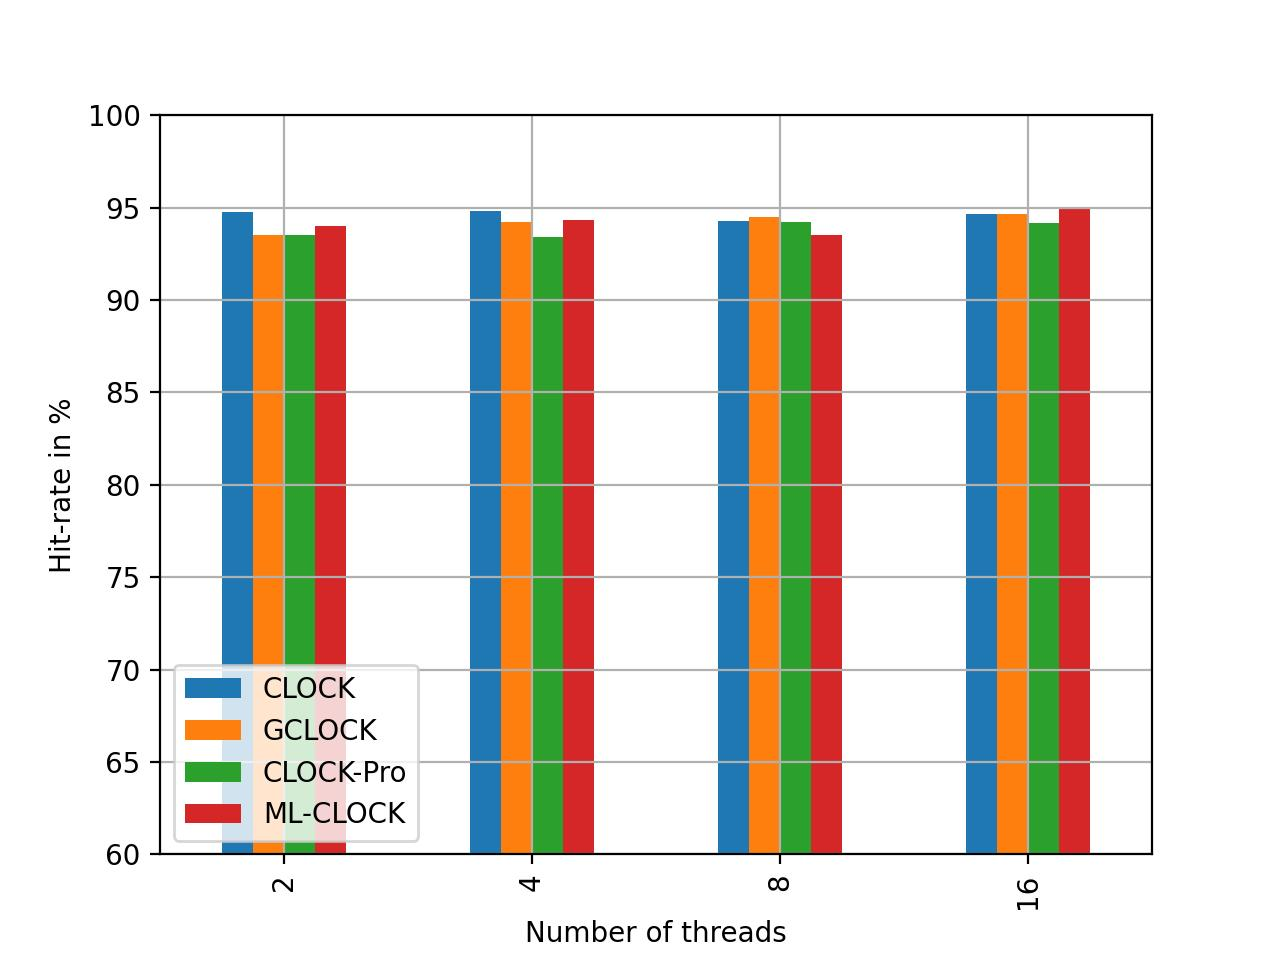
\includegraphics[width=\textwidth]{multi_64_gb_rw_90to10_normal.jpg}		
		\caption{64 GiB file size}
		\label{fig:rw_90to10  zoned}
	\end{subfigure}
	\hfill
	\begin{subfigure}{0.4\textwidth}
		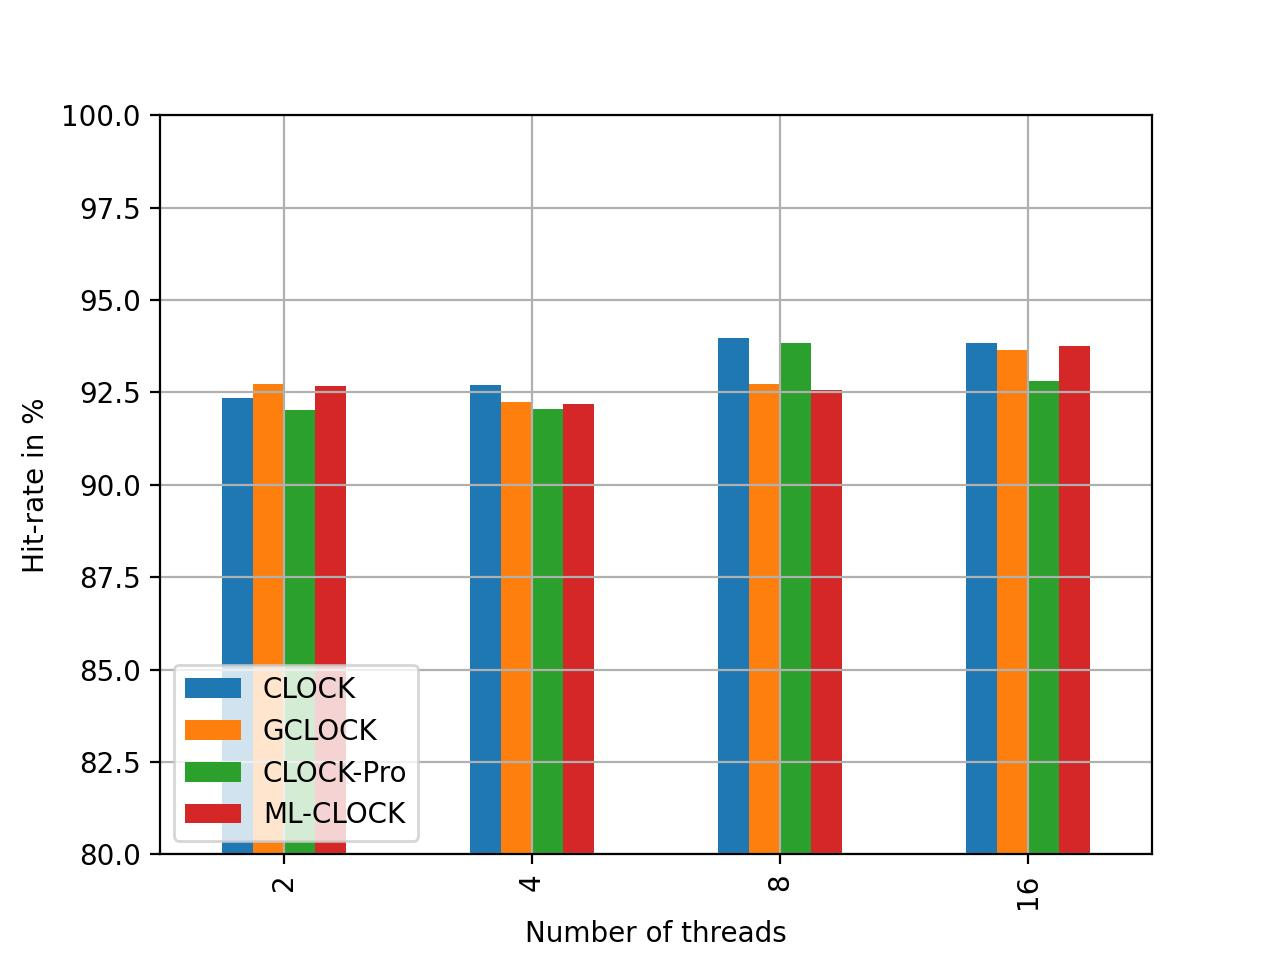
\includegraphics[width=\textwidth]{multi_128_gb_rw_90to10_normal.jpg}		
		\caption{128 GiB file size}
		\label{fig:rw_90to10  uniform}
	\end{subfigure}
	\caption{These figures show the hit-rate for each implemented cache replacement policy for normal-distribution random 90\% read 10\% write workload.}
\end{figure}

\begin{figure}[H]
	\centering
	\begin{subfigure}{0.4\textwidth}
		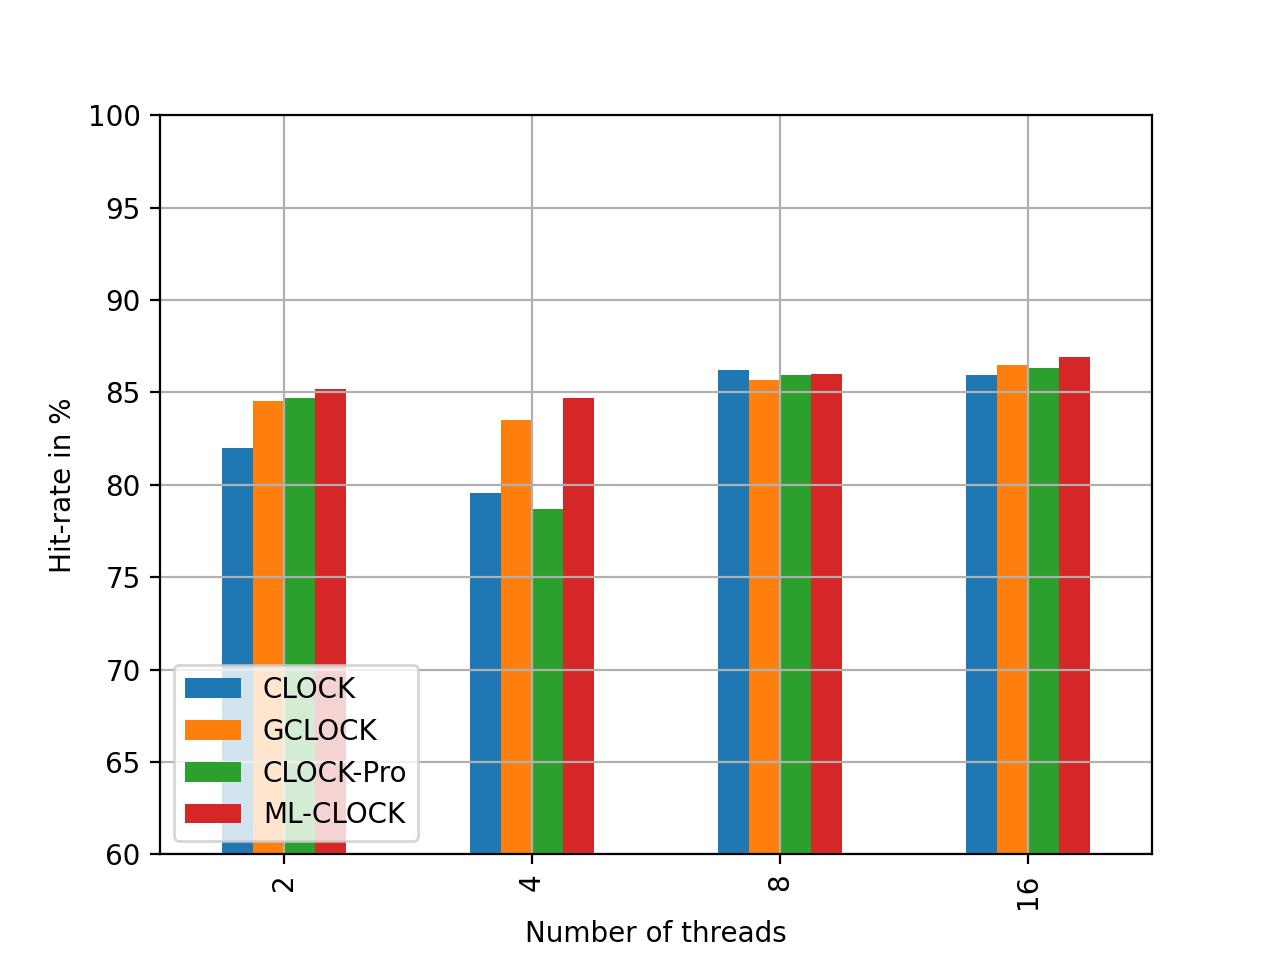
\includegraphics[width=\textwidth]{multi_16_gb_rw_50to50_normal.jpg}		
		\caption{16 GiB file size}
		\label{fig:rw_90to10  zipf}
	\end{subfigure}
	\hfill
	\begin{subfigure}{0.4\textwidth}
		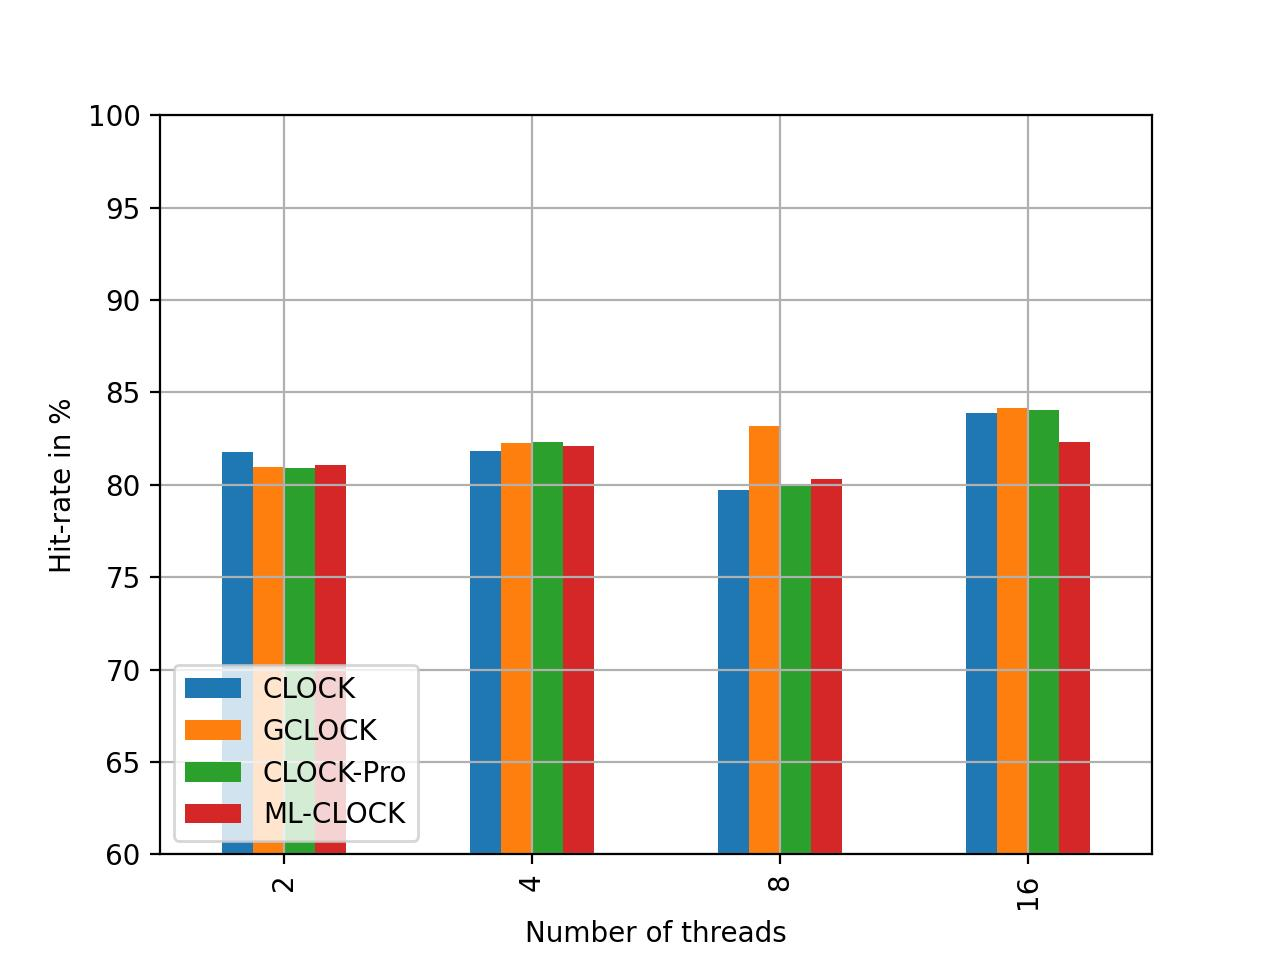
\includegraphics[width=\textwidth]{multi_32_gb_rw_50to50_normal.jpg}		
		\caption{32 GiB file size}
		\label{fig:rw_90to10  normal}
	\end{subfigure}
	\hfill
	\begin{subfigure}{0.4\textwidth}
		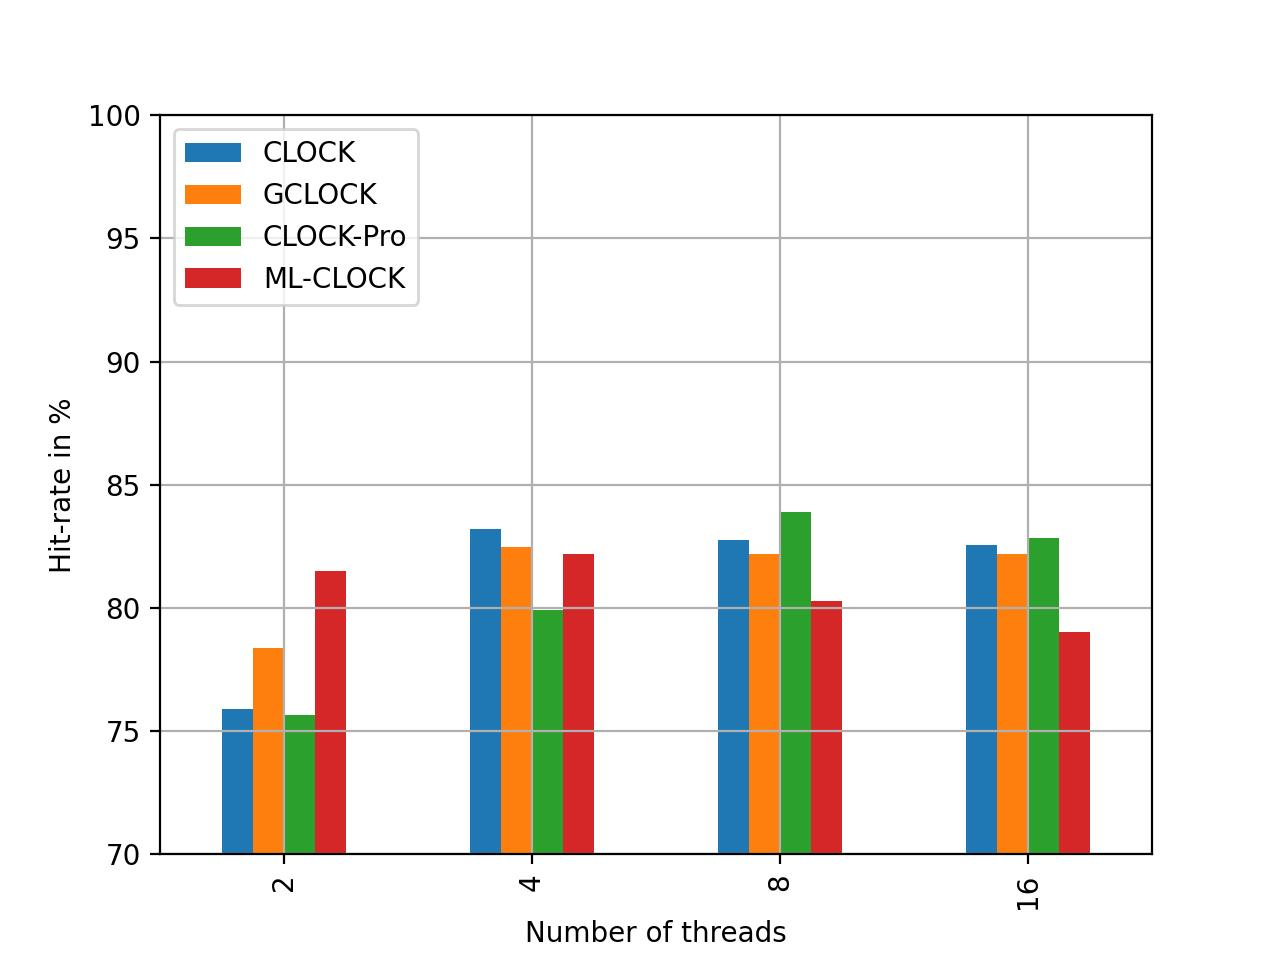
\includegraphics[width=\textwidth]{multi_64_gb_rw_50to50_normal.jpg}		
		\caption{64 GiB file size}
		\label{fig:rw_90to10  zoned}
	\end{subfigure}
	\hfill
	\begin{subfigure}{0.4\textwidth}
		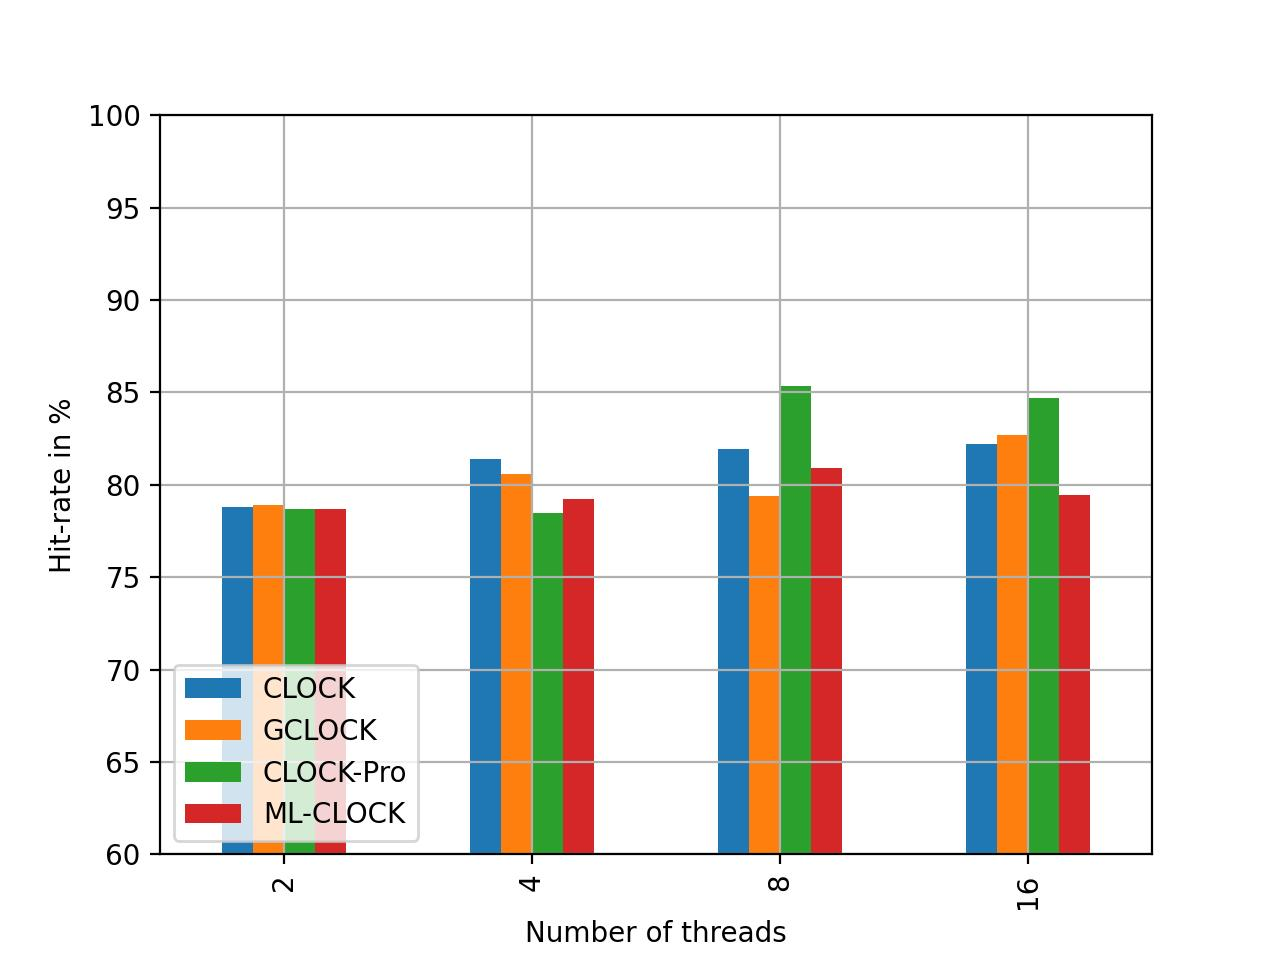
\includegraphics[width=\textwidth]{multi_128_gb_rw_50to50_normal.jpg}		
		\caption{128 GiB file size}
		\label{fig:rw_90to10  uniform}
	\end{subfigure}
	\caption{These figures show the hit-rate for each implemented cache replacement policy for normal-distribution random 50\% read 50\% write workload.}
\end{figure}


%----------------------------------------------

\subsection{Zoned-Distribution Workloads}
\begin{figure}[H]
	\centering
	\begin{subfigure}{0.4\textwidth}
		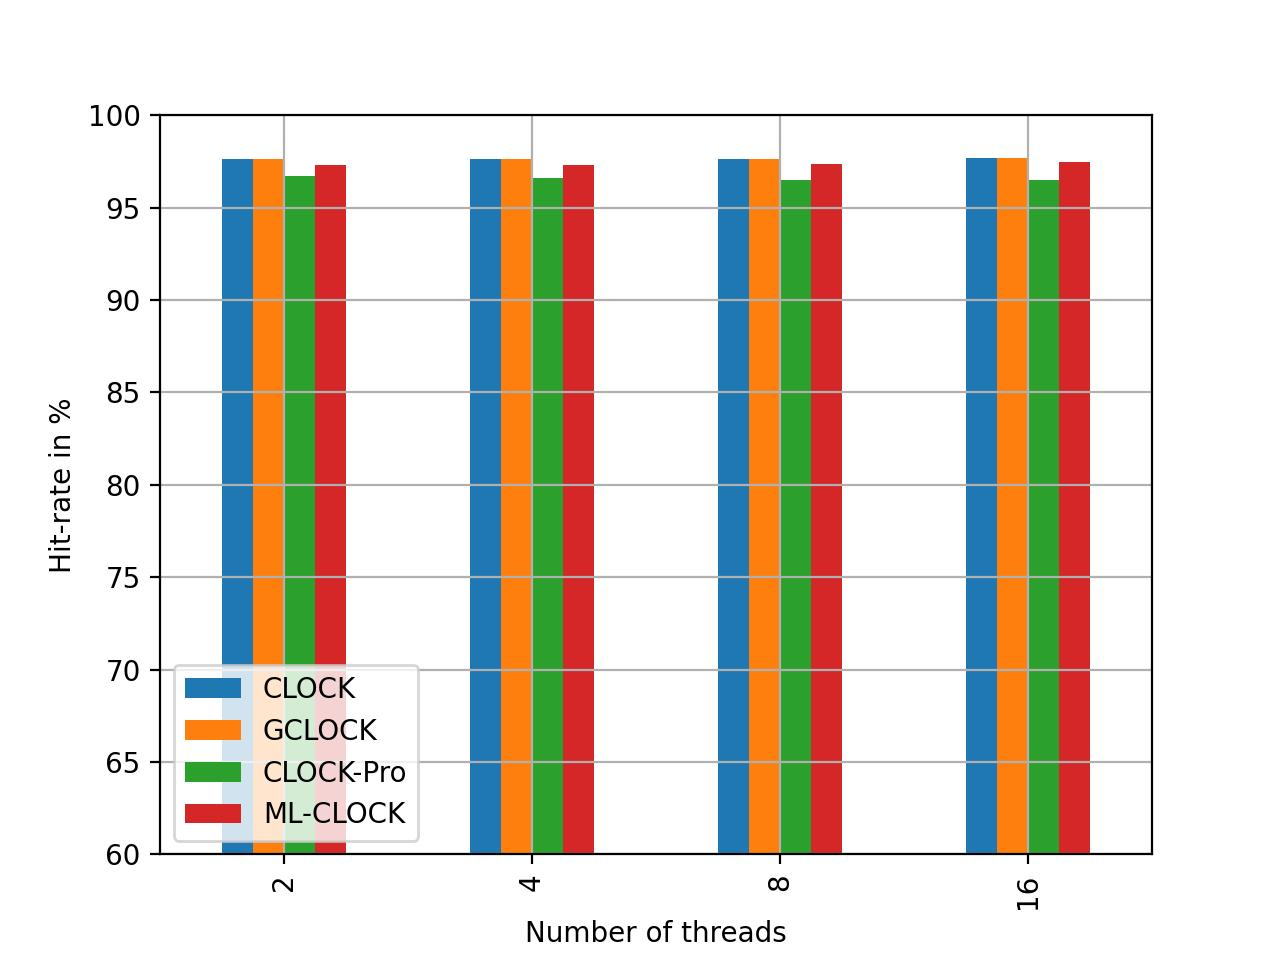
\includegraphics[width=\textwidth]{multi_16_gb_randread_zoned.jpg}		
		\caption{16 GiB file size}
		\label{fig:rw_90to10  zipf}
	\end{subfigure}
	\hfill
	\begin{subfigure}{0.4\textwidth}
		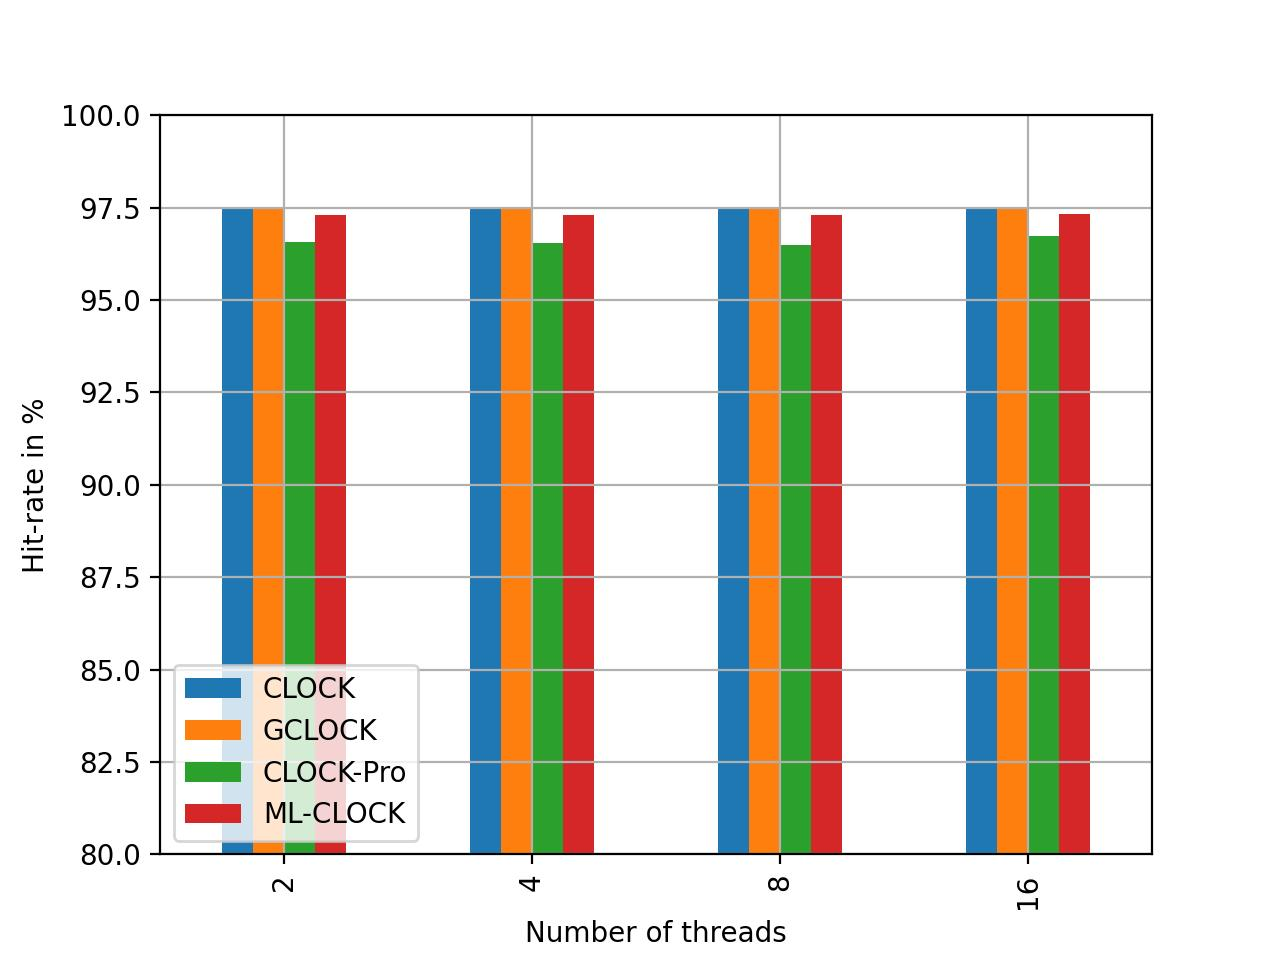
\includegraphics[width=\textwidth]{multi_32_gb_randread_zoned.jpg}		
		\caption{32 GiB file size}
		\label{fig:rw_90to10  normal}
	\end{subfigure}
	\hfill
	\begin{subfigure}{0.4\textwidth}
		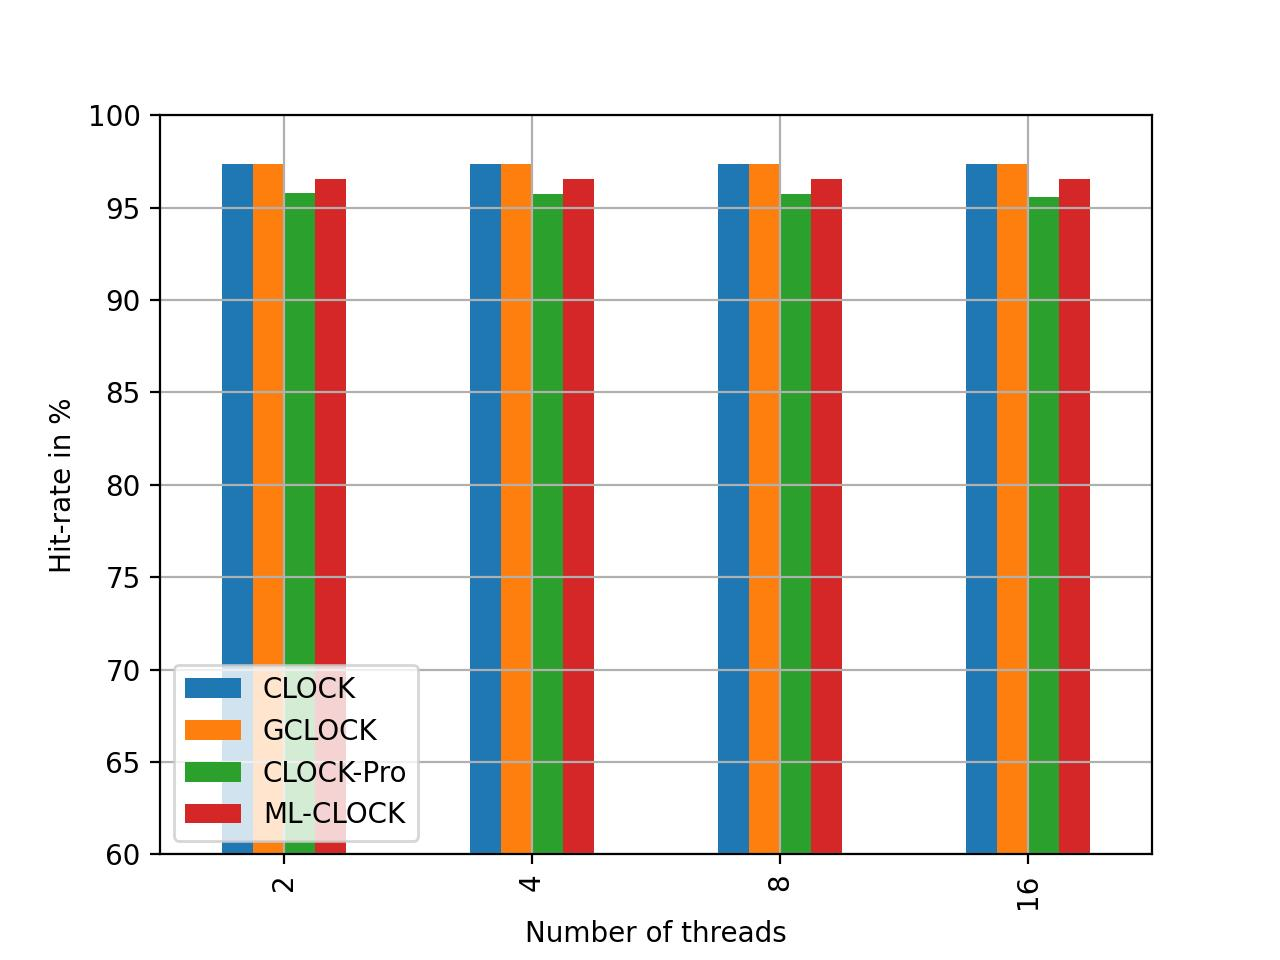
\includegraphics[width=\textwidth]{multi_64_gb_randread_zoned.jpg}		
		\caption{64 GiB file size}
		\label{fig:rw_90to10  zoned}
	\end{subfigure}
	\hfill
	\begin{subfigure}{0.4\textwidth}
		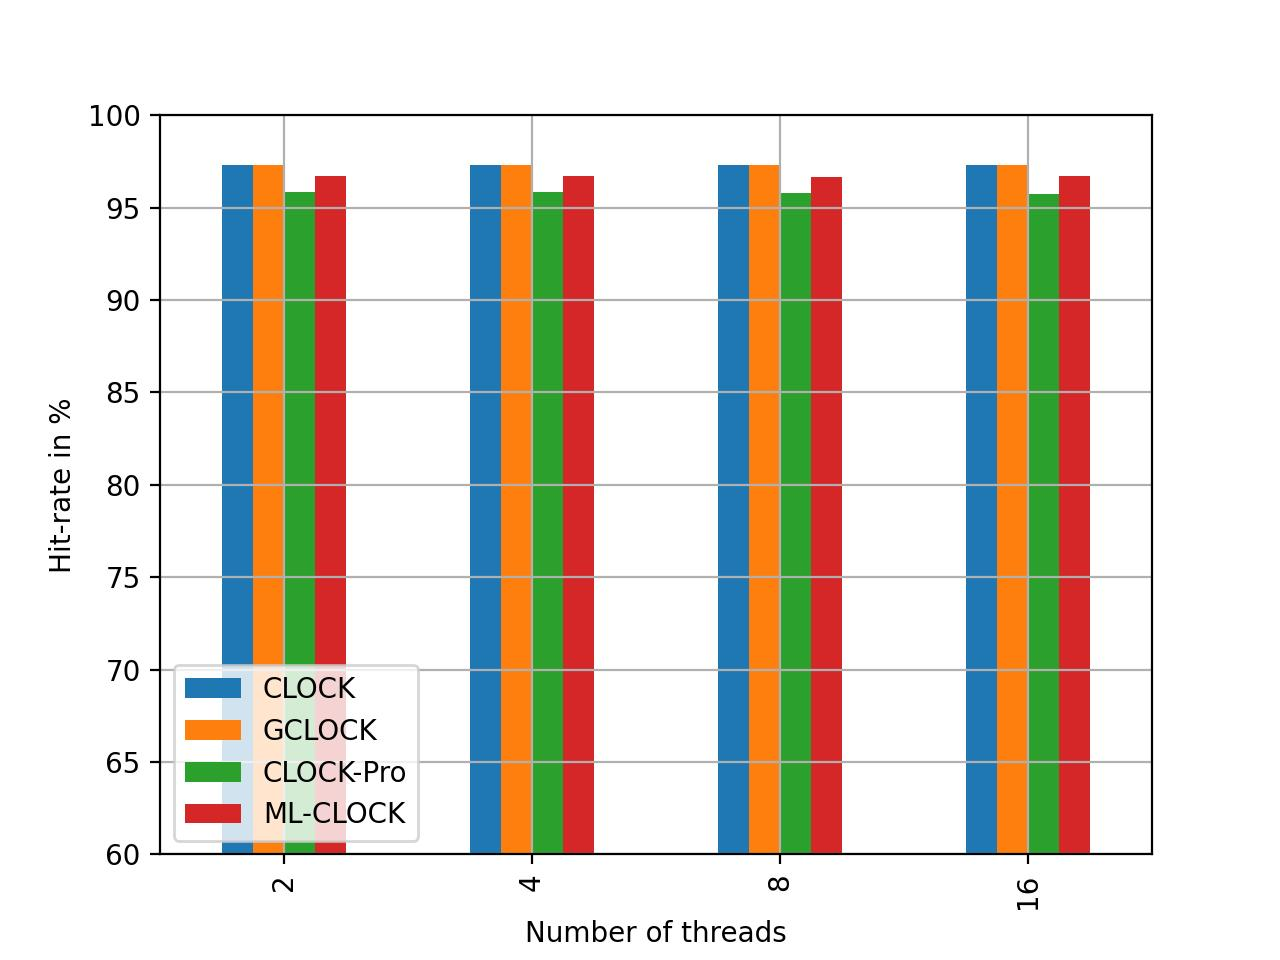
\includegraphics[width=\textwidth]{multi_128_gb_randread_zoned.jpg}		
		\caption{128 GiB file size}
		\label{fig:rw_90to10  uniform}
	\end{subfigure}
	\caption{These figures show the hit-rate for each implemented cache replacement policy for zoned-distribution random read only workload.}
\end{figure}

\begin{figure}[H]
	\centering
	\begin{subfigure}{0.4\textwidth}
		\includegraphics[width=\textwidth]{multi_16_gb_rw_90to10_zoned.jpg}		
		\caption{16 GiB file size}
		\label{fig:rw_90to10  zipf}
	\end{subfigure}
	\hfill
	\begin{subfigure}{0.4\textwidth}
		\includegraphics[width=\textwidth]{multi_32_gb_rw_90to10_zoned.jpg}		
		\caption{32 GiB file size}
		\label{fig:rw_90to10  normal}
	\end{subfigure}
	\hfill
	\begin{subfigure}{0.4\textwidth}
		\includegraphics[width=\textwidth]{multi_64_gb_rw_90to10_zoned.jpg}		
		\caption{64 GiB file size}
		\label{fig:rw_90to10  zoned}
	\end{subfigure}
	\hfill
	\begin{subfigure}{0.4\textwidth}
		\includegraphics[width=\textwidth]{multi_128_gb_rw_90to10_zoned.jpg}		
		\caption{128 GiB file size}
		\label{fig:rw_90to10  uniform}
	\end{subfigure}
	\caption{These figures show the hit-rate for each implemented cache replacement policy for zoned-distribution random 90\% read 10\% write workload.}
\end{figure}

\begin{figure}[H]
	\centering
	\begin{subfigure}{0.4\textwidth}
		\includegraphics[width=\textwidth]{multi_16_gb_rw_50to50_zoned.jpg}		
		\caption{16 GiB file size}
		\label{fig:rw_90to10  zipf}
	\end{subfigure}
	\hfill
	\begin{subfigure}{0.4\textwidth}
		\includegraphics[width=\textwidth]{multi_32_gb_rw_50to50_zoned.jpg}		
		\caption{32 GiB file size}
		\label{fig:rw_90to10  normal}
	\end{subfigure}
	\hfill
	\begin{subfigure}{0.4\textwidth}
		\includegraphics[width=\textwidth]{multi_64_gb_rw_50to50_zoned.jpg}		
		\caption{64 GiB file size}
		\label{fig:rw_90to10  zoned}
	\end{subfigure}
	\hfill
	\begin{subfigure}{0.4\textwidth}
		\includegraphics[width=\textwidth]{multi_128_gb_rw_50to50_zoned.jpg}		
		\caption{128 GiB file size}
		\label{fig:rw_90to10  uniform}
	\end{subfigure}
	\caption{These figures show the hit-rate for each implemented cache replacement policy for zoned-distribution random 50\% read 50\% write workload.}
\end{figure}

%----------------------------------------------

\subsection{Uniform-Distribution Workloads}
\begin{figure}[H]
	\centering
	\begin{subfigure}{0.4\textwidth}
		\includegraphics[width=\textwidth]{multi_16_gb_randread_uniform.jpg}		
		\caption{16 GiB file size}
		\label{fig:rw_90to10  zipf}
	\end{subfigure}
	\hfill
	\begin{subfigure}{0.4\textwidth}
		\includegraphics[width=\textwidth]{multi_32_gb_randread_uniform.jpg}		
		\caption{32 GiB file size}
		\label{fig:rw_90to10  normal}
	\end{subfigure}
	\hfill
	\begin{subfigure}{0.4\textwidth}
		\includegraphics[width=\textwidth]{multi_64_gb_randread_uniform.jpg}		
		\caption{64 GiB file size}
		\label{fig:rw_90to10  zoned}
	\end{subfigure}
	\hfill
	\begin{subfigure}{0.4\textwidth}
		\includegraphics[width=\textwidth]{multi_128_gb_randread_uniform.jpg}		
		\caption{128 GiB file size}
		\label{fig:rw_90to10  uniform}
	\end{subfigure}
	\caption{These figures show the hit-rate for each implemented cache replacement policy for uniform-distribution random read only workload.}
\end{figure}

\begin{figure}[H]
	\centering
	\begin{subfigure}{0.4\textwidth}
		\includegraphics[width=\textwidth]{multi_16_gb_rw_90to10_uniform.jpg}		
		\caption{16 GiB file size}
		\label{fig:rw_90to10  zipf}
	\end{subfigure}
	\hfill
	\begin{subfigure}{0.4\textwidth}
		\includegraphics[width=\textwidth]{multi_32_gb_rw_90to10_uniform.jpg}		
		\caption{32 GiB file size}
		\label{fig:rw_90to10  normal}
	\end{subfigure}
	\hfill
	\begin{subfigure}{0.4\textwidth}
		\includegraphics[width=\textwidth]{multi_64_gb_rw_90to10_uniform.jpg}		
		\caption{64 GiB file size}
		\label{fig:rw_90to10  zoned}
	\end{subfigure}
	\hfill
	\begin{subfigure}{0.4\textwidth}
		\includegraphics[width=\textwidth]{multi_128_gb_rw_90to10_uniform.jpg}		
		\caption{128 GiB file size}
		\label{fig:rw_90to10  uniform}
	\end{subfigure}
	\caption{These figures show the hit-rate for each implemented cache replacement policy for uniform-distribution random 90\% read 10\% write workload.}
\end{figure}

\begin{figure}[H]
	\centering
	\begin{subfigure}{0.4\textwidth}
		\includegraphics[width=\textwidth]{multi_16_gb_rw_50to50_uniform.jpg}		
		\caption{16 GiB file size}
		\label{fig:rw_90to10  zipf}
	\end{subfigure}
	\hfill
	\begin{subfigure}{0.4\textwidth}
		\includegraphics[width=\textwidth]{multi_32_gb_rw_50to50_uniform.jpg}		
		\caption{32 GiB file size}
		\label{fig:rw_90to10  normal}
	\end{subfigure}
	\hfill
	\begin{subfigure}{0.4\textwidth}
		\includegraphics[width=\textwidth]{multi_64_gb_rw_50to50_uniform.jpg}		
		\caption{64 GiB file size}
		\label{fig:rw_90to10  zoned}
	\end{subfigure}
	\hfill
	\begin{subfigure}{0.4\textwidth}
		\includegraphics[width=\textwidth]{multi_128_gb_rw_50to50_uniform.jpg}		
		\caption{128 GiB file size}
		\label{fig:rw_90to10  uniform}
	\end{subfigure}
	\caption{These figures show the hit-rate for each implemented cache replacement policy for uniform-distribution random 50\% read 50\% write workload.}
\end{figure}

\section{Summary}

-> coming soon

\chapter{Conclusion}
\label{cha:conclusion}
% could be conclusions and future work

\section{Future Work}

-> after evaluation

% 5-10%, 2-5 Seiten


\bibliographystyle{apalike}
\bibliography{thesis}

% \backmatter
% should be around 20 references for bachelor thesis
% avoid to cite web sites


\appendix

%\chapter{Appendix}
%\label{cha:appendix}

% could also be ad the beginning
% implement acronyms or list of Abbreviations

%\setcounter{tocdepth}{1}
%\listoffigures
%\setcounter{tocdepth}{1}
%\listoftables
%\lstlistoflistings

\chapter*{}

\section*{Statement of Authorship}

I herewith assure that I wrote the present thesis independently, that the thesis has not been partially or fully submitted as graded academic work and that I have used no other means than the ones indicated.
I have indicated all parts of the work in which sources are used according to their wording or to their meaning.

I am aware of the fact that violations of copyright can lead to injunctive relief and claims for damages of the author as well as a penalty by the law enforcement agency.

\bigskip

Magdeburg, \today

\bigskip
\bigskip

\rule{0.5\textwidth}{0.5pt}\\
\hspace*{0.25em}Signature

\end{document}

%-> can start with this chapter when I decide which benchmark and metrics I want to use\\
%- fio for synthetic benchmarks -> zipf dis. and sequential should be covered\\
%- try to find traces which I can use easily \\
%- some articles uses SPEC-Benchmark traces\\
%
%- general problem that we are dealing with variable sized cache entries and also \\
%  pinning an entry is possible which increases the difficulty of implementation of most suggested algorithms\\
%- most algorithms based an equally sized pages/entries without pinning\\
%- ml-clock with extra locking which could lead to problems, clock and clock-pro uses atomics to prevent this

